% Choose the language of your thesis passing 'french' or 'english' as
% \documentclass option.
% Note1: The 'page de garde' will always be written in French.
% Note2: You will have an error if you change the language of the document and
%        compile it without cleaning the auxiliary files. Compiling it again
%        should solve the problem.
\documentclass[english,a4paper,11pt,twoside]{StyleThese}
\newcommand{\included}{}

\include{formatAndDefs}
\usepackage[colorinlistoftodos,prependcaption,textsize=tiny]{todonotes}
\usepackage{xargs}   % Use more than one optional parameter in a new commands
\usepackage{xcolor}  % Coloured text

\usepackage{amsmath}
\usepackage{amssymb}
\usepackage{mathbbol}

\usepackage{booktabs}

\usepackage{listings}
\usepackage[normalem]{ulem}
\useunder{\uline}{\ul}{}

\newtheorem{theorem}{Theorem}

\usepackage{algorithm}
\usepackage[noend]{algpseudocode} 
% limit indentation in algorithms
\algrenewcommand\algorithmicindent{1.0em}%
\algnewcommand{\IIf}[1]{\State\algorithmicif\ #1\ \algorithmicthen}
\algnewcommand{\EndIIf}{\unskip\ \algorithmicend\ \algorithmicif}

%%%%%%%%%%%%%%%%%%%%%%%%
%	  TODO commands    %
%%%%%%%%%%%%%%%%%%%%%%%%

\newcommandx{\unsure}[2][1=]{\todo[linecolor=red,backgroundcolor=red!25,bordercolor=red,#1]{#2}}
\newcommandx{\change}[2][1=]{\todo[linecolor=blue,backgroundcolor=blue!25,bordercolor=blue,#1]{#2}}
\newcommandx{\info}[2][1=]{\todo[linecolor=olive,backgroundcolor=olive!25,bordercolor=olive,#1]{#2}}
\newcommandx{\improvement}[2][1=]{\todo[linecolor=violet,backgroundcolor=violet!25,bordercolor=violet,#1]{#2}}
\newcommandx{\thiswillnotshow}[2][1=]{\todo[disable,#1]{#2}}

%%%%%%%%%%%%%%%%%%%%%%%%
%	Knowledge bases    %
%%%%%%%%%%%%%%%%%%%%%%%%

\newcommand \kb{K}

% Ontology definition

\newcommand \kbs{\kb_S}
\newcommand \Abox{\mathbb{A}}
\newcommand \Tbox{\mathbb{T}}
\newcommand \Rbox{\mathbb{R}}

\newcommand \propset{P}
\newcommand \classset{T}
\newcommand \indivset{A}
\newcommand \relationset{R}
\newcommand \annotationset{E}

\newcommand \domainset{Dom}
\newcommand \rangeset{Ran}
\newcommand \inclset{Incl}
\newcommand \invset{Inv}
\newcommand \inheritset{C}

\newcommand \indiv{a}
\newcommand \class{t}

\newcommand \labelfunc {\mathcal{L}}
\newcommand \alabel{\mathcal{L}_a}
\newcommand \tlabel{\mathcal{L}_t}
\newcommand \plabel{\mathcal{L}_p}
\newcommand \alabelag[1]{\mathcal{L}_{a#1}}
\newcommand \tlabelag[1]{\mathcal{L}_{t#1}}
\newcommand \plabelag[1]{\mathcal{L}_{p#1}}

\newcommand \subject{s}
\newcommand \property{p}
\newcommand \object{o}
\newcommand \relation{r}

\newcommand{\sparql}{\textsc{sparql}}

% Timeline definition

\newcommand \kbe{\kb_E}
\newcommand \tinterval{\mathcal{T}}
\newcommand \tstart{\tau_s}
\newcommand \tend{\tau_e}

%%%%%%%%%%%%%%%%%%%%%%%%
%	      REG          %
%%%%%%%%%%%%%%%%%%%%%%%%

\newcommand \goalindiv{\indiv_t}
\newcommand \usablepropset{U}
\newcommand \problem{\mathcal{P}}
\newcommand \solution{\mathcal{S}}

\newcommand \costfunc{\mathcal{C}}
\newcommand \varset{X}
\newcommand \var{x}

\newcommand \cost{\mathbb{c}}
\newcommand \node{\mathbb{n}}
\newcommand \state{\mathbb{s}}
\newcommand \action{\mathbb{a}}

\newcommand \softdiff{\,\delta\,}
\newcommand \harddiff{\,\Delta\,}

\usepackage[acronym]{glossaries}

\makenoidxglossaries

\newacronym{hri}{HRI}{Human Robot Interaction}

\newacronym{hatp}{HATP}{Hierarchical Agent-based Task Planner}
\newacronym{htn}{HTN}{Hierarchical Task Network}
\newacronym{het}{HET}{Hierarchical Execution Trace}

\newacronym{reg}{REG}{Referring Expression Generation}
\newacronym{re}{RE}{Referring Expression}
\newacronym{kb}{KB}{Knowledge Base}
\newacronym{mummer}{MuMMER}{MultiModal Mall Entertainment Robot}

\newacronym{ce}{CE}{Compound Entity}
\newacronym{cr}{CR}{Compound Relation}
\newacronym{ct}{CT}{Compound Tree}

\newacronym{ucs}{UCS}{Uniform-Cost Seach}
\newacronym{ia}{IA}{Incremental Algorithm}
\newacronym{gba}{GBA}{Graph-Based Algorithm}

\newacronym{ssr}{SSR}{Semantic Spatial Representation}



%% This is file `example.tex',
%% Copyright 2013 Tristan GREGOIRE
%% Copyright 2015 Yann BACHY
%
% This work may be distributed and/or modified under the
% conditions of the LaTeX Project Public License, either version 1.3
% of this license or (at your option) any later version.
% The latest version of this license is in
%   http://www.latex-project.org/lppl.txt
% and version 1.3 or later is part of all distributions of LaTeX
% version 2005/12/01 or later.
%
%
% This work has the LPPL maintenance status `maintained'.
% 
% The Current Maintainer of this work is T. GREGOIRE
%

%\documentclass{book}

% Loading the tlsflyleaf.sty package require some option to define the
% establishment name, the doctoral school and the PhD speciality.
% In that aim you have 2 key-value option:
%   - Ets=<value> : define the establishment name
%   - ED=<value>  : define the doctoral school and speciality
%   - ED2=<value> : define the second speciality ("double mention"). OPTIONAL.
% The full list of accepted values for each option could be find either
% in the documentation or in ED-list.txt and Ets-list.txt files provide with the package.
%\usepackage[ED=MITT - STICRT, Ets=INSA]{tlsflyleaf}
%\usepackage[ED=SDU2E-Ast, ED2=SDU2E-Eco, Ets=UT3]{tlsflyleaf}
%\usepackage[ED=MITT - STICRT, Ets=UT3]{tlsflyleaf}

% ==================
% Setup basic string
% - PhD Title
% - author
% - defence date
% - laboratory
% - cotutelle
\title{\textbf{\large Knowledge representation and exploitation for interactive and cognitive robots}}
\author{Guillaume SARTHOU}
\defencedate{Date de défense (20/09/2021)}
\lab{LAAS-CNRS}
%\cotutelle{}

% ==================
% Setup people like your boss, the jury team and the referees
% - First you need to define how number they will be in each category
%   It is done with the commands \nboss{n}, \nreferee{n} and \njudge{n}.
%   You can define more people in each category than the number given 
%   but only the first "\npeople" will be print.
% - Then use the command \makesomeone{<category>}{<number>}{<name>}{<status>}{<other>}
%   where:
%     <category> should be select in ['boss', 'referee', 'judge']
%     <number>   is the rank for printing the person. 
%                Only number <= "\npeople" will be printed
%     <name>     First name and las name of the people
%     <status>   Is (s)he a "charg\'e de recher" ou un "professeur d'universit\'e"...
%     <other>    What ever string you want to add (laboratory, jury member place...).
%% Boss
\nboss{2}
\makesomeone{boss}{2}{Aur\'elie CLODIC}{}{}  % Sera affiche en second
\makesomeone{boss}{1}{Rachid ALAMI}{}{} % Sera afiche en premier
%% Referee
\nreferee{2}
\makesomeone{referee}{1}{Michael BEETZ}{}{}
\makesomeone{referee}{2}{Paulo MENEZES}{}{}
%% Jury
\njudge{6}
\makesomeone{judge}{1}{Michael BEETZ}{Professeur}{Rapporteur}
\makesomeone{judge}{2}{Paulo MENEZES}{Professeur Associ\'e}{Rapporteur}
\makesomeone{judge}{3}{Rachid ALAMI}{Directeur de Recherche}{Directeur de Thèse}
\makesomeone{judge}{4}{Aur\'elie CLODIC}{Ing\'enieure de Recherche}{Directrice de Thèse}
\makesomeone{judge}{5}{Simon LACROIX}{Directeur de Recherche}{Membre du Jury}
\makesomeone{judge}{6}{Kerstin FISCHER}{Professeure Associ\'ee}{Membre du Jury}

% ============================================================
% DOCUMENT
%\begin{document}
%   \makeflyleaf
%\end{document}


\sloppy
\begin{document}

\makeflyleaf

\cleardoublepage

\dominitoc

\pagenumbering{roman}

 \cleardoublepage

% Here you can see an example of how to create text conditioned by the language
% variable. The \iftoggle command:
%
%   \iftoggle{ThesisInEnglish}{%
%   <your-text-in-english>
%   }{%
%   <your-text-in-french>
%   }
%
% will compile only one of the two blocks, depending on the variable you set at
% the beginning of this document. Language selection is managed this way in the
% formatAndDefs.tex file. You too can create sections of your thesis that is
% language dependend this way, although you probably won't need it. Another use
% of \iftoggle can be found at the end of this file.
\iftoggle{ThesisInEnglish}{%
\section*{Acknowledgments}
}{%
\section*{Remerciements}
}

A faire en dernier :-) 

\tableofcontents

%\printnomenclature
\printnoidxglossary[type=\acronymtype]
% Use \mtcfixnomenclature below if you have a glossary (added with
% \printnomenclature above) and you're see a shift in the mini-table of
% contents at the begining of each chapter (example: no mini-toc in chapter 1;
% mini-toc of chapter 1 appearing in chapter 2; and so on).
%
% You should not use \mtcfixnomenclature if you have no glossary (that means,
% if you don't use \printnomenclature or if your glossary is empty).
%\mtcfixnomenclature

\mainmatter


\ifdefined\included
\else
\setcounter{chapter}{0} %% Numéro du chapitre précédent ;)
\dominitoc
\faketableofcontents
\fi

\chapter{Introduction}
\minitoc

To introduce this thesis and provide a global picture of its content, we first narrate a short story about a robot in a store. This story will then be used to identify some of the mains abilities a robot need to interact with humans with a focus on the knowledge it needs. While this thesis is from a roboticist point of view, working on interaction naturally leads to the study of cognitive psychology. From this field, we want to present an overview of the knowledge organisation models that have had an impact on the field, at the point to be now used for robotic researches.

\section{A prototypical scenario}

A company selling cameras have recently invested in a robot to support its employees in its stores. Their goal with these robots is to helps the employees during their daily tasks in the stores. The robots can prepare commands, put items on the shelves, cash customers, or advise them.

Max is one of these robots. It is a Pr2 design equipped with a head, two arms, and a mobile base with wheels. It is 9 a.m. and the robotic company having produce Max, power it on for the first time in the store. The robot starts navigating in the store, looking at all the products on the shelves. Liam, the human employee is counting the cash register when a customer enters the store. This customer is Tony. He looks to some cameras exposed on the shelves, going from one shelf to another.

Max, seeing Tony looking at all the cameras and Liam occupied to count the cash register, decides to go to see if the customer needs help.

\begin{quote} 
\centering 
\textit{
- "Hi, I am Max. Have you found a camera interesting you or do you need some advice?" \\
- "Hi, I don't really know anything about cameras. I go on a trip in a month and I would like a camera to take animal pictures during the trip." }
\end{quote}

For an amateur, Max chooses to present to Tony some automatic models. Moreover, since it is for a trip, he advises Tony to prefer a small camera. Looking at the prices, the customer explains that he did not want to spend more the 500 euros. Max thus select three options for him:

\begin{quote} 
\centering 
\textit{
- "You have this one at 350, the small black one here in front of you at 475, and on the other shelf there the small brown one near to the screen at 230." }
\end{quote}

\begin{figure}[h!]
\centering
\includegraphics[width=\textwidth]{figures/introduction/camera_store_2.png}
\caption{\label{fig:cam_store} A Pr2 robot, as an employee of a camera store, advises a customer. }
\end{figure}

Explaining that, Max point to the cameras. They continue to discuss when Tony's phone rings. He has to go to join his wife. In another store in the mall. Not knowing where the other store is he said:

\begin{quote} 
\centering 
\textit{
- "I am sorry I have to go. I will come back in the week. I have to go to a store selling video game but I do not remember the name." \\
- "There is only one store selling video games in this mall, it is Game-ania." \\
- "Do you know how to reach it from there ?" \\
- "For sure"}
\end{quote}

Max slowly moves next to the entrance, followed by Tony. It raises one arm pointing to the aisle and said:

\begin{quote} 
\centering 
\textit{
- "Go down this aisle then turn left straight after the salad bar. After that Game-ania will be on your right when we walk."}
\end{quote}

Tony goes and come back the next morning. Max recognizing him, goes towards him. It asks Tony if he easily found the video game shop and recall the camera identified the day before.

\begin{quote} 
\centering 
\textit{
- "Yesterday we stop on two Fujifilm cameras and a Canon for your trip."}
\end{quote}

They continue to discuss and finally Tony selects the camera at 350 euros. Following Max's advice, takes a memory card and a second battery to have enough storage and power during his trip. In addition, he takes a lens to take pictures of animals from far. Unfortunately, the wanted camera is not available at the moment. The last in the store is the demonstration one. Max purpose to Tony to command it. The client agrees and goes.

A few days later, before opening, several boxes arrive at the store. Liam, the human employee, and Max have to open them, fill the stocks and prepare Tony's command. This is the first time since Max arrival they have to do it. They both go to the backroom to do this task together. There are two boxes. Liam starts opening one so Max starts opening the other. Max informs Liam about the camera which should arrive.

\begin{quote} 
\centering 
\textit{
- "Tell me if their is a X-T100, a customer commands one."}
\end{quote}

\begin{figure}[h!]
\centering
\includegraphics[width=\textwidth]{figures/introduction/camera_store_3.png}
\caption{\label{fig:cam_store} A Pr2 robot and a human employee collaborating to close a box. }
\end{figure}

Liam finds the camera. The robot explains to him that it also need an SD card of 32Go and a lens XC 15-45mm. It informs the human that the SD cards are too small for it to grasp them. It thus purposes to Liam to take some of the cameras to put on the shelves and to bring back the card and the lens at the same time. During this time, Max takes a box, put the camera in and the battery. When Liam comes back, he put the two other items in the same box. Then, Max maintains the box close while Liam scotch it. When finished, they both take the last items to put on the shelves and go to the main room.

The afternoon of the same day, Max is cashing in a customer. Tony enter is the store. Seeing him, it request Liam:

\begin{quote} 
\centering 
\textit{
- "Can you bring the command we prepared this morning? The client it is for is the one just entering, with the blue T-shirt."}
\end{quote}

Liam goes into the back room and brings back the correct box. Max cash the customer how finally get his camera in the time.

\section{Interacting with a robot: What can we expect ?}

\section[Knowledge organization]{Knowledge organization: Drawing inspiration from cognitive psychology }

Even if our goal in robotics is not to create a copy of the human, either in terms of body shape or cognition, drawing inspiration from it is nevertheless important. In the same way that roboticists take inspiration from the human body to create robots able to evolve in a world created by and for the human, the field of cognitive robotics takes inspiration of the human cognition to create robots able to interact with humans. While we do not aim to make a copy of human cognition, we think that a robot must endow similar capabilities if we want them to interact with us efficiently and in an acceptable way.

Regarding the knowledge representation, the first experimental study has been realized in 1885 by Ebbinghaus~\cite{ebbinghaus_1885_gedachtnis}. Since then, the definition of memory as the capacity to encode, store, and retrieve knowledge \cite{roediger_1996_retrieval} has been widely accepted. At the same time, the word "memory" has become a generic term suggesting a unique system. However, the human memory can rather be seen as several sub-systems that differ from their storage duration, storage capacity, and the level of consciousness necessary for information retrieval. In the rest of the section, we present some memory models, presented in a non-chronological way, and focussing on what is called long-term memory. During all this section, it is important to keep in mind that we only present models aiming to understand human cognition with a focus on knowledge management. No formal truth is stated here given that there is no consensus in the field. The presented models and terms will allow us to better understand the existing robotic cognitive architectures and give inspiration for the design and structuration of the components developed during this thesis.

\improvement{schema pour chaque model ?}
The primary division of the memory is done concerning the storage duration and capacity. From there has been defined the \textbf{short-term memory} (STM) and the \textbf{long-term memory} (LTM) \cite{atkinson_1966_some}. Short-term memory is characterized by its small capacity and its capability to retrieve information that has just been seen. We often hear about twenty seconds and seven items (or chunks)\improvement{ref}. Long-term memory, on the opposite, refers to any situation where we use information that has not just been seen. We often hear about infinite capacity and duration. It is this latter that allows the acquisition of new knowledge and the retrieval of information acquired a long time ago.

Over the years, what was called short-term memory has become the \textbf{working memory} (WM) \cite{baddeley_1986_dementia}. This change has been made to add a notion of knowledge manipulation. Instead of focusing on the only temporal aspect, it reflects its functional aspect. It is thus a system that retains information for the time necessary for its use by other cognitive functions. The working memory and the long-term memories are two independent but related systems. For information to be stored in long-term memory, we think that it has to pass by the working memory.

For the structure of the long-term memory, a first dichotomy is proposed by Graf and Schacter \cite{graf_1985_implicit} with the \textbf{implicit} and \textbf{explicit} memory. It reflects the way knowledge can be retrieved. Knowledge from explicit memory can be retrieved consciously and voluntarily. On the opposite, knowledge from the implicit memory is retrieved in situations in which our comportments are influenced by an experience. This is the case when you pour water into a glass. We do not need to retrieve explicitly how to perform this task. It is our experience that influences how we do it.

Another dichotomy has been proposed by Squire and Cohen \cite{squire_1982_remote} with the \textbf{procedural} and \textbf{declarative} memory. Procedural memory is the system allowing us to retain knowledge about our cognitive, motor, or perceptual skills. It is the memory of the know-how. A particularity of this memory is that it is difficult to speak about the knowledge it stores and we use them unconsciously. The declarative memory stores representations of facts, events, general knowledge, and memories of past events. This knowledge can be retrieved consciously and we can speak about them. Taking the example of the code of your credit card. Initially, this knowledge is store in the declarative memory. When you need it you can easily remember it at say it. The more you use it and it slowly becomes an automatism. It became hard to remember it consciously while you use it every day and if you need to say it you can type it on a virtual keyboard to remember it. It has slowly moved into your procedural memory. We see that both dichotomies are almost equivalent. The declarative memory of Squire is related to the implicit memory of Graf, and the procedural one is related to the implicit memory.

Going deeper into the declarative memory, Tulving has proposed a dichotomy between \textbf{episodic} and \textbf{semantic} memory \cite{tulving_1995_organization}. The episodic memory retains knowledge related to past experienced events, which are specific to our individual experience, and localized both in space and time. The semantic memory is more general and retains knowledge that we accumulate all along with our life concerning our environment. It can be seen as an encyclopedic memory independent of the acquisition context. While the episodic memory is related to "remembering", the sematic one is related to "knowing". Taking as an example your visit to Toulouse \footnote{If you never visit it, you can take another city you have visited but you should plan to visit it anyway.}, this visit is encoded in the episodic memory while the knowledge that Toulouse is a city in France is encoded in the semantic one.

\begin{figure}[h!]
\centering
\includegraphics[scale=0.45]{figures/introduction/SPI.png}
\caption{\label{fig:SPI} Relations between episodic memory and semantic memory according to the SPI (Serial, Parallel, and Independent) model of Tulving (1995).}
\end{figure}

With the previous example, we saw that even if these two sub-systems of the declarative memory are independent, they are therefore in interaction with eachother as we can apply a semantic treatment on the episodic memory. To better undertand their relation, Tulving has proposed Serial, Parallel, and Independent model (SPI). As illustrated in Figure~\ref{fig:SPI}, the encoding of an information is serial (S) passing first by the semantic memory then in the episodic one. The storage in both memories is performed in parallel (P). Finally, the information recovery is independy between the two memories.
As we explain in the begin of this section, the presented theory can not be proven and must therefore be taken as~\cite{tulving_1995_organization} "an explicit starting point for a more systematic pursuit of what is clearly the next problem that needs to be tackled".

\section{Contributions}

\subsection{Knowledge representation}

\subsection{Knowledge exploitation}

\section{A reader's guide}



\include{Chapter1}
\ifdefined\included
\else
\setcounter{chapter}{2} %% Numéro du chapitre précédent ;)
\dominitoc
\faketableofcontents
\fi

\chapter{Ontologenius: A semantic memory for HRI}
\chaptermark{Ontologenius}
\label{chap:ontologenius}
\minitoc
\label{chap:2}

In this chapter, we present the software Ontologenius. It is a lightweight and open-source software to store an ontology, perform reasoning on it, update it, and query it. Ontologenius has been developed especially for \acrlong{hri} application. In this way, it is able to manage several ontology instances in parallel and puts a focus on the concepts' names in natural language. It aims to be used as a server, shared by an entire robotic architecture, providing consistent and always up to date knowledge to every components of the architecture. Consequently, it is thread-safe and can be queried by several components at a time while being constantly updated.

A previous version of this contribution has been presented and published at the RO-MAN 2019 conference~\cite{sarthou_2019_ontologenius}. Due to the evolution of the software since this publication, the current chapter presents new features and a more mature contribution.

\section{Design and features}

In this section, we first explain our choice to use ontology as a means of representing knowledge, both from the point of view of its expressiveness and its growing use in robotics. Then, we present the wanted features and the level of expressiveness we have selected for this software. Finally, we draw a formalism of the kind of ontology we will use all along this thesis.

\subsection{Why an ontology?}

In cognitive psychology, we saw that semantic memory refers to the encyclopedic knowledge of words associated with their meanings. After several studies about participants response times to questions, some authors have proposed a model of this semantic memory as being a semantic network~\cite{collins_1969_retrieval, collins_1970_does}. With this model, they put the hypothesis that knowledge is organized in a hierarchic way, respecting a principle of inclusion among classes. For example, a class representing the concept of cat would inherit an upper class, representing the concept of animal. In addition, instances of these classes would be linked to others through properties, and in the same way, as for the classes, a notion of hierarchy over the properties would exist. Such a structure of knowledge in humans would allow a cognitive economy as well as efficient storage of this knowledge. Even if they were not the first to formalize the principle of a semantic network, Collins and Quillian have provided prominent works and computer implementations.

As reported in~\cite{prasad_2020_knowledge}, such a semantic network, also called semantic graph or knowledge graph, is today frequently used as knowledge representation in robotic applications to represent among others:

\begin{itemize}
  \item the categories of entities at different levels of abstraction~\cite{balint_2018_variations}, e.g. a handle is a physical object
  \item the characteristics of entities~\cite{tenorth_2017_representations}, e.g. a fridge has a handle
  \item the function or purpose of entities~\cite{paulius_2019_functional}, e.g. the fridge handle allows to open the fridge
  \item the location of an entity regarding another one (i.e. spatial relations)~\cite{singh_2020_fuzzy}, e.g. the milk bottle is in the fridge
\end{itemize}

This is on the basis of this knowledge that we can then create programs to provide cognitive capabilities to robots. Here is an important point, this knowledge should support the components of the architecture but is not necessarily part of it. It is called the knowledge-enabled robot programming paradigm~\cite{beetz_2012_cognition}, where the knowledge is separated from the program. It allows to have several subsystems of a same robotic architecture, each providing a specific cognitive capability but all sharing the same knowledge. The choice to share common knowledge leads to important challenges requiring first to agree on the knowledge content and second to provide it in a machine-understandable way. Considering the use of a semantic network as knowledge representation, the use of ontology has tended to respond to these challenges.

The first definition of an ontology has been proposed by Guber in~\cite{guber_1993_translational} as: \textit{``an ontology is an explicit specification of a conceptualization''}. Later, Borst~\cite{borst_1999_construction}, has introduced two new concepts defining an ontology as a \textit{``formal specification of a shared conceptualization''}. The new concepts are the notions of ``formal'' and ``shared''. Merging these two definitions, Studer et al.~\cite{studer_1998_knowledge} reached the definition: \textit{``An ontology is a formal, explicit specification of a shared conceptualization''}. With this last definition, we start to see that an ontology can be a powerful tool to create a \acrfull{kb} common to an entire robotic architecture and used by subsystems providing specific cognitive capabilities.

Even if all the previous definitions trend to refine what is an ontology, they all rely on the common notion of conceptualization for which no formal definition is provided. A former definition, presented in~\cite{genesereth_1987_logical}, was:

\begin{quote} 
\centering 
\textit{
``A body of formally represented knowledge is based on a conceptualization: the objects, concepts, and other entities that are assumed to exist in some area of interest and the relationships that hold among them. A conceptualization is an abstract, simplified view of the world that we wish to represent for some purpose. Every knowledge base, knowledge-based system, or knowledge-level agent is committed to some conceptualization, explicitly or implicitly.''}
\end{quote}

However, as explained by Guarino in~\cite{guarino_2009_ontology}, such a definition of a conceptualization does not correspond to our intuition either our need for an ontology. Indeed, we do not want the conceptualization to depend on the current situation. It should rather be what is common to any situation, allowing to represent them in a uniform way. As explained in~\cite{guarino_1995_towards}, when the world is modified, the conceptualization should stay the same. We are thus interested in the meaning of the concepts used to describe a world state. However, the final definition of a conceptualization provided by Guarino goes with difficulty in this direction despite its initial goal. For the simplicity of the current purpose, the conceptualization should be the meaning of any concept allowing to represent a given situation or world state. Consequently, an ontology could be defined as:

\begin{quote} 
\centering 
\textit{a formal and explicit specification of the shared meaning of any concept allowing to represent a given situation.}
\end{quote}

In other words, an ontology aims at constraining the interpretation of a used vocabulary. It is thus a logical theory. However, looking at the literature, we notice that the definition of an ontology is still today blurry. Indeed, even if it represents the meaning of the usable concepts, we want to apply it to the \acrshort{kb} representing a given world state, even if it evolves. Where a semantic network would represent this instantiation, because the meaning of its edges could be defined by the use of an ontology, in this thesis, we will use the term ontology to refer to \textbf{a semantic network owning a restriction on the interpretation of the used vocabulary}. As the goal of this thesis is not to model these restriction rules but rather to use them, it should not lead to any confusion.

Considering the study of ontology in robotic, and more generally in computer science, we can distinguish three kinds of contribution:

\begin{itemize}
  \item ontology creation,
  \item ontology storage and inference,
  \item framework using ontology
\end{itemize}

Ontology creation focuses on the definition of vocabulary and rules. The created ontologies are often divided into four categories: upper-level, reference, domain, and application. The upper-level ontologies define widely applicable concepts, transversal to several disciplines. The more used are DOLCE (Descriptive Ontology for Linguistic and Cognitive Engineering) \cite{masolo_2003_dolce}, Cyc \cite{lenat_1989_building}, or SUMO (Suggested Upper Merged Ontology) ~\cite{niles_2001_towards}. Reference ontologies are based on upper-ontology and describe the vocabulary of a discipline, like engineering or medical. For example, \cite{schlenoff_2015_ieee} covers robotics and automation. Domain ontologies aim at refining a discipline, focussing on a more restricted domain in it, like the SOMA ontology~\cite{bessler_2020_foundations} focussing on activities representation. Finally, applications ontologies extend domain ontologies for precise applications. The ontology design uses languages like RDF (Resources Description Framework), FOL (First Order Logic), or OWL (Web Ontology Language). Each language comes with characteristics like formality or computability.

Using these ontologies, numbers of frameworks have been developed to support high-level reasoning process in robotic applications. Among them, we find ontology used for decision making, situation assessment, planning, or belief maintenance. A complete review of these reasoning capabilities and the corresponding frameworks is available in~\cite{olivares_2019_review}. Among the reviewed frameworks, the emblematic ones are KnowRob~\cite{tenorth_2013_knowrob}, ROSETTA~\cite{stenmark_2013_knowledge}, CARESSES~\cite{bruno_2017_caresses}, RoboBrain~\cite{saxena_2014_robobrain}, or ORO~\cite{lemaignan_2010_oro}.

The last contribution type, being the one of the current chapter, is the ontology storage and inference to form a \acrlong{kb} on which the framework can rely to perform high-level reasoning. KnowRob uses Prolog~\cite{wielemaker_2003_prolog} with a library to manage RDF triples. ROSETTA uses a Sesame triple store~\cite{broekstra_2002_sesame}. ORO uses the Jena triple store in addition to the Pellet~\cite{sirin_2007_pellet} reasoner. Finally, RoboBrain uses a custom graph database. We can see that no standard solution has emerged as it mostly depends on the application needs in terms of query capability, expressiveness support, or technical support and compatibility. As other tools we can find in C++ owlcpp~\cite{levin_2011_owl} based on Raptor and Fact++~\cite{tsarkov_2006_fact}, or in Python RDFlib, OWLReady2, or AllegroGraph.

To sum up, a \acrlong{kb} in the form of an ontology, can be viewed as a semantic graph relying on a formal and explicit specification of the shared meaning of concepts used to represent a given situation. In order to be used in a framework to perform high-level reasoning, ontology has to be stored to expose the knowledge it contains to other components. No standard storage solution has emerged so far as it mostly depends on the application needs. Consequently, in the next part of this section, we discuss our needs with a focus on \acrlong{hri} applications and taking inspiration on the existing solutions, we define the features we want for our storage system.

%This initial model has since been formalized as an ontology \cite{berners-lee_semantic_2001} and is already widely used in the semantic web.

\subsection{Desired features}

\paragraph{Work as a server:} The robotic architecture we target is composed of several modules, able to communicate. On the top of the architecture, we consider a supervision system, being a kind of ``puppet-master'' which call each component when needed. A common issue with such an architecture is that each component owns a part of the general knowledge which can lead to inconsistencies. Consequently, the \acrlong{kb} we want should be a server, accessible by query and update by any component. It thus provide uniform knowledge among the architecture. To create a server, we could use any existing tool and attach a communication layer to it. This is for example the case of ORO, which work as a sever, based on the Jena triple store and providing a Telnet interface to send the queries and updates.

\paragraph{Support multiple instances:} Since we target \acrshort{hri} application, we need to be able to represent an estimation of the others knowledge. Where some could use a single \acrlong{kb} to represent the robot knowledge as well as the humans' knowledge, we want our software to support the ``self-other distinction''. It is presented in~\cite{pacherie_2012_phenomenology} as the fact that ``for shared representations (...) to foster coordination rather than create confusion, it is important the agents be able to keep apart representations of their own and other's actions and intentions''. To the best of our knowledge, ORO is the only software proposing this ability. However, it uses a simple way to implement it by running several instances of the same triple store, each attached to an agent. As we will see during this chapter, in robotic application such a solution is not sufficient. For task planning usage, we could need to estimate a future state of a \acrshort{kb}. To implement this feature, we need to be able to capture the state of a \acrshort{kb} at a given instance then be able to modify it without impacting the original \acrshort{kb}. At the date of this thesis, no tool provides this possibility.

\paragraph{Query at the semantic level:} As explained in~\cite{broekstra_2002_sesame}, to query RDF graphs, three levels are possible. Considering an ontology written in XML, the syntactic level would query the XML structure. Consequently, it would query a tree rather than a graph. A query would be ``give me the resources nested in a \textit{Description} element having the attribute \textit{about} with the value X''. It is thus dependant on the language and requires to known the used keywords. The structural level, as available in~\cite{lassila_1998_resource}, provides an abstraction to the language. It allows query of the kind ``give me all the elements of type A'' regardless of how it is represented in the language. However, the structural only looks at the explicit triples. If B is a subtype of A and the element x is described as being of type B, requesting for the elements of type A, x will not be returned. The last query level is the semantic level which is not limited to explicit knowledge. At this level, requesting for the elements of type A, x would be returned as x is of type B and B is a specification of A. This means that we do not consider a simple triple store trying to match patterns. To support this query level, two solutions can be used: computing the closure of the graph (adding A as a type of x and storing it), or inferring it at query. While the first solution removes a part of the semantic by flattening the hierarchy, the second can be time-consuming for the queries.

\paragraph{Specific queries:} We aim to use our software with solver algorithms. This means that we want to provide fine access to the stored knowledge at high frequency. At the difference of Prolog having its own search algorithm, we would prefer lower-level queries such as: ``which are the direct types of X?'', ``which are the inverse properties of Y?'', ``which properties link C and D?'', or ``is E in the domain of application of F?'', and that at the semantic level. Nevertheless, for fast queries, we should be careful with the number of inferences needed at query time.

\paragraph{Reasoning at update:} To avoid too many inferences at query time, we want some inferences to be applied at update. While computing the entire closure would flatten the \acrshort{kb}, some relations can still be computed at updates like the ones coming from inverse relations, or chain axioms.

\paragraph{Thread safe:} Since the software should work as a sever, we want it to support multiple queries in parallel but to be safe on update.

\paragraph{Expressiveness level:} Considering the Web Ontology Language (OWL), it exists different levels of expressiveness depending on the needs. The most expressive one is OWL-full, however, it is said to be not computational, meaning that the inferences it allows cannot be resolved at query time. Then, OWL-DL (Description Logic) supports property and class hierarchy, enumeration value restriction, inverse properties, or cardinality restriction. Finally, OWL-lite is the less expressive one, not supporting the cardinality restriction and the restriction on value. Even if OWL-DL would be suitable, in a first version OWL-lite could be sufficient. It is, however, the minimal expressiveness to support as a whole.

\paragraph{Custom reasoning:} For research purpose, we do not want to be limited to First-Order Logic reasoning. We want to be able to integrate application-dependent reasoning processes having direct access to the internal structure. Such a feature could be provided by the support of plugins for example. The advantage of plugins is that anyone can add reasoning capability without modifying the core of the software or owning a custom version.

In the light of our desired features, of the number of available tools no more maintained or without documentation, and our need to be able to implement new capacities according to our research needs evolving over time, we choose to develop new software from scratch. The resulting software is Ontologenius. Such a choice is risky because it will be difficult to reach the level of much more mature software. On the other hand, this allowed us during this thesis to have control over its internal functioning and to be able to make it evolve easily during the different projects in which we used it.

Ontologenius is part of the continuity of the ORO software but by offering more advanced multi-instance management and a query system more suited to integration into algorithms. So far we used the terms of class, properties, inverse properties, etc. Before starting the presentation of Ontologenius implemented features, we first propose a formalisation of what is an ontology and an explicit definition of all these terms. This formalism will then be used all along this thesis and give an overview of the expressiveness supported by Ontologenius at the date.

In the rest of this thesis, we will often use the expression ``to query the ontology''. Through this term we always consider a query of a semantic graph build with a formal and shared vocabulary based on OWL, using Ontologenius.

\subsection{Ontology formalism}
\label{sec:kb_formalism}

Even if we saw that the use of ontology is today a common way to represent semantic knowledge, we will recall in this subsection the composition of an ontology. For each element composing it, we will draw a formalization based on Description Logic (DL), then give examples using the Turtle syntax. The pieces of ontologies used in the examples of this subsection are voluntarily simplified. The introduced notations will be the ones used in the rest of this thesis and the graphical representations, both in terms of color and form, will be used as often as possible.

On the base of the definition of a Description Logic ontology presented in \cite{fokoue_2006_summary} and \cite{krotzsch_2013_description}, we define a semantic knowledge base $\kbs$ represented as an ontology by  $\kbs = \langle \Abox, \Tbox, \Rbox \rangle$. $\Abox$, $\Tbox$, and $\Rbox$ are respectively called the ABox, TBox, and RBox of the ontology. In the Description Logic knowledge base it is common to only consider a TBox, containing extensional knowledge (general knowledge about a domain), and an ABox containing intensional knowledge (instantiated knowledge)~\cite{baader_2003_description}. The first describes the terminology while the latter contains assertions. The definition we choose with the RBox extracts a part of the TBox to put it into the RBox, making it clearer.

\subsubsection{The ontology TBox: Terminological Knowledge}

\begin{figure}[ht!]
\centering
\includegraphics[scale=0.4]{figures/chapter2/Tbox.png}
\caption{\label{fig:Tbox} Representation of an ontology class hierarchy graph to illustrate the composition of a TBox. Taking the class Human, the bottom arrow has to be read as \textit{``A man is a kind of Human''}. The texts at the bottom left of the class are the classes' labels in natural language, when exist.}
\end{figure}

\improvement{Itemize}
The TBox $\Tbox$ contains assertions about the \textbf{classes} (types) of the ontology. It is defined by $\Tbox = \langle \classset, H \rangle$. It can be seen as a directed acyclic graph as presented in Figure~\ref{fig:Tbox}. $\classset$ is the set of all the classes of the ontology. In our example, $\classset = \{Thing,\ Agent,\ Object, ...,\ IkeaLisabo\}$. Considering the TBox as a graph, $H$ stores its directed edges. They represent the inheritance links between the classes (i.e. the subsumption assertions). We often use the special property ``isA'' to refer to these links (e.g. \textit{(Human, isA, Agent)}). In the OWL language, they are described with the property rdfs:subClassOf, as illustrated in the Listing~\ref{lst:Tbox}.

\noindent
\begin{minipage}{\textwidth}
\begin{lstlisting}[frame=single, basicstyle=\scriptsize\ttfamily, label={lst:Tbox}, caption={Description of ontology classes in the OWL language using the Turle syntax.},captionpos=b, style=OwlTurtle]
:Human rdf:type owl:Class ;
       rdfs:subClassOf :Agent .

:Man   rdf:type owl:Class ;
       rdfs:subClassOf :Human .
\end{lstlisting}
\end{minipage}

\subsubsection{The ontology RBox: Relations between Roles}

\begin{figure}[ht!]
\centering
\includegraphics[scale=0.4]{figures/chapter2/Rbox.png}
\caption{\label{fig:Rbox} Representation of an ontology property hierarchy graph to illustrate the composition of an RBox. Taking the property isBelow, the bottom arrow has to be read as: \textit{``The property isUnder is a specification of the property isBelow''}.}
\end{figure}

The RBox $\Rbox$ contains axioms about the \textbf{properties} (roles). It is at least defined by $\Rbox = \langle \propset, \inclset, \invset, \domainset, \rangeset \rangle$. In the same way as the TBox, $\propset$ is the set of properties, and $\inclset$ stores the directed edges of the finite directed acyclic graph representing the inheritance links between the properties. Such a graph is represented in Figure~\ref{fig:Rbox}. These inheritance links aim at specifying properties. In our example, the property IsOn is a specification of the property isAbove in the way that an object being on another is an object that is above the latter and being in contact with. It is described with the property rdfs:subPropertyOf in the OWL language. 
$\invset = \{(\property, \property^{-1}) \in \propset^2\}$ is the set representing the properties inverses (\textit{e.g.} $(isOn, isUnder) \in Inv$). Describing the inverse of a property is useful first to reduce description work since if some describe a relation involving a property for which an inverse is defined, the inverse relation is also described in an underlying way. Moreover, for an algorithm exploring an ontology, knowing that a relation uses a property having an inverse can allow to reduce the algorithm complexity by not considering the inverse relation into the exploration.
Finally, $\domainset$ and $\rangeset$ are two sets representing respectively the properties domains and ranges. Their are define by $\domainset = \{(\property, \class)\}$ and $\rangeset = \{(\property, \class)\}$ with $\property \in \propset$ a property and $\class \in \classset$ a class. The domain of a property informs on the type of resources that may use the property, thus the type of the subject of a triplet. The range of a property informs on the valid values applied to the property, thus the type of the object of a triplet. For the property isOn, we would therefore have $(isOn,\ Object) \in \domainset$ and $(isOn,\ Support) \in \rangeset$. In this way, we state that the property IsOn can be used to describe that an object is on top of an object being support. Domains and ranges can be used in two ways. It can be to check the consistency of an ontology by checking if the way the properties have been used corresponds to their definition. It can also be used to reason on the ontology and extract new knowledge from a given situation. If, for example, an entity is said to be on top of another that is not described as being a support, we could deduce that this second entity may be a support.

The formalization above considers only a general kind of property while the OWL language makes the distinction between two main categories. The \textbf{object properties}, linking two entities, and \textbf{data properties}, linking an entity to a value. While both are slightly different, we will only keep a general definition of a property for our formalization to simplify the future algorithm explanations. An example of the description of an object property and a data property from the Figure~\ref{fig:Rbox} are illustrated in the Listing~\ref{lst:Rbox} using the OWL language.

\begin{lstlisting}[frame=single, basicstyle=\scriptsize\ttfamily, label={lst:Rbox}, caption={Description of ontology properties in the OWL language using the Turle syntax.},captionpos=b, style=OwlTurtle]
:isOn  rdf:type owl:ObjectProperty ;
       rdfs:subPropertyOf :isAbove ;
       owl:inverseOf :isUnder ;
       rdfs:domain :Object ;
       rdfs:range :Support .

:hasCadModel rdf:type owl:DatatypeProperty ;
             rdfs:domain :Object .
\end{lstlisting}

\subsubsection{The ontology ABox: Asserting facts}

\begin{figure}[ht!]
\centering
\includegraphics[scale=0.4]{figures/chapter2/Abox.png}
\caption{\label{fig:Abox}  Representation of an ontology instances graph to illustrate the composition of an ABox. Red boxes are individuals of the ontology. Green arrows are properties coming from the RBox and applied to individuals. Red arrows represent a direct inheritance link between an individual and a class coming from the TBox. The texts at the bottom left of the individuals are the individuals' labels in natural language, when exist.}
\end{figure}

The ABox $\Abox$ contains assertions about the \textbf{entities} (individuals) of the ontology. When we refer about entities, we no more speak about general concepts but rather of instantiated concept, being either a physic or virtual entity. The ABox is defined by $\Abox = \langle \indivset, \inheritset_0, \relationset \rangle$. $\indivset$ is the set of all the entities represented in the ontology. $\inheritset_0$ the set of direct types of $\indivset$ such as $\inheritset_0 = \{(\indiv, \class) \}$ with $\indiv \in \indivset$ an individual and $\class \in \classset$ a class. In the graphical representation of an ABox in the Figure.~\ref{fig:Abox}, the red blocks are the ABox entities ($\indivset = \{human_0,\ pr2,\ ...,\ table\_1\}$) and the red arrows with the label ``isA'' are the entities direct types ($(cube\_42, Cube) \in \inheritset_0$).
$\relationset$ is finally the set of \textbf{relations} between entities. Such relation are in the form of triplets $(\subject, \property ,\object)$ where $\subject$ is the subject, $\property$ the property and $\object$ the object. The set of relations is thus defined by $\relationset = \{(\subject, \property ,\object) | (\subject, \object) \in \indivset^2, \property \in \propset\}$. These relations are represented by the green arrows between the entities in Figure~\ref{fig:Abox}. We can note in this figure the presence of the use of a data property ``hasCadModel''. This property does not link two entities, which goes against the previous definition. Regarding our formalization and to keep it tractable, we can however keep it as it is, and view the string value as an entity having for direct type a concept ``String''. An example of the description of an entity from the Figure~\ref{fig:Abox} is illustrated in the Listing~\ref{lst:Abox} using the OWL language.

\begin{lstlisting}[frame=single, basicstyle=\scriptsize\ttfamily, label={lst:Abox}, caption={Description of an ontology individual in the OWL language using the Turle syntax.},captionpos=b, style=OwlTurtle_indiv]
:cube_42  rdf:type     :Cube ;
          :hasColor    :color_red ;
          :hasCadModel ``folder/cube.obj''^^string ;
          :isOn        :table_1 .
\end{lstlisting}

We just saw that in the ABox, $\inheritset_0$ contains the direct types of entities. We also saw that the classes can inherit from one another in the TBox, thanks to the classes inheritance directed edges stored in $H$. This means that the individuals of the ABox have inherited types. Taking the entity cube\_42 of Figure.~\ref{fig:Abox}, its direct type is the class Cube ($(cube\_42,\ Cube) \in \inheritset_0$). Regarding the TBox represented in Figure.~\ref{fig:Tbox}, a Cube is a kind of Pickable ($(Cube,\ Pickable) \in H$), itself being a kind of Object ($(Pickable,\ Object) \in H$). We can thus say that the entity cube\_42 is a Cube, a Pickable, and an Object. To represent it, we use $\inheritset$ to denote the set of direct and inherited types. We thus have $\{ (cube\_42,\ Cube), (cube\_42,\ Pickable), (cube\_42,\ Object)\} \subset \inheritset$.

\subsubsection{Extending the ontology TBox}

With the use of the relation set $\relationset$ of the ABox, we saw that we can apply properties to individuals to link them together and form relations in the form of triplets. However, some could want to apply properties to classes to describe general links between classes. While properties domains and ranges already give such relations this can be not enough. Taking an object property hasMother, we can assign to it the class Human for domain and Woman for range. With such description, we state that a human CAN have a mother, that is a woman. However, we do not describe that even if we do not know who it is, a human has a mother who is a woman. For this particular example, we could use cardinality constraint but we will not go as far. Taking now the data property hasCadModel of Figure~\ref{fig:Rbox}, we have applied it to a specific entity in the example of Figure~\ref{fig:Abox}. But what about a Table Lisabo (IkeaLisabo in Figure~\ref{fig:Tbox})? Any table of this model will have the same CAD model and we do not want to put this relation to every entity of this type. Here domains and range are not sufficient to represent it. To do so, we will use \textbf{annotation properties} applied to classes. Annotation properties are usually used to document ontologies and not to describe general relations on classes. We take thus some liberty regarding the OWL standard for convenience. However, we will try to use it in very particular cases where no other simple solution can be applied. Relations to classes using annotation properties are thus added to the definition of a TBox $\Tbox = \langle \classset, H, \annotationset \rangle$, where $\annotationset$ is the set of relation between classes in the form of triplets.

\subsubsection{Advanced use of properties}

In this sub-section, we present a formalism of an ontology in the form of $\kbs = \langle \Abox, \Tbox, \Rbox \rangle$. All the knowledge stored in $\kbs$ are sufficient to build exploration algorithm on top of it. However, to reason on ontology, additional descriptions are necessary in the form of properties characteristics. We do not add them to the knowledge base formalism but enumerate them below: 

\begin{itemize}
	\item \textbf{Symmetric property}: If the relation $(x, p, y)$ holds in $\relationset$ with $p$ being a symmetric property, the relation $(y, p, p)$ is also part of $\relationset$. \\ e.g. $hasSpouse$
	
	\item \textbf{Asymmetric property}: If the relation $(x, p, y)$ holds in $\relationset$ with $p$ being an asymmetric property, the relation $(y, p, p)$ cannot be part of $\relationset$. \\ e.g. $hasChild$
	
	\item \textbf{Reflexive property}: A reflexive property can be used to link an individual to itself. \\ e.g. $hasRelative$
	
	\item \textbf{Irreflexive property}: An irreflexive property cannot be used to link an individual to itself. \\ e.g. $hasParent$
	
	\item \textbf{Functional property}: Every individual can be linked by a functional property to at most one other individual. By this way, if ${(x, p, y), (x, p, z)} \subset \relationset$, then $y = z$. \\ e.g. $hasFather$
	
	\item \textbf{Inverse functional property}: Every individual can hold at most one inverse functional property. By this way, if ${(x, p, y), (z, p, y)} \subset \relationset$, then $x = z$. \\ e.g. $hasHusband$
	
	\item \textbf{Transitive property}: A transitive property describes a link between two individuals x and z whenever it exists a link between x and y, and y with z with this property. If ${(x, p, y), (y, p, z)} \subset \relationset$ with p a transitive property, then $(x, p, z) \in \relationset$. \\ e.g. $hasAncestor$
	
	\item \textbf{Property chain axiom}: While the transitive property characteristic decsribes a link between several individuals with the same property, the chain axiom does the same with distinct properties. Given the chain $p_1 \bullet p_2 \Rightarrow p_3$, if ${(x, p_1, y), (y, p_2, z)} \subset \relationset$, then $(x, p_3, z) \in \relationset$. \\ e.g. $hasParent \bullet hasParent \Rightarrow hasGrandparent$
	
	\item \textbf{Disjunction}: Given two disjoint elements (classes or properties), a third element cannot inherit of two disjoint elements. \\ e.g. $Man \sqcup Woman$
\end{itemize}

\subsubsection{Labeling functions}

We saw, in the previous chapter, that the semantic knowledge base is part of what we assimilate to be the declarative memory. The particularity of such memory is the ability to speak about the knowledge it stores. In this way, we introduce a labeling function $\labelfunc$ for any element of the ontology. This labeling function is specified for the individuals ($\alabel$), the classes ($\tlabel$), and the properties ($\plabel$). Considering the individuals labeling function $\alabel: \indivset \rightarrow Lbl$ with $Lbl$ a set of communicable names encoded as UTF8 string in our implementation. The same holds for the other two labeling functions.

\subsubsection{Ontology for Human-Robot Interaction}

Because we are working in the field of Human-Robot Interaction, it is mandatory for the robotic agent to be able to represent its own knowledge but also to represent an estimation of its human partners' knowledge. Such features will be explained later in this thesis and we only introduce the related notation for the moment.
We define the robot's own symbolic knowledge base $\kbs^R = \langle \Abox^R, \Tbox^R, \Rbox^R\rangle$.
Then, for each human agent $H_i$ the robot knows, we consider the agent's semantic knowledge $\kbs^{H_i} = \langle \Abox^{H_i}, \Tbox^{H_i}, \Rbox^{H_i} \rangle$.
The robot's global knowledge thus encompasses both its own semantic representation of the environment as well as an \textbf{estimation} of the other agent's knowledge.
In the rest of this thesis, we will simply use the notation $\kbs$ in cases where the used knowledge base does not matter (i.e. either the robot one or an estimated one can be used).

\subsubsection{Ontology formalism recap}

The ontology definition used all along this thesis is summarized in Table~\ref{tab:onto_symboles}.

\begin{table}[ht!]
\caption{The list of symbols used to define a semantic knowledge base as an ontology }
\label{tab:onto_symboles}
\begin{tabular}{ll}
{\ul \textbf{$\Abox$ ABox entities/indiv}} & {\ul \textbf{$\Tbox$ TBox classes/concepts}}  \\
$\indivset$: set of entities               & $\classset$: set of classes  \\
$\inheritset_0$: entities' direct types        & $H$: classes inheritance links \\
$\relationset$: relations between entities    & $\annotationset$: relations between classes  \\
$\alabel$: individuals labeling function & $\tlabel$: classes labeling function \\
 & \\
\multicolumn{2}{l}{{\ul \textbf{$\Rbox$ RBox roles/properties}}}                          \\
$\propset$: set of properties              &                                              \\
$\inclset$: properties inheritance links       & $\invset$: properties inverses                   \\
$\domainset$: properties' domains sets     & $\rangeset$: properties' ranges sets   \\
$\plabel$: properties labeling function & \\
\end{tabular}
\end{table}

\section{Architecture}

Now we have presented what an ontology is and the desired features for a software managing a \acrfull{kb} based on an ontology, we introduce the resulting software, Ontologenius. In this section, we start with the software architecture able to manage a single ontology instance, meaning the \acrshort{kb} of a single agent. The goal of this section is not to go deep in the technical implementation but rather to give cues to understand how the \acrshort{kb} is managed.

The architecture of Ontologenius is divided into three major modules as shown in figure~\ref{fig:chap2_archi_single}: the knowledge storage (permanent and temporary data structures), the \acrshort{kb} exploration (transient data) and the reasoning (plugins). Ontologenius has been developed in C++14 and is based on ROS for the communication layer and the plugins management. It is compatible with ROS Kinetic (2016), Melodic (2018), and Noetic (2020). 

\begin{figure}[ht!]
\centering
\includegraphics[scale=0.5]{figures/chapter2/archi_single.png}
\caption{\label{fig:chap2_archi_single} The software architecture of Ontologenius to manage a single \acrlong{kb} in the form of an ontology.}
\end{figure}

In this section, we first explain how ontology files are loaded and converted into a semantic graph. Then, we present the available reasoners and their management. Finally, we explain how the system deals with natural language name.

\subsection{Permanent versus temporary data structure}

To store the \acrlong{kb} as an ontology, we first use OWL files using the XML/RDF syntax. The files can be read from a local folder on the computer or retrieve from the internet. Ontology files often include others, as an upper ontology. However, Ontologenius is not able for now to solve these dependencies. All the required files thus have to be listed. These files are what we consider to be a permanent data structure. Nevertheless, our goal is not just to load a static \acrlong{kb}. This latter aims to be updated all along an interaction and if the robot learns new concepts, we want it to be able to memorize them for the next interaction. In the same way, if the robot interacts with a given agent and estimates him to know some concepts, it needs to memorize them for the next interaction with this specific agent. Consequently, we consider two kinds of files. On one hand, we have what we call the inputs files, being a default \acrlong{kb}. On the other hand, we have the internal file, being the \acrlong{kb} of a given agent. Their management is illustrated in figure~\ref{fig:chap2_files}. If no internal file exists for the managed agent, the input files are loaded (a). This will be the case for the first time we start the robot if the \acrlong{kb} is the robot's one, or the first time the robot interacts with a new agent if the \acrlong{kb} is an estimation of an agent \acrlong{kb}. The input files thus represent the minimal knowledge we estimate an agent to have. Once we power off the robot or when an agent leaves an interaction, all the maintained \acrlong{kb} is serialized into a single OWL file, the internal file. This file is thus a backup of an agent's \acrlong{kb}. The next time the robot is powered on, or the next time it interacts with a known agent, the internal file is load and the input files are no more considered (b). The robot can thus refine its estimation of the others knowledge as well as its own knowledge over interactions.

\begin{figure}[ht!]
\centering
\includegraphics[scale=0.6]{figures/chapter2/files.png}
\caption{\label{fig:chap2_files} a) In case no intern file already exists, The input files are considered as the default \acrlong{kb} of the agent b) In case an internal file exists for a given agent, this means that the robot already interact with this agent. In this latter case, the input files are not considered and the agent previously estimated \acrlong{kb} is loaded. If the current \acrlong{kb} represents the robot's one, the robot just restarts with its previous \acrlong{kb}.}
\end{figure}

When ontology files are loaded, they are converted into a kind of semantic graph, at the difference of triple store. Each element of the ontology (individuals, classes, object properties, and data properties) are represented as nodes. We thus have four types of nodes. The nodes have several set of pointers toward other nodes, each having a semantic meaning. Such a representation is useful for efficient search algorithms like query resolution. For example, wanting to know all classes from which an individual inherits, from the node of this individual, we just have to iterate over all the nodes in the set of inheritance and perform recursion on each of them, iterating once again on the set of inheritance.

To find the entry point of the graph, we have four containers, one for each element type. These containers provide an efficient retrieve of an element from its identifier. In addition, the containers provide readers-writer lock mechanism, allowing concurrent access for ready-only operation while ensuring exclusive access for a write operation. Thanks to this synchronization primitive, Ontologenius is thread-safe.

\subsection{Reasoning to enrich the knowledge}

Reasoning on a \acrlong{kb} is a primal need to extract new knowledge from the described one. At the difference of tableau algorithm~\cite{zuo_2006_high}, we do not want to create a dedicated model to do so. Consequently, we made the choice to develop our own reasoners, able to run on the Ontologenius internal representation.

The reasoners are implemented on the basis of plugins for an easy extension. The proposed plugin interface allows the execution of reasoning processes either before the resolution of a query, after an update of the \acrshort{kb}, or periodically. The reasoners are not necessarily limited to first-order logic. Users can implement any process depending on their needs. To date, we have four usual reasoners to solve the symmetric properties, the inverse properties, to reason on domain and range, and to solve chained axioms. We have also implemented a reasoner dedicated to the proposition of complementary labels and another to create relations on classes, using annotation properties, being generalization of the existing relation. For example, if several entities own relation toward the same CAD model file, the reasoner will generate a relation toward this CAD model to an upper common class to all these entities.

A YAML configuration file can be provided to choose the reasoners to use and to tune each reasoner depending on the application. Any available reasoner could also be activated and deactivated at run time.

To avoid time loss during reasoning, two mechanisms are available. For the reasoners needing to run once on each element, they can mark the elements on which they have run. By checking these marks they can know if an element has already been analysed or not. The second can be compared to a to-do list. Any element owns an update flag. When an element is modified by an external process, like a perception process, the flag of the element is raised. Reasoners then run only on the elements having this flag raised. If they find a new relation to insert in the \acrshort{kb}, they can raise the flags of the impacted elements. The other reasoners will thus check again for these newly updated elements. A reasoning pass ends when no more update has been performed by any of the reasoners.

Finally, to facilitate the deletion of inferred relations, we attach a reference to any relations that have allowed those inferences. In this way, by removing a relation, we are able to find side relations that also need to be removed. For example, consider the chain axiom $isIn \bullet isOn \Rightarrow isOn$. If A isIn B and B isOn C, the reasoners will generate the relation A isOn C. The two former relations have thus allowed the inference of the latter. If one of them is removed, the third also has to be removed. If A is no more in B, it is consequently no more on C. In this way, the \acrshort{kb} can always be kept up to date without performing reasoning from scratch at each update, neither by creating a side model dedicated to the reasoning. However, it is less efficient than classic reasoning methods which can use dedicated models.

\subsection{Concepts' name in natural language}

Having labels attached to elements is quite usual. As others, Ontologenius attaches to any element a map linking a country-language code to a set of labels. The slight difference of Ontologenius is that it supports a special kind of labels, called muted labels. They are labels that are only used to retrieve an element from it but that can not be retrieved from an element. For \acrshort{hri} application, it allows the robot to understand some words but to not use them when it speaks. For example, for the restaurant Mac Donalds, we want the robot to understand ``Mickey D's'' in the US, ``Mekkes'' in Germany, or ``McDo'' in France. However, we prefer the robot to use the true name.

\section{Managing others' estimated knowledge}

A major feature of Ontologenius is the ability to manage several ontology instances, to represent both the robot's knowledge and the estimation of its partners' knowledge. In this section, we first present how the multiple instances are managed by Ontologenius. We then present two advanced uses: the deep copy of an instance and the representation of multiple knowledge state in a single instance.

\subsection{Ontologenius multi-instances principle}

What we refer to when we use the term instance is an instantiation of the previously presented architecture. It thus represents a single \acrlong{kb} being either the one of the robot or an estimation of the \acrlong{kb} of one of its partners. To manage multiple instances, we use the architecture represented in figure~\ref{fig:chap2_archi_multi}.

\begin{figure}[ht!]
\centering
\includegraphics[width=\textwidth]{figures/chapter2/archi_multi.png}
\caption{\label{fig:chap2_archi_multi} The software architecture of Ontologenius to manage multiple \acrlong{kb}s in the form of an ontology. An instance manager makes the link between each instance and has a direct access to each semantic graph to propose queries. }
\end{figure}

The architecture of each instance stays the same as previously, this means that each instance has its own ROS instance and can be queried and updated independently. However, to not just manually run several instances and not have any conflict on the ROS topics and services names, we add an instance manager. This manager owns all the instances and can create new ones as well as deleting existing ones. In addition, it attributes an identifier to each instance. It is often the identifier of the agent it represents. With this identifier, each instance creates dedicated and non-overlapping ROS services and topics. The manager itself owns a ROS interface to perform the deletions and creations.

When a new instance is created, it runs in a dedicated thread. Consequently, having multiple instances does not slow down Ontologenius. The manager keeps a reference to the instance and can have access to the knowledge of each of them without passing by ROS. It allows the manager to propose queries involving several instances. For example, the only existing one for the moment computes the difference of knowledge between two instances, about a given entity. With such direct access to the semantic graphs, it allows easy and efficient belief divergence checking.

Finally, because each instance has an identifier, when one is killed, it stores the maintained knowledge in an OWL file referenced with this identifier. Consequently, when an instance is started, it can automatically load the previous state of the \acrshort{kb}, using the instance identifier.

\subsection{Catching knowledge at a given moment}

The instances representing the robot's \acrshort{kb} and the estimation of its partners' \acrshort{kb}s aim to be continuously updated by perception processes. However, some processes, like task planning, need a stable version of a \acrshort{kb}. In addition, some processes like (once again) task planning may need to modify a \acrshort{kb} to represent future possible states. Nevertheless, if a process modifies the same \acrshort{kb} that is updated by the perception, it would neither represent the future state, neither the current states.

To avoid such a situation, Ontologenius provides a mechanism to copy an instance. It performs a deep copy, keeping all the inferred knowledge, the inference traces, or the reasoners' configurations. The resulting instance becomes completely independent from the previous one and can be modified without altering it.

The only difference is that an instance resulting from a copy will not be saved into an OWL file when it will be deleted. It is a draft, to test possible state.

\subsection{Exploring several possible mental states at once}

Having a dedicated instance to represent possible futures is useful, however planning processes could need to maintain multiple states at a time. A deep copy is far from being a free operation as presented in the result section of this chapter. It takes time, especially for large \acrshort{kb}s. Moreover, we cannot imagine to maintain too many instances at the time\footnote{From our unlucky tests, the process died after the creation of 82 instances with small knowledge bases.}.

To face this issue, we propose with Ontoogenius a kind of versioning system. First of all, this system is only available on instances resulting from a copy, as the others do not aim to represent multiple states. Taking the term of the git versioning system, we perform some modifications on a \acrshort{kb} and all the changes are tracked. When we consider that all the changes represent a version, we perform a commit. This commit has an identifier, and a parent commits. Wanting to go back to a previous version of the \acrshort{kb}, we can checkout this version thanks to the identifier. The versioning system thus applies the modifications in the inverse order to create the previous state. From there we can thus have multiple version of the same \acrshort{kb} but it only represents a linear evolution. Most of the planning systems work with branching, allowing from one state to imagine multiple future states. Where git would use branches also, with ontologenius, we do not and we can simply perform a new commit on an old one. It automatically creates a new branch without explicit management of it. We can thus easily checkout a commit of another branch. However, once a branch is created, it will never be possible to merge it with another one. Consequently, it creates a tree.

From the commit identifier, the users are free to set it or to let Ontologenius setting it.

\begin{figure}[ht!]
\centering
\includegraphics[scale=0.22]{figures/chapter2/commit.png}
\caption{\label{fig:chap2_commit} An example of a versioning tree drawn with Ontologenius. In red are the commits and in blue the changes. The temporal order of the operations is respected from top to bottom. }
\end{figure}

Finally, for debug purpose, Ontologenius can generate an XML file representing all the versioning, with the commits and the changes. An executable allows then to generate an image of it to understand what an algorithm has performed. An example of such an image is presented in figure~\ref{fig:chap2_commit}.

\section{Using Ontologenius in robotic applications}

Now we explain Ontologenius architecture and its management of the instance, in the current section, we present how to use it once it is launched. We explain how knowledge is inserted at run-time and how knowledge can be retrieved. Finally, we present tools to facilitate its use with API and GUI.

\subsection{Updating the knowledge base}

To represent the state of an evolving environment, updating the \acrshort{kb} is a key feature for software managing \acrshort{kb}. First of all, the update process is asynchronous in Ontologenius. Updates are filled in an internal buffer which is periodically analysed. For a usual instance, updates are looked up at 20hz. Such a frequency is sufficient for updates coming from perception processes. For instances coming from a copy, the update process runs at a higher frequency of 1000hz, meaning that a published update will start to be processed at most 1ms after its publication. The need for a higher frequency for instances coming from copy is due to their aim. The goal of such instances is to make a caption of the state of a \acrshort{kb} at a given instant and then to freely modify it to run an external process like task planning. A delay of 50ms would not be acceptable for this kind of process. Once the update process is triggered by a non-empty buffer, it runs until the buffer is empty. In this way, even if a lot of updates are published at once, no additional delay is introduced.

Since the updates are asynchronous but that some components may need to be sure that all updates have been applied before continuing, Ontologenius raises a signal once it has no more update to process. Before rasing this signal Ontologenius also applied all the needing reasoning so that the \acrshort{kb} is consistent and populates with all the inferred knowledge. It allows a synchronisation for components needing it, to start a new process on a stable \acrshort{kb}.

The content of a single update is composed of an operator, either an addition or removal, and a triplet. In the current version, the triplet can be relations to individuals using object or data properties, relations to classes using annotation properties, inheritance links, inverse axioms on object properties, or labels to any elements. At least the subject or the object of the triplet must be already known by the system to apply the update. ALL the other elements are created with a deduction of their types (i.e. individual, class, property).

If the content of an update is a removal, all the inferences made on the basis of the original triplet are removed too. In addition, for any update, the related triplet is republished on another topic with a timestamp. For the inferred triplet, they are published by Ontologenius on a dedicated topic with a reference to the triplets having been used to perform the inference or to remove it. It allows, if needed, temporal storage of all the updates of the world with a temporal consistency about the inferred knowledge. This means that even if the knowledge has been inferred later than the original knowledge update, it is possible to temporally align them.

\subsection{Retrieving knowledge}

To retrieve knowledge from Ontologenius, two ways are available. The main query system consists in a set of low-level and parametric queries for precise and efficient retrieval. The second system is based on a more classic RDF query language that is \sparql{}.

\subsubsection{Low-level queries}

The principal query system proposed by Ontologenius is a set of low-level queries organized around the four main types used in the ontology: the individuals/entities, the classes/concepts, the object properties, and the data properties. For each of these types, dedicated queries are available.

First, all four types have 10 common queries related to the exploration of the upper hierarchy and the names in natural language. We will not review them one by one but rather take two of them to give an indication of their composition and functioning. 

\begin{verbatimtab}
string getName(string uri, 
               bool take_id = true);
\end{verbatimtab}

The getName query allows a user to retrieve one of the labels of a given element. If the element has multiple labels, one is selected randomly. This query is impacted by the general language configuration. If Ontologenius is configured to work in English, only English labels will be retrieved. The language configuration can be changed at run-time. This query has an optional parameter take\_id. If it is set to true, if the queried element does not have labels, its id can be used as a default label, regardless of the language setting. 

\begin{verbatimtab}
vector<string> getUp(string uri,
                     int depth = -1, 
                     string selector = ``'');
\end{verbatimtab}

The getUp query allows a user to explore the upper hierarchy of a given element. By setting only the mandatory parameter, it returns all the elements for which the given element inherits. If A inherits from B and B from C, interrogating the hierarchy of A will give B and C. With the depth parameter, the user can set the depth exploration. Setting it to 1, the query will only return the direct hierarchy. The last optional parameter, the selector, can be used to filter the results to be returned. Among the returned elements, Ontologenius will only keep the ones inheriting from the selector. Wanting to know if entity A is of type B, one can query a getUp on A with B as the selector. If the result is empty, A does not inherit B.

To query individuals, Ontologenius provides 14 additional queries. We can query for the properties applied to a given entity, the entities it is linked with, the properties it is range of, etc. Most of them support the optional parameters of depth and selector.

For the classes, we have 13 additional queries. We can explore the relations using annotation properties, get the classes inheriting from a given one, get the properties for which it is domain of, etc.

For the object properties, we have 5 additional queries. We can know their domain and range, their inverse, their disjunction, or their hierarchy. For the data properties, we have the same excepted the inverse.

\subsubsection{SPARQL-like queries}

The low-level queries provide a fine and efficient exploration of the \acrshort{kb}. Encouraging the user to select the right query depending on its need, Ontologenius does not have to perform analysis on the query itself to find how to resolve it. However, such queries can be difficult to use in a first time and is not adapted to every usage. Consequently, with Ontologenius we also provide a \sparql{}-like query interface.

\sparql{}, for \sparql{} Protocol and RDF Query Language, is a semantic query language for databases. A \sparql{} query looks like:

\begin{minipage}{\textwidth}
\begin{verbatimtab}
SELECT ?name 
       ?email
WHERE
  {
    ?person  a     Person .
    ?person  name  ?name .
    ?person  mbox  ?email
  }
\end{verbatimtab}
\end{minipage}

Through the SELECT keyword, we first specify the variables we want to get the possible binding. Here we ask for pairs of names and emails. With the WHERE block, we explain the conditions to respect in order to fill the variable. It is the query pattern. In the provided example, we define a variable (always prefixed with a question mark) person which should be of type Person. Then, for all the possible value of the variable person, we retrieve their name and email. With the SELECT keyword, we can specify a sub-set of the involved variable to be returned.

Three other keywords can be used instead of SELECT. It exists CONSTRUCT, ASK, and DESCRIBE. In addition, we can apply filters or aggregation rules. \sparql{} is a really rich language but we have chosen to take the minimum as it is not the main entry point of Ontologenius.

Consequently, Ontologenius only implements the SELECT query variation with the pattern in the WHERE, as a list of triplets. Nevertheless, we have added the keyword DISTINCT, optional after the SELECT, which ensure to only retrieve distinct results.

In the rest of this thesis, and for better readability, we only write the patterns of the \sparql{} queries when we present some.

\subsection{Interfacing with Ontologenius}

To work with Ontologenius in the easiest way as possible, we provide to the users several tools. Here we present the Application Programming Interface (API) and the debugging Graphical User Interface (GUI).

\subsubsection{The Application Programming Interfaces}

To provide an abstraction of the ROS middleware, and thus of the ROS messages, we propose two API to use Ontologenius. One is in C++\footnote{\url{https://sarthou.github.io/ontologenius/cpp_API/CppAPI.html}} and the other in Python\footnote{\url{https://sarthou.github.io/ontologenius/python_API/PythonAPI.html}}. Both are constructed in the same way and use approximately the same methods names to easily go from one to the other depending on the needs. They are composed of 13 classes for a total of more than 90 distinct methods. Such a number of methods allows a fine and precise use for the instance management, the reasoners' management, the knowledge insertion, or the ontology query. In addition, the methods support all the exploration options in an intuitive way.

The API also takes advantage of advanced ROS use for the services. It provides a direct TCP connection with a recovery mechanism. For intensive query use in a limited time, the first query will take more time to establish a direct connexion and all the following will benefit from it. It thus provides efficient and safe communication without additional complexity for the users.

Finally, to take Ontologenius and its APIs in hand, Ontologenius comes with five tutorials\footnote{\url{https://sarthou.github.io/ontologenius/cpp_Tutorials/Tutorials.html} and \url{https://sarthou.github.io/ontologenius/python_Tutorials/Tutorials.html}} covering its more basic usage to the more complex ones including the use of the versioning mechanism.

All the APIs description and the tutorials are available online on a website dedicated to Ontologenius: \url{https://sarthou.github.io/ontologenius}.

\subsubsection{Debbuging tool}

\begin{figure}[ht!]
\centering
\includegraphics[scale=0.48]{figures/chapter2/ontologui.png}
\caption{\label{fig:chap2_ontologui} A view of the Ontologenius Graphical User Interface. With the displayed panel a user can insert or remove triplets from a given instance. On the left-hand bottom, we can see that the current instance is called Tony.}
\end{figure}

To help new users to take in hand Ontologenius and to help more experienced users to debug their applications using Ontologenius, we provide a Graphical User Interface (GUI). It has been developed using Qt. It is linked to ROS and provides almost all the methods available with the API like the instance management, the reasoners' management, the knowledge insertion, and the ontology query. In addition, for all the exploration queries, hovering a button provides a brief explanation of the hovered method and its equivalent in the ROS command lines.

In this chapter, we saw that Ontologenius is based on a lot of low-level queries for a precise and efficient exploration of an ontology. This GUI is thus often used during the development of an application using Ontologenius to choose the right method to use by allowing the developer to directly test the kind of results he can expect with a given query. In addition, at run-time, developers can easily explore the \acrshort{kb} to understand the origin of bugs in their application.

\section{Computational preformance evaluation}

In this section, we evaluate the Ontologenius performance and scalability through comparison with two systems and using their own tests. First, we compare with the KnowRob system with a focus on required CPU time to insert new knowledge and required memory to store this knowledge. The second system is ORO. With this latter, we measure query resolution time. Finally, we present some additional measurements like concept recovery time and deep-copy time.

\subsection{Comparing with Knowrob}

We start these comparisons with the KnowRob system presented in~\cite{tenorth_2013_knowrob}. This system is composed of several modules able to perform dedicated reasoning like temporal reasoning, CAD model segmentation, or object perception. All these modules are integrated around the logical programming language SWI Prolog~\cite{wielemaker_2012_swi}. OWL ontologies are loaded using the SWI Prolog’s Semantic Web library~\cite{wielemaker_2003_prolog} which provides an efficient and scalable way to manipulate RDF structures in Prolog. Internally, the triplet structure of the ontologies is represented as Prolog predicates. At the difference of Ontologenius, the Prolog system and thus KnowRob does not aim to be used as a server but rather as a monolithic and highly integrated system. To provide a fair comparison, in the part, we use Ontologenius without the ROS communication layer. Consequently, a single process runs both Ontologenius and the test application.

\cite{tenorth_2017_representations} proposes a detailed presentation of the internal representation of KnowRob and presents some performance and scalability analysis. The following comparisons have to be considered carefully. KnowRob is a wider and more mature system than Ontologenius. It proposes more advanced capability in terms of reasoning and integration. Ontologenius is more focused on \acrshort{hri} applications as presented earlier in this section. In this way, some simplifications that have been done to fit at our best the KnowRob tests may impact the results. The final reason why the following results should be taken with caution is that due to the complexity of the KnowRob system, we did not perform their test on our end. The results for the KnowRob system comes from their paper~\cite{tenorth_2017_representations}. Consequently, in this section, we do not aim to show that Ontologenius is ``better'' than KnowRob. We rather want to show that Ontologenius is not out of scope in terms of performance and scalability regarding a well-established software.

For the tests we have replicated, they use the description of visual perception entities. Such an entity represents the occurrence of the perception of a given object, having a given pose at a given instant. An example of one of these entities is illustrated in listing~\ref{lst:chap2_visual_perception}. The entity $cup\_i$ is the perceived object. The entity $VisualPerception\_i$ is the perception occurrence. It uses an object property to make a link with the perceived object and two data properties to represent the object's pose and the perception time stamp. The first simplification we had to make is the representation of the matrix of position. In Ontologenius, the data types are only represented in a serialized way as no internal manipulation of these types are made. Thanks to the use of Prolog, KnowRob can manipulate such a matrix and perform operations on it. Even if it is not said if they have inverse properties or not, we add one for the \textit{objectActedOn} property in order to know in which perception instance an object has been perceived.

\begin{lstlisting}[frame=single, basicstyle=\scriptsize\ttfamily, label={lst:chap2_visual_perception}, caption={Description of a visual perception entity created in a comparable way as in the KnowRob system. The description is provided in the OWL language using the Turtle syntax.},captionpos=b, style=OwlTurtle_indiv]
:cup_i  rdf:type   :Cup ;

:VisualPerception_i  rdf:type         :VisualPerception ;
                     :objectActedOn   :cup_i ;
                     :eventOccursAt   [[1,0,0,2.56], ... ,[0,0,0,1]]^^RotMat ;
                     :startTime       6572^^Time .
\end{lstlisting}

\begin{figure}[ht!]
\centering
\includegraphics[width=\textwidth]{figures/chapter2/knowrob/Insertion.png}
\caption{\label{fig:chap2_knowrob_insertion} Comparison of the required CPU time for creating large numbers of object perceptions in the knowledge base. Each inserted object correspond to a visual perception entity linked to a cup, a pose matrix, and a time stamp. Ontologenius is used without the ROS communication layer to provide comparable usage and thus results.}
\end{figure}

The first test consists of creating and inserting N visual perception entities in the \acrshort{kb} and measuring the required CPU time to insert one of them. This means that we measure the average CPU time over N insertions. For each visual perception entity, we thus have to create two entities (the visual perception entity and the perceived object), two inheritance links, two raw data, and three relations (two based on data property and one based on object property). The results are shown in figure~\ref{fig:chap2_knowrob_insertion}. KnowRob has a constant insertion time around 1.3ms. With Ontologenius we do not have constant time. The first decreasing part can be explained by the asynchronous Ontologenius mechanism. It looks for updates at 20hz. Consequently, we can have a delay between the moment we publish updates and the moment they are processed. The effect of the mechanism disappears with the amount of data to process since once the update mechanism started, it does not stop while data have to be processed. The general trend is thus an increase in the required CPU time. This increase can come from the fact that Ontologenius performs reasoning, like the creation of the inverse relations, at update where KnowRob resolves it at query. In addition, Ontologenius also performs consistency check at update. However, until 1,000,000 insertions and thus 2,000,000 of entities, 2,000,000 raw data, and 5,000,000 triples (2 for inheritances and 3 for relation per perception entity), the required CPU time is under 1ms.

Considering the same insertions as previously, the second test consists of measuring the required memory. The results are shown in figure~\ref{fig:chap2_knowrob_memory}. For a high number of individual, Ontologenius required a bit less memory. It can be explained by the fact that it has a simplified matrix representation. In addition, no information had been provided about the initial content of the~\acrshort{kb}. Both systems, therefore, require memory in the same order of magnitude.

\begin{figure}[ht!]
\centering
\includegraphics[width=\textwidth]{figures/chapter2/knowrob/Memory.png}
\caption{\label{fig:chap2_knowrob_memory} Comparison of the required memory for creating large numbers of object perceptions in the knowledge base. Each inserted object correspond to a visual perception entity linked to a cup, a pose matrix, and a timestamp. Ontologenius is used without the ROS communication layer to provide comparable usage and thus results.}
\end{figure}

The last test with KnowRob is about the required CPU time to perform queries. They took the same \acrshort{kb} as made previously, with N visual perception entities. The goal here is to select randomly one of the perceived cups, then retrieve its pose. In Prolog, the query is:

\paragraph{?-} owl\_individual\_of(Obj, kr:’Cup’), current\_object\_pose(Obj, Pose).

Using the low-level queries of Ontologenius, we have made a function doing the equivalent. It requests for all the cups, selects one randomly, retrieves the visual perception entity it is linked to, and fetches the pose. The required CPU time is reported in figure~\ref{fig:chap2_knowrob_query}.

\begin{figure}[ht!]
\centering
\includegraphics[width=\textwidth]{figures/chapter2/knowrob/Query.png}
\caption{\label{fig:chap2_knowrob_query} Comparison of the required CPU time for querying the pose matrix of a randomly selected object after that N perception entities have been created. Ontologenius is used without the ROS communication layer to provide comparable usage and thus results.}
\end{figure}

Concerning KnowRob, the query time is almost constant, jumping between one and two milliseconds. It has to be noted that in Prolog, the time measurement resolution is about 1 millisecond. Nevertheless, due to the jump, we can assume that the real value is not far from the millisecond. For Ontologenius, the query time is also almost constant, with values around 0.02ms. This significant difference, with an average factor of 75, can be due to the more precise queries provided by Ontologenius and to the fact that Ontologenius does not have to solve inference at query time. For the more precise queries, submitting a query to Prolog, KnowRob has to perform a kind of search among the \acrshort{kb} to make the submitted predicates true. At the difference, Ontologenius requires the programmer to refine and decompose the high-level query, allowing the execution to be more efficient. For the inference, most of the relations are inferred at the update, like the ones coming from inverse properties. At query, Ontologenius only has to go through the existing relations and only reasons about the classes and properties inclusion axioms. For example, if we had a query for all the objects, no direct link would have been created between the cups instances and the object class, this part would thus have been solved at query thanks to exploration.

In light of the presented results, even if both software have not the exact same goal, way of use, and maturity, we can at least conclude that Ontologenius is not out of scope with acceptable performance and scalability. Since Ontologenius provides fewer functionalities or at least different ones, the results are encouraging.% Having poor results with fewer functionalities would have been more problematic.

\subsection{Comparing with ORO}

For the second comparison, we select the software ORO~\cite{lemaignan_2010_oro}. At the difference of KnowRob which does not address the same \acrshort{hri} applications, ORO does. It works as a central server, usable by all the components of architecture and is able to manage several instances at a time. In this way, it has been designed for \acrshort{hri} applications. We can however note three major differences from a technical point of view. It is based on the Jena framework for the RDF triplets storage and uses Pellet~\cite{sirin_2007_pellet} for the reasoning part. Pellet supports OWL-DL expressiveness level to perform reasoning where with Ontologenius we are still at the OWL-lite expressiveness. Regarding the way to query the ontology, ORO uses the Jena \sparql{} interface. It also provides some inbuild high-level query made for specific applications. Finally, to communicate with the server, ORO uses a TCP connection with a Telnet protocol.

In~\cite{lemaignan_2010_oro} they propose three test queries to assess the software performance. We thus reproduce these tests and we add a second dimension being the scalability. Consequently, the three test queries have been performed on \acrshort{kb} of different sizes. Before presenting the results, let us see the content of the test ontology. This ontology does not aim to be semantically correct. We first have three object properties: \textit{isAt}, \textit{isOn}, and \textit{isUnder}. The property \textit{isUnder} is described as being the inverse of \textit{isOn} and \textit{isOn} as being a sub-property of \textit{isAt}. Moreover, the property \textit{isOn} has for domain the class \textit{animal}\footnote{We said that the ontology does not have any real meaning.}. No additional information about this ontology is needed for the presented results.

Before performing any query, N triplets are inserted in the \acrshort{kb}. These triplets are of the form:

\begin{quote} 
\centering 
individual\_i isOn apple
\end{quote}

In this triplet, \textit{apple} is an entity already existing in the ontology and which have as type the class \textit{Plant}. Since the property \textit{isOn} has for domain the class \textit{animal}, all the \textit{individual\_i} should be inferred as inheriting of this latter class. Moreover, because of the inverse property, the inverse relation \textit{(apple isUnder individual\_i)} should exist.

The first test query concerns inheritance. The goal is to retrieve all the individuals inheriting the class \textit{animal}. Regarding the inserted relations, if N relations have been inserted, the query should return the N individuals consequently created, meaning the N \textit{individual\_i}. In \sparql{} the query would be:

\begin{quote} 
\centering 
?i rdf:type animal
\end{quote}

\begin{figure}[ht!]
\centering
\includegraphics[width=\textwidth]{figures/chapter2/oro/R1.png}
\caption{\label{fig:chap2_oro_r1}Comparison of the required CPU time for querying for all the entities being animal, after that N entity have been created. Ontologenius and ORO are used with their communication layer. To assess the impact of the communication layer on ORO performance, we also provide measures without the ORO communication layer (ORO local).}
\end{figure}

For the test, ORO has been queried through the \sparql{} query where Ontologenius has been queried through low-level queries. To provide results representing the way the software should be used, both have been queried through their respective API. This means that results include the communication times. However, to not fall in a comparison of the communication layers but rather of the software, we have also tested to query ORO without the communication layer. The three plots (one for Ontologenius with the communication layer and two for ORO one with the communication layer and one without) are presented in figure~\ref{fig:chap2_oro_r1}.

First of all, we can note that with the communication layer we have not achieved to go over 10,000 entity with ORO. Rather than a limitation of the software itself, here it is a limitation of the test which requires the retrieve of too many entities. Nevertheless, with ORO without the communication layer, we succeed to go to 450,000 entities. We can see that Ontologenius performs far better than ORO, even when ORO is tested without its communication layer. This means that even if the communication time impacts the results, it does not spoil them. In server usage, Ontologenius is more performant of a factor around 255 on average. In this test Ontologenius takes advantage of its reasoning process applied at the update, allowing a more direct search.

For the two next queries, we only present the results in server usage as we just saw that this additional time is not inordinate. The second query uses the inverse properties. It aims at retrieving all the entities being under the \textit{apple}. As for the previous query, we thus expect to retrieve the N newly created entities. The corresponding \sparql{} query is:

\begin{quote} 
\centering 
?i isUnder apple
\end{quote}

The third query is more complex and uses a conjunction. The query aims at retrieving all the entities having a relation involving the property \textit{isAt} toward an entity being of type \textit{Plant}. Since all the newly created entities have a relation using the property \textit{isOn}, which is a sub-property of \textit{isAt}, toward the entity \textit{apple}, which inherites of the \textit{Plant} class, the N individual are expected to be retrieve. The corresponding \sparql{} query is:

\begin{quote} 
\centering 
?i isAt ?p, ?p rdf:type Plant
\end{quote}

The results of these two queries are presented for both software in figures~\ref{fig:chap2_oro_r3} and~\ref{fig:chap2_oro_r2}. They are almost the same as those of the first test query. Ontologenius performs on average better of a factor around 250 and we previously saw that the ORO communication layer has a limited impact which cannot explain such difference.

\begin{figure}[ht!]
\centering
\includegraphics[width=\textwidth]{figures/chapter2/oro/R3.png}
\caption{\label{fig:chap2_oro_r3} Comparison of the required CPU time for querying all the entities having a relation of the kind ``isUnder'' toward a given entity. Since the invert relation has been inserted for all the created entity, the software has to solve the inverse relation to answer the query. Ontologenius and ORO are used with their communication layer.}
\end{figure}

\begin{figure}[ht!]
\centering
\includegraphics[width=\textwidth]{figures/chapter2/oro/R2.png}
\caption{\label{fig:chap2_oro_r2} Comparison of the required CPU time for querying all the entities having a relation of the kind ``isAt'' toward an entity of type ``Plant''. Ontologenius and ORO are used with their communication layer.}
\end{figure}

Through the comparison with ORO, considering its expected usage, we can fairly conclude that Ontologenius seems to be more adapted for performance requirement. Nevertheless, the test itself could be discussed. The fact that the software has to retrieve such an amount of entities does not represent real use-cases. Moreover, in the light of such equivalent results from a query to another, we can questionned what is really measured here. Looking backwards to the tests with KnowRob, the query time of Ontologenius was quite constant where here we have a constant increase. This test is however complementary with the ones of KnowRob, showing Ontologenius ability to retrieve a large number of entities. In addition, even with few entities (100), the performance gap is already significant, confirming the usability of Ontologenius even if it is not based on any established libraries like Jena or Pellet. 

\subsection{Additional tests}

With the previous tests, we have performed comparisons based on tests proposed by others contributions. We now present some additional tests to assess the performance of Ontologenius. Among the number of features, we have selected two of them.

We first propose to compare the required CPU time to retrieve an entity by its name in natural language and its identifier. For this test, we have taken 466,508 English words. These words have a length going from 1 letter to 45 letters with a means of  9.42 words. For each step of the test, N words have been randomly selected and inserted in the ontology as individuals. In addition, to each entity, we have defined a name in natural language, which is the same as the identifier. The N inserted entities have then been retrieved with their name in natural language and their identifier. The results are presented in figure~\ref{fig:chap2_extra_find}. The retrieve of an entity through the use of its identifier is constant with a required CPU time of around 0.046ms. At the difference, retrieving an entity through the use of its name in natural language is highly impacted by the size of the \acrshort{kb}. We reach a CPU time of 0.62ms for a \acrshort{kb} with 450,000 entity. This result highlights the fact that the name in natural language should be used, with Ontologenius, as an interface with the human partner and that all the algorithm should rather use the identifier. Even if this result could seem evident, it still shows the constant CPU time with the use of identifier, and that, even with large \acrshort{kb}.

\begin{figure}[ht!]
\centering
\includegraphics[width=\textwidth]{figures/chapter2/extra_tests/find.png}
\caption{\label{fig:chap2_extra_find} Comparison of the required CPU time to retrieve an entity by its name in natural language and its identifier. Ontologenius is used with its communication layer for both cases.}
\end{figure}

The second feature of Ontologenius we choose to evaluate is the instance copy. As explained earlier in this chapter, with Ontologenius we are able to make a deep copy of an ontology instance, resulting in a new and independent instance. Moreover, we have presented a kind of versioning mechanism allowing to represent multiple knowledge state in a single instance. We explained that the expected usage is to perform a single copy to create an independent instance, not altered by other components, then to use the versioning mechanism on the newly created instance. The presented test aims a measuring the required CPU time to perform such a copy, depending on the ontology size.

\begin{figure}[ht!]
\centering
\includegraphics[width=\textwidth]{figures/chapter2/extra_tests/deepcopy.png}
\caption{\label{fig:chap2_extra_deepcopy} Evaluation of the required CPU time to perform a deep-copy depending on the number of perceived entity, represented in the Knowledge Base. Ontologenius is used with its communication layer. }
\end{figure}

For this test, we have taken again, the ontology content proposed by the KnowRob tests. It consists of inserting visual perception structures. We thus add N structures resulting in the creation of 2*N entities, 2*N raw data, 2*N inheritance links, and 3*N relations. Once the N structure inserted, we performed an instance copy and measured the required CPU time. The results for N going from 100 to 1,000,000 are represented in figure~\ref{fig:chap2_extra_deepcopy}. As expected, the required CPU time grows with the \acrshort{kb} size. Starting around 100ms for the smallest \acrshort{kb}, it grews to 4s for the largest one. Even if the results seem acceptable regarding the job to perform, we can however conclude that such an operation should not be performed too frequently. This reinforces the idea of doing a single copy then using the versioning mechanism if we want to represent many states of the same \acrshort{kb}.

\ifdefined\included
\else
\setcounter{chapter}{3} %% Numéro du chapitre précédent ;)
\dominitoc
\faketableofcontents
\fi

\chapter{Searching for a route with semantic knowledge}
\chaptermark{Searching for a route with an ontology}
\label{chap:3}
\minitoc

The contribution presented in this chapter is excerpted from our work, published in the proceedings of the Spatial Language Understanding (SpLU) 2019 workshop~\cite{sarthou_2019_semantic}. In this manuscript, the contribution is more detailed and discussed. This work is part of the MuMMER project, aiming at developing a robot guide in a mall. At the end of this thesis, a chapter is dedicated to the presentation of the project and the integration of the current contribution is a robotic system.

\section{Introduction}

We all have already been requested, or have ourselves request, for a route toward public space in a city, a shop in a shopping centre, or more simply a toilet in a house. When providing such information to a lost person we perform what is commonly called a guidance task. Even if it can seem evident for us, developing a robot able to perform it can be challenging. In this chapter, we choose to focus on the sub-task consisting to generate the explanation sentence. This sub-task is called the route description. To perform it, we first need a set of knowledge about the environment in which the guided person will walk, such as the paths, the intersections of the paths, or the elements alongside them. Then, we need a set of "good practices" to provide a route easy enough to follow and to remember.

In the Human-Robot Interaction (HRI) field, robots guides have been study intensively and deployed into shopping centers~\cite{okuno_2009_providing}, museums~\cite{burgard_1999_museum, clodic_2006_rackham, siegwart_2003_robox}, or airport~\cite{triebel_2016_spencer}. From a knowledge representation point of view, we can notice the use of metrical representations~\cite{thrun_2007_simultaneous} or topological representations~\cite{morales_2011_modeling} to represent the environment in which the robot evolves. Since we focus on the route description task, we consider that the robot does not accompany the human to his final destination but rather explains how to reach it. Consequently, the metrical representation will not be considered as being mainly used for navigation purpose~\cite{thrun_2007_simultaneous}. To perform more specifically a route description, topological knowledge is not sufficient. In addition to the topology of the environment, the robot needs to know the types of the elements composing the environment and their names in natural language. Some contributions have thus try to mix metrical or topological representations with semantic ones to hold this additional knowledge~\cite {satake_2015_should, chrastil_2014_cognitive, zender_2008_conceptual}. However, mixing them can create a lack of uniformity among the overall knowledge representation. In this way, creating a unique representation allowing a robot to compute routes and expressing them could ensure uniformity among the knowledge.

Even having a rich enough representation of its environment, the robot has to find a route not for it but for the guided human. A robot accompanying the human only has to determine a path, adapted to its capacities and interpretable only by it. Providing a route to a human, the route has to be adapted to the human capabilities. For example, in an outdoor environment, we will not give the same route for a car driver or a cyclist. In the context of a mall, we will not give a route with stairs along to a mobility-impaired person or to someone with a shopping cart. Once an adapted route computed, the robot has to explain. Where interactive maps only have to highlight a path, here, the robot has to generate a sentence that the human will memorize. For sure the robot will not instruct with a sentence like "walk 30 meters them turn -90 degrees". This would not be adapted to a human. The use of reference to the environment and orientation will be needed through a sentence like "walk until the florist then turn left".

The first contribution of this chapter is a unified representation of an indoor environment using an ontology to include both topological and semantic knowledge. Then, on the basis of this representation, we propose a first algorithm to find the suitable route to be explained to a human and a second algorithm to verbalize in an appropriate way.

First, we review the literature concerning indoor environment representation and route description. Then, we introduce the reader to our unified representation. We then present the algorithm used to compute the route and in a second time the algorithm to verbalize the previously computed route. We end this chapter with experimental results on both emulated and real environments.

\section{Related work}

\section{Representing indoor environment}

%Regarding the representation of the environment generally used in order to find an itinerary, we have first to analyse GNSS road navigation systems. In \cite{liu_route_1997} or \cite{cao_gps_2009}, we find the same principle of a topological network representing the roads with semantic information attached to each of them. This type of representation seems logical regarding the performance required for such systems operating in very large areas. However, GNSS road navigation systems must respond only to this unique task of finding a path when a robot is expected to be able to answer to various tasks. This is why we have developed and implemented a representation that can be used more widely while still allowing the search for routes.

%Morales et al. \cite{morales_building_2015} indicate that naming parts of a geometric map does not leave the opportunity to compute such perspective. As in \cite{satake_field_2015}, we have chosen to develop our representation with an ontology as it allows to reason about the meaning of words and thus improve the understanding of human demands. In addition, we propose a way to merge the topological representation into the semantic representation (the ontology) to get the meaning of the environment elements while keeping a description of the connectivity of the elements of the environment. We propose to name it semantic spatial representation (SSR). 

% More than the extension of the spatial semantic hierarchy (SSH) \cite{kuipers_spatial_2000} allowing the representation of the environment

%This paper focuses on the presentation of the SSR and on its usability for the route description task. For now, all the ontologies used to test the SSR have been made by hand. However, many recent research work leads to automatically generate a topological representation of an environment from geometric measurements (e.g. Region Adjacency Graphs \cite{kuipers_local_2004}, Cell and Portal Graphs \cite{lefebvre_automatic_2003} or hierarchical models \cite{lorenz_hybrid_2006}, or from natural language \cite{hemachandra_learning_2014}). We have not done it yet, but our system could benefit from this work to generate a representation of an environment using SSR, which would solve the complexity of creating such a representation by hand.


\section{Describing a route}

%In the literature, providing guidance is defined as a particular kind of spatial description called ``route description" or ``route directions". \cite{nishida_trading_2007}~defined it as a set of routes segment, each connecting two important points and explained in a chronological way. The way in which humans communicate spatial knowledge through the route description has been extensively studied both verbally and textually. This has allowed identifying invariants as well as good practices to ensure the success of the task in both urban and interior environments.
%Through five experiments, Allen~\cite{Allen_2000} identified three basic practices as important for communicating knowledge about routes. They can be summarized as follows: a) respect the spatiotemporal order, b) concentrate on the information about the points of choice and c) use landmarks that the listener can easily identify. This use of reference marks has been called critical information by Tversky in \cite{tversky_pictorial_1999} after highlighting that 91\% of the guidance contains additional information (landmarks) to the only actions of reorientation and directions \cite{tversky_how_1998}, which confirms the results of \cite{denis_description_1997}. Using the terms of \cite{Montello_1993}, guides usually used landmarks when the target places were no longer in the $Vista$ place (being within sight) but in the $Environmental$ space (being reachable through locomotion). In accordance with \cite{tversky_pictorial_1999}, using landmarks typically occurs when the explained action is a change of direction. In addition, the importance of landmarks and their choice based on salient features during a route description is described in \cite{nothegger_2004}.

%The choice of the route to explain may have an impact on its understanding and memorization: Morales in \cite{morales_building_2015} argued that the choice is based more on its complexity (the number of stages that compose it) than on its length.

%the three cognitive operations needed to generate a spatial discourse  \cite{denis_description_1997}: an activation of an internal representation of the environment;  the planning of a route in the mental representation made previously; the formulation of the procedure that the user must perform to achieve the objective.

%%% Aurélie: expliquer route perspective avec un exemple et montre la différence par rapport à l'autre perspective ?
%Route perspective means essentially to navigate mentally in order to verbalize the path to follow but also to facilitate understanding and memorizing instructions. The route perspective opposes the survey perspective which is a top view with landmarks and paths printed on a map. 

%With this, we are able to develop the two features presented in \cite{mallot_embodied_2009} for the route description task, which consist of selecting a sequence of places leading to the objective and managing the declarative knowledge to choose the right action to explain at each point of the sequence. Based on the principles of topological description, although represented semantically, we are able to compute multiple routes and new detours for the same objective in contrast with a route knowledge, which maps a predefined route to a given request. Thanks to this capacity and to the semantic knowledge of the environments available in the representation, it is also possible to provide the most relevant route to a user according to his preferences and capabilities. 

\section{The Semantic Spatial Representation}

\subsection{The SSR classes}

\begin{figure}[ht!]
\centering
\includegraphics[scale=0.4]{figures/chapter3/ssr_tbox.png}
\caption{\label{fig:chap3_tbox} Representation fo the TBox (classes hierarchy) of the Semantic Spatial Representation used to describe the topology of an indoor environment. While the top part is inherent to the SSR, the bottom one extends the latter to provide more granularity.}
\end{figure}

\subsection{The SSR properties}

\begin{figure}[ht!]
\centering
\includegraphics[scale=0.4]{figures/chapter3/ssr_rbox.png}
\caption{\label{fig:chap3_rbox} Representation fo the RBox (properties hierarchy) of the Semantic Spatial Representation used to describe the topology of an indoor environment.}
\end{figure}


\section{Finding routes to the right destination: A two-level search}

\subsection{The region-level: Trim down the search}

\begin{figure}[ht!]
\centering
\includegraphics[scale=0.55]{figures/chapter3/regions.png}
\caption{\label{fig:chap3_regions} Representation of an environment at the region-level. Regions are linked trhough interfaces. We know that the starting point of the search is in \textit{region\_1} and the goal place is in \textit{region\_3}. }
\end{figure}


\subsection{The place-level: Refine the search}

\subsection{Selecting the most suitable route}

\section{Genarating an explanation in natural language}

\subsection{Putting the robot in your shoes}

\subsection{A pattern-based generation}

\section{Experiment in emulated and real environment}




\ifdefined\included
\else
\setcounter{chapter}{4} %% Numéro du chapitre précédent ;)
\dominitoc
\faketableofcontents
\fi

\chapter{Ontology-based Referring Expression Generation}
\minitoc

\section{Related work}

Referring Expression Generation is a today classic task in Natural Language Generation \cite{gatt_2018_survey} that has been studied for decades. It has been defined by Reiter as the concern of "how we produce a description of an entity that enables the hearer to identify that entity in a given context"~\cite{reiter_2000_building}. Over time, the criteria for a good Referring Expression (RE) have been refined but still take their roots from the Grice's maxims~\cite{grice_1975_logic}. The maxim of \textit{manner} requires the communication to be unambiguous. It is also the referential success for the target entity to be unambiguously identified by the RE hearer. The maxim of \textit{relation} requires the communication to be relevant regarding the current context both the context of the task to achieve and the current world state. If you are asking someone to give you an object that is in the room where you are, you can reasonably assume that the objects in the rest of the house are not ambiguous with the one you are requesting. The maxim of \textit{quality} seems to be evident and requires the communication to be true. If you are asking a bootle and you do not know if it is full or not, you should not use this information to refer to the bottle. Finally, the maxim of \textit{quantity} requires the communication to be as informative as required but not more informative than required. In simple words, to be brief. In the context of REG, the hearer must understand quickly want you are talking about. Moreover, giving unnecessary information could lead to false implications. Saying "give me the red pen" could imply that at least one other non-red pen exists and such warn the hearer to not do the mistake to take the wrong one. If no other pen exists regarding the current context, the sentence "give me the pen" is thus sufficient.

Dale and Reiter are considered as being the pioneers of the Referring Expression Generation and have proposed over years three main algorithms solving it. Two first two fundamental approaches are the Depth First Search (DFS)~\cite{dale_1989_cooking} and the Full Brevity~\cite{dale_1992_generating}. While the first algorithm does not always find an optimal solution in terms of the number of relations used, the second does it at the cost of an exhaustive search. The most notable advance was thus the Incremental Algorithm (IA) first presented in~\cite{reiter_1992_fast} then refine in~\cite{dale_1995_computational}. With this algorithm, the notion of preference over features has been highlighted. This notion aims at representing the fact that some features are easier to understand than others. For example, the color or the shape of an object is easier the understand than spatial relations. However, the major limitation of the presented algorithms is the used knowledge representation. Because they used a set of attribute-value pairs for each entity, the solutions can only be composed of entity attributes and cannot use relations between entities. To be more precise, the algorithms can give the fact the referred entity is on a table but cannot discriminate the said table among others.

With the introduction of a new representation in the form of a labeled directed multi-graph (also known as the REG graph), Krahmer et al. solved the issue of the reference to other entities~\cite{krahmer_2003_graph}. The related Graph-Based Algorithm (GBA) REG is able to manage relations between entities and, as Dale and Reiter, consider a preference over features. This preference, called Preference Ordering (PO), is represented by a cost assigned to each edge of the graph. The GBA algorithm uses a branch\&bound algorithm which allows finding the optimal RE. On this new basis, extensions have been developed or at least discussed. Regarding the thin link with Description Logic, Krahmer raised the problem of the hierarchy of entity types in~\cite{krahmer_2012_computational}. On its side, Li et al. have proposed an optimized version of the GBA~\cite{li_2017_automatically} GBA allowing an efficiency gain close to 56\%. However, the used task only involved cubes, meaning that their algorithm does not have to take into account the entities' types, which were just added as a post-process. A last interesting GBA is the Longest First (LF) algorithm presented in~\cite{viethen_2013_graphs}. However, more than not respecting the maxim of quantity, its exhaustive search entails poor performance when used on larger realistic knowledge bases.

Learning-based approaches have of course been proposed. The belief network-based method presented in~\cite{yamakata_2004_belief} can only work with objects' attributes. Moreover, the authors indicate that a specific belief network should be constructed and therefore trained for each attribute. Such limitation reduces the genericity of the method. With a log-linear model trained from a corpus of the probability distribution of REs~\cite{fitzgerald_2013_learning}, Fitzgerald et al. face the same problem. Nevertheless, by working on belief bases, Yamakata has highlighted the importance to run the algorithm on the human partner's estimated belief base. It ensures the robot generates a referring solution compatible with concepts estimated to be known by the human.


% All solutions mentioned above are highly domain-dependent, whether through training on corpus or dedicated representations integrating only relations relevant to the task. In~\cite{williams_referring_2017}, the authors  presented a hybrid approach between domain-dependent and domain-independent with the DIST-PIA, a distributed Incremental Algorithm. The idea is to have domain-dependent consultants~\cite{williams_framework_2016} on each of the distributed knowledge bases in order to have a domain-independent IA querying these consultants. While this is a good solution for distributed knowledge bases, it still raises some issues regarding the hand made ordering of relations in the consultants and the impact of the order of the consultants in the IA. However, it is worth mentioning that this method has been successfully integrated into a robotic architecture~\cite{williams_dempster-shafer_2019}.

%The closest work to ours is introduced in~\cite{ros_which_2010} and an integration in a robotic system is presented in~\cite{lemaignan_grounding_2012}. Like ours, this method is based on a knowledge base coded as an ontology and is independent of the perception modality (i.e. the kind of relation present in the knowledge base) making it domain-independent. However, it only supports entity attributes and not relations between entities.

%A common point between the presented methods is that they all consider the linguistic realisation \cite{Krahmer_Computational_2012} as perfect in the sense that every concept available in their knowledge bases has a word in natural language. As we focus on determining the content using a domain-independent knowledge base, with this work we want to make a first step in taking into account the language in the REG by not assuming that all the concepts in the knowledge base can be used in natural language.

%To sum up, we identified a number of key desired features for a REG to be used by a robot in human-robot collaboration contexts and which are presented in Table~\ref{tab:sumup}: 
%\textbf{Domain independent}: it is important to that the REG can be performed on standard and domain-independent knowledge bases which can allow easy extension and use of the available inference engines.
%\textbf{Representation type}: For a dynamic robotic application, the REG must be done on a data type expressive enough to represent a large variety of situations and which can be easily updated through perception and inference.
%%%\textbf{Algorithm used}: The algorithm used is important as it must run online, during the interaction.
%\textbf{Use of types}: The type of an entity is the minimal information to use to refer an entity. Without type, linguistic realisation can not be done.
%\textbf{Preference ordering}: As discussed in early works on REG \cite{dale_computational_1995}, some attributes are better and faster understood than others. Being able to order relations ensures finding efficient referring expressions.
%%%\textbf{Easy (feasible?) linguistic realisation}: Finding which relations to use must be done considering the feasibility of the linguistic realisation which may be done.
%\textbf{Referring to other entities}: It is important to be able, when necessary (Fig. \ref{fig:pens}(f)), to refer to an entity by referring to another one.

\section{Define the REG problem}

\subsection{The knowledge representation}

\subsection{Contextualization and restriction for situated REG}

\subsection{Expected solution: structure and validity criteria}

\section{Uniform Cost Search REG}

\subsection{Formalisation as a search problem}

\subsection{Algorithm presentation}

\subsection{Replanning to to generate detailled explanations}

\section{Results}

\subsection{Solution analysis: The pen in the cup}

\subsection{Scaling up: The three-room apartment}

\subsection{Compraritions with other state-of-the art algorithms}

\subsubsection{The longest-first}

\subsubsection{The optimized Graph Based Algorithm}

\section{Proof of concept integration on a robotic system}

\section{Verbalazing a referring expression}


\ifdefined\included
\else
\setcounter{chapter}{5} %% Numéro du chapitre précédent ;)
\dominitoc
\faketableofcontents
\fi

\chapter{Estimating communication feasibility and cost at task planning}
\chaptermark{Estimating communication at task planning}
\minitoc

The contribution presented in this chapter is excerpted from our work, published in the proceedings of the ICSR 2020 conference~\cite{buisan_2020_human}. In this manuscript, the contribution is more detailed and discussed. In the continuity of the previous, the presented work has been achieved in collaboration with Guilhem Buisan. While his focus was on task planning, mine was on the link between the knowledge base as an ontology and the task planner. In this thesis, we will deepen this link and discuss possible improvements to the one initially presented.

\section{Introduction}

It is well established that a key aspect of the success of collaborative tasks is based on clear and fluent communication grounded in the context of the interaction. In the Natural Language Processing (NLP) research field and by extension in the Human-Robot Interaction (HRI) field, it has been divided into two dual problems~\cite{tellex_2020_robots}. On one hand, the Natural Language Understanding (NLU) aims the robot to interpret and grounds human's utterances with regard to the current situation and to react according to it~\cite{brawer_2018_situated}. In another hand, the Natural Language Generation (NLG) aims the robot to produce language. It could either be to ask for help~\cite{tellex_2014_asking}, to align knowledge~\cite{devin_2016_implemented}, or to explain its decision to its partner~\cite{roncone_2017_transparent}.

In the previous chapter, we have introduced an algorithm able to generate the content of a referring expression. Such contribution thus falls in the NLG problem. Considering the REG as an action that can be performed by the robot means that the robot could plan such communication in terms of \textbf{when} and \textbf{what} to communicate. While the "when" is directly handled by the task planner, the "what" is provided by the REG. However, the REG does not only provide the content but is also able to state if such communication is feasible or not and give information about its cost depending on the number of relations to communicate. Because the REG algorithm work on a knowledge base representing the current state of the environment, maintaining a comparable representation of the environment for the future states of the task (as it is done in symbolic task planning) would allow the robot to estimate the \textbf{feasibility} and the \textbf{cost} of the verbal communication actions all along with a task.

With these two pieces of information, a task planner could compare verbal communication with one another, compare with other means of communication, minimize the overall communication complexity, and prevent some plan failures. This approach to estimating the communication at task planning can be compared to the one proposed in~\cite{lallement_2016_symbolic}. In the latter, motion actions were evaluated at task planning to estimate their feasibility, costs, and indirect effects. With both approaches, the symbolic plans can be optimized and can be more reliable in preventing execution failures and thus the need for reparation.


\begin{figure}[t!]
\centering
\includegraphics[width=\textwidth]{figures/chapter5/intro/intro.png}
\caption{\label{fig:chap5_intro} A Human-Robot collaborative task with three colored areas and three RFID tags (situation a). The robot has to explain to its human partner to put the tag \textit{o1} in the black area and the tag \textit{o2} in the white area, to reach the situation d. The objects identifiers' are only known to the robot.
If all the communications of the task are not planned ahead, a deadlocked situation could appear if the robot first asks to move the tag \textit{o1} before \textit{o2} (situation b).}
\end{figure}

To better understand the advantage to consider the communication at task planning, consider the situations of Figure~\ref{fig:chap5_intro}. The robot has to arrange RFID tags on three areas on a table. The robot can identify them with their unique id but being too small, it can not grasp them. On the contrary, the human partner can not identify them uniquely but can grasp them. For this example, we also assume that the robot cannot point to the tags. The robot must therefore communicate the successive actions that the human will have to perform to go from the inial configuration (\ref{fig:chap5_intro} a) to the goal configuration (\ref{fig:chap5_intro} d). Between both configurations, only the tags \textit{o1} and \textit{o2} have to be moved. The tag \textit{o1} has to be move from the red area to the black and \textit{o2} from the black area to the white. While the tag \textit{o3} can be referred to unambiguously thanks to its color, the two others can not. However, they can be referred thanks to the area they are in (e.g. \textit{"the tag is the red area"}).

If the content of the communications is only refined at execution, two equivalent solutions can be planned (\ref{fig:chap5_intro} sequence a-b-d and a-c-d). At execution, the first solution begins by asking the human to move \textit{o1} in the black area resulting in the instruction \textit{"take the tag that is in the red area and put it in the black area"}. In this new situation where both red tags are now in the black area (Figure~\ref{fig:chap5_intro}b). The robot has no way to designate the tag \textit{o2} without ambiguity. Hence, the task is blocked\footnote{The robot could use spatial relation like right, left, or the closest to me. However, the generation of such RE is not an easy job and the understanding of it neither. Even if the situation is not really blocked, the required communication can be complex. }. Estimating the communication feasibility and cost during the planning process would result in the second possible solution. The robot first ask to move the tag \textit{o2} (Fig.~\ref{fig:chap5_intro} c) and then the tag \textit{o1} (Fig.~\ref{fig:chap5_intro} d). If the robot could have pointed, the deadlock of the first solution can be avoided with a pointing action and nevertheless, thanks to the communication cost estimation, the least expensive solution can be selected\footnote{Plenty of other solution could exist but depend on the robot capability. Giving the two instructions in the initial state before the human act solve also the problem for example. Nevertheless, if the robot cannot compare these different solutions regarding its current capability, non-desirable situations could still appear.}.

The main contribution presented in this chapter is an approach to \textbf{estimate the communication feasibility and cost at task planning}. It implies a fine \textbf{link between a planner and an ontology} to estimate communication grounding in the future estimated state of the environment.

First, we briefly review the literature concerning the task planning problem and discuss the issues we aim to tackle. Then we, give an overview of the involved components with a focus on the task planner while the others have been detailed in the previous chapters. We then present how the fine integration of the components allows us to take estimation the communication at task planning and discuss possible improvement. We end this chapter with three case studies, to show how this approach can be used to prevent deadlocked situations at execution, how it can reduce the global communication complexity during a Human-Robot collaborative task and how it can be used to balance between different communication means.

\section[Related work]{Related work: The need to plan communication}

A significant amount of research has been dedicated to Human-Robot verbal communication, especially to answer the questions of \textit{what} and \textit{when} to communicate~\cite{mavridis_2015_review}. A lot of early works address these questions at execution time, with a fixed plan in which the robot inserts verbal communication afterwards when needed. The communication can be used to share and negotiate plans~\cite{sebastiani_2017_dealing}, to ask for or give specific information~\cite{shah_2011_improved}, to repare errors~\cite{tellex_2014_asking}, align knowledge~\cite{devin_2016_implemented}, or increase trust~\cite{schaefer_2017_communicating}

In their work~\cite{devin_2016_implemented}, Devin and Alami the robot is provided with a shared plan for both itself and its human partner. On top of that, they use a theory-of-mind enabled framework to estimate throughout the interaction the partner's mental state about the current state of the environment and the performed actions. When the robot perform an action while its partner performs another one in a different room, the robot can detect a belief divergence due to the fact that the partner can not know if the robot has acted or not\footnote{This is the case when the action performed by the robot has no perceptible effects on the environment like scanning object.}. When such divergence is detected, if it can endanger the overall plan, leading the human to perform a wrong action, or block the interaction, if the human wait for an action already performed by the robot, verbal communication can be inserted at execution time. The content of the communication is determined with regard to the divergences that can break the shared task.

However, in most cases, deciding communication at execution time is not enough and more recent works deal with communication actions at the planning level. Nikolaidis et al.~\cite{nikolaidis_2018_planning} identify two types of communication: \textit{commands}, where the robot ask for an action to be performed by its partner and \textit{state-conveying} to inform about its internal state. They use a Mixed Observability Markov Decision Processes (MOMDP) to determine the need for communication and its type, returning a policy capturing the probability of the human to take a given action based on the performed communication. A comparable approach is presented by Roncone et al.~\cite{roncone_2017_transparent} with three types of verbal communication action: \textit{command} to instruction to the human to perform an action, \textit{ask} to be informed if the human current action is over, and \textit{inform} to communicate an intent. These communications are integrated with others actions into a Partially Observable Markov Decision Process (POMDP) which returns a policy integrating communication actions. However, for both presented approaches, the communication complexity and thus costs are not taken into account. Moreover, while for the first the content is pre-generated, for the second it is not specified at the planning level. This can cause non-achievable communication in some situations.

A similar approach is proposed by Unhelkar et al. \cite{unhelkar_2020_decision} with more communication types considered: \textit{command}, \textit{ask}, \textit{inform} and \textit{answer}. This time, a communication cost is explicitly considered. However, the cost is related to the \textit{when} to communicate and not on the \textit{what}. It is represented by a function penalizing temporally close communication actions. Concerning the content, is is patterns including parameters replaced at execution time. For example, in the sentence \textit{“Please make the next sandwich at -landmark-.”} the sentence representing landmark will be resolved at execution. In their examples, every landmark is assumed to be easily referred to the human, but this is not always the case. Using the REG at task planning, our approach addresses two of the five challenges identified by Unhelkar et al.: "estimating benefit of communication" and "quantifying cost of communication"~\cite{unhelkar_2017_challenges}.

\begin{figure}[h!]
\centering
\includegraphics[scale=0.25]{figures/chapter5/tellex.png}
\caption{\label{fig:chap5_tellex} Illustration from \cite{tellex_2014_asking}.
A robot engaged in assembling a table requests help using natural language with targeted requests such as “Please hand me the white table leg." }
\end{figure}

To better understand the difference of our approach regarding existing work, we use the example depicted by Tellex et al. \cite{tellex_2014_asking} and illustrated in Figure~\ref{fig:chap5_tellex}. In this situation robots, following a precomputed plan, are assembling furniture. During the task, the robot assembling the white table encounter a failure because it can not reach the needed table leg (on the other white table). When such a failure occurs, the robot asks a human for help by referring to the object at the origin of the failure. By doing so, the robot performs a plan reparation with the help of the human and thanks to an object referring communication action. However, if the leg has not been move since the beginning of the task, the non-reachability of the leg could be known by the robot during the planning process. The non-reachability is not really of failure and such reparation could be avoided. Considering the task as a shared task, the assembly of the leg could be assigned to the human. Keeping the human in the role of a helper, verbal communication still could be planned either to group multiple communication reducing the human disturbance, or to perform it in order to make the communication easier. The robot would have assembly the other white leg to only refer to the last one as "the white leg" not leading to any ambiguity with the other ones.


\section{The involved components}

The type of communication actions we want to manage in this chapter is commands using Referring Expression presented in the previous chapter. Typical commands will be composed of a static part and situation-dependent one like \textit{"Take X"}, \textit{"Put it in Y"}, or \textit{"Take X and put it in Y"}. The variable part depends on the state of the situation when the communication is performed and must be solved by a REG. The communication feasibility and cost thus depend on this variable part and by extension of the moment where it is used.

As explained previously, the REG aims to be run on the human partner estimated knowledge base to ensure that all the concepts and relations used in the generated RE are known to him. To be able to estimate communication about the future states of the environment and keeping this principle to run on the estimated KB, we need a symbolic task planner already suitable for HRI. It has to able to distinguish between the different agents involved in the task and to maintain an independent representation of the environment for each of them.

To resolve a specific task, a planner does not necessarily need to be aware of all the elements present in the current environment. It simply needs a representation of the entity that can be used to solve the task. To solve the task of assembling a table, it only needs the table elements for this particular one even if others a present in the environment. Even if we could represent all the elements, it would be counterproductive by not helping to solve the task but adding exploration complexity.
In the same way, it does not need a fine representation of these elements. Even if the task is to create a cube tower with alternating colors, the color information is not necessarily useful. In the introduction example (figure~\ref{fig:chap5_intro}) the color of the RFID tags does not matter for the task and the type of the objects are also useless. Representing them as movable objects\footnote{To not move the areas around the tags instead of moving the tags.} could be sufficient. Moreover, doing so make the planner more generic as not being restricted to arrange RFID tags. However, we saw that for the REG, the more the situation will be described precisely (both in term of types and relation), the more accurate the solution will be. Furthermore, if another tag, which is not part of the task and thus not part of the planner internal representation, is present on the table, it will also impact the REG and thus the complexity and feasibility of the communication action. 

This difference of representation requirement between the task planner and the REG lead to the fact that the REG can not be performed on the planner internal representation. To solve this issue, we have to endow the planner with the ability to maintain a semantic KB that is used by the REG. Before going further in the way to solve this challenge, we will first present the newly introduced components being the task planner. WE then give more detail about the knowledge base we will consider for this application.


\subsection{The Hierarchical Task Planner}

To implement our approach, we just see that we need a task planner able to maintain an independent estimated knowledge base for each agent involved in the task. We chose the Hierarchical Agent-based Task Planner (HATP\footnote{Also called Human-Aware Task Planner})~\cite{lallement_2014_hatp}. HATP extends the classical Hierarchical Task Network (HTN) planning by being able to produce \textbf{shared plans} to reach a joint goal. A HATP planning domain describes how to decompose tasks into subtasks down to atomic symbolic actions. Both the robot and human feasible tasks and actions are described in the domain. A context-dependent cost function is associated with each action. 

During the task decomposition, HATP will explore several applicable sub-tasks until the global task is totally refined into feasible actions, and will return the minimal cost plan. HATP also supports \textit{social rules}, allowing to balance the effort of involved agents depending on human preferences and to penalize plans presenting certain undesirable sequences of actions. We will not use these social rules in what follows, but our approach stays compatible with them.

Moreover, during the exploration of the task tree, HATP will assign actions to available agents, robot or human (when an action can be done by both). By doing so, HATP can elaborate one \textbf{action stream} per agent, together with causality and synchronization links. 
Besides, HATP domain syntax supports Multiple Values State Variables (MVSV)~\cite{guitton_2012_belief} which is used to represent and reason about each agent mental state. The value of each variable depends on the agent it is requested for. This allows representing action preconditions depending on the knowledge of the agent performing the action and also represent their effect on each agent mental state which can depend on the agent perspective.

Finally, the last argument which motivated our choice was the use of HATP in previous work: the Geometrical Task Planning (GTP) \cite{gharbi_2015_combining}. This work aimed at refining into motion planning requests the symbolic motion actions explored by HATP during the task planning process. The motion planner would then returns the feasibility and the cost of the action, but was also able to inform HATP about why the motion action would not be possible (e.g. the object with which collision would occur). The task planner would then, backtrack to choose a different action to remove the colliding object. This method also shows how to update the geometrically planned environment to math the symbolic one to run the motion planning phase. This approach also needs to update the geometrical planned world to match the symbolic planned knowledge base before running the motion planning phase. This work greatly inspired us, and our approach is similar at the difference that we run a REG when a communication action is explored, instead of a motion planning request on a symbolic motion task exploration.

\subsection{The semantic knowledge base}

In the previous applications of this thesis, we could use only one knowledge base representing both the robot's and human's knowledge about the environment. This time, because the task planner explicitly manages an independent world state for each agent, we will fully take advantage of Ontologenius to manage several ontology instances at the time. We will thus note the robot's semantic knowledge base $\kbs^R$ and, considering only one partner, the human estimated knowledge base $\kbs^H$. Both will be kept up to date at the same time. This means that both represent the knowledge of each agent at the current time. However, as explained in the introduction of this section, we need to run the REG on a knowledge base that will represent what the robot believes that its partner will know about the future states of the environment. In other words, take the initial state of the introduction example of Figure~\ref{fig:chap5_intro}. If the robot plan to remove the tag \textit{o1} from the table and want to estimate the feasibility of referring the tag \textit{o2} if the first action is performed, it has to remove \textit{o1} from the table in the estimated knowledge base of the human to evaluate this future communication. Nevertheless, it can not modify $\kbs^H$ as it represents the current estimated knowledge of its partner. Performing such modification could have side effects on the entire robotic architecture. To deal with that we will use the Ontologenius feature that consists of the copy of an existing ontology instance. For remember, a copied instance then become independent from the original ontology. The instances representing a future possible mental state of a human will be noted $\kbs^{H_i}$. In this way, the REG can run on a $\kbs^{H_i}$ for the planning process and on $\kbs^H$ at execution.

\section[Integrating planners]{Integrating task and communication planners}

\begin{figure}[h!]
\centering
\includegraphics[scale=0.4]{figures/chapter5/integration.png}
\caption{\label{fig:chap5_integration} The initial state (left) and final state (right) of a task where the robot has to explain to the human partner how to move the cubes to complete the task. In this situation, some cubes are too complex to explain. Pointing them could help in some cases. }
\end{figure}

%Since maintaining this external representation can be an heavy process, it is updated only when a communication action has to be evaluated.

%The general workflow executed for each communication action encountered during the planning process consists of: 1) updating the external semantic KB of the human partner with the expected world state 2) identifying the objects to which to refer to in the communication 3) execute the REG for each of these objects 4) calculate the feasibility and the cost of the communication action according to the feasibility and the cost of each individual RE involved in the planned communication. Note that the examples used in this paper only involve one RE but the same method can be used for communications of type \textit{"give me X and Y"}. In this case, the external semantic KB is only updated once and both REG are executed on this KB.


\subsection{The representation of the communication action}

\subsection{Maintaining the right knowledge base, at the right time}

\section{Results}

\subsection{Prevent execution dead-end}

\subsection{Reduce the overall communication complexity}

\begin{figure}[h!]
\centering
\includegraphics[width=\textwidth]{figures/chapter5/results_case2.png}
\caption{\label{fig:chap5_case2} The initial state (left) and final state (right) of a task where the robot has to explain to the human partner how to move the cubes to complete the task. In this situation, explaining C2 first then C3 is easier than the inverse. }
\end{figure}

\subsection{Compare with other communication means}

\begin{figure}[h!]
\centering
\includegraphics[width=\textwidth]{figures/chapter5/results_case3.png}
\caption{\label{fig:chap5_case3} The initial state (left) and final state (right) of a task where the robot has to explain to the human partner how to move the cubes to complete the task. In this situation, some cubes are too complex to explain. Pointing them could help in some cases. }
\end{figure}

\section{Integration in a robotic system}

\begin{figure}[h!]
\centering
\includegraphics[scale=0.6]{figures/chapter5/architecture.png}
\caption{\label{fig:chap5_archi} The architecture used to validate the method. The knowledge bases are continuously kept up to date through the situation assessment. The task planner can query the REG to estimate the feasibility and cost of future communications. }
\end{figure}
\ifdefined\included
\else
\setcounter{chapter}{6} %% Numéro du chapitre précédent ;)
\dominitoc
\faketableofcontents
\fi

\chapter{Extending the REG with knowledge about past activities}
\chaptermark{REG with knowledge about past activities}
\minitoc

The contribution presented in this chapter is excerpted from our work, submited to the IROS 2021 conference. In this manuscript, the contribution is more detailed and discussed. In the continuity of the two previous, the presented work has been achieved in collaboration with Guilhem Buisan. He brought his expertise on HTNs to allow the best possible representation in an ontology.

\section{Introduction}

When two or more agents perform a collaborative task, although they may have a different perception of their shared environment, they can estimate the information they share and can thus use it to communicate about entities they estimated to be known by the others. This assumption is the one commonly used to develop and evaluate Referring Expression Generation (REG) methods through the use of caption of the environment\cite{duboue_2015_evaluating}. These captions are images always took from the hearer point of view. The image, or the related knowledge representation, is provided to the algorithm which has to generate a referring expression. This assumption has also been used when the REG has been applied to Human-Robot Interaction (HRI) and can be compared to a robot spawning in an environment and having to designate an object. However, this designation occurs during a joint activity between a robot and a human partner meaning that the designated objects may have been used, moved, or already speak about. All of this information about the performed task can be seen as additional knowledge shared by the involved agents. We can thus refer to the entities through these past actions in addition to their attributes and relations with each other.

\begin{figure}[ht!]
\centering
\includegraphics[width=\textwidth]{figures/chapter6/intro/intro.png}
\caption{\label{fig:chap6_intro} Referring to knife \textit{k2} in the current situation (\textit{t3}) is impossible if the robot is performing an action that does not allow it to see what is in front of the human. Considering a previous steps of the human's task, the robot can refer to the knife through the action to cut a tomato (\textit{t2}) or to cut a cucumber (\textit{t1}).}
\end{figure}

Consider the caption of the of an interaction represented in Figure~\ref{fig:chap6_intro} at the current instant \textit{t3}. The robot, in the back of the kitchen, has to ask the human for the knife \textit{k2}. Since the robot is performing another action of the joint task, it cannot see what is in front of the human. Consequently, it can know and thus use any spatial relations about \textit{k2}\footnote{We could also consider an object known by the robot but for which it does not have any information regarding its new location and searching for it. It would have to refer to it, to ask for the human help, without the possibility to use spatial relations.}. Therefore, the robot can only use \textit{k2} attributes (i.e. only it's color) to generate an expression referring to it. Still considering only the current instant \textit{t3}, two others blue knives hold in the kitchen being \textit{k1} and \textit{k3}. The knife \textit{k1} is attached to the wall in front of the robot meaning that it is already accessible to it and not to the human. This knife can thus be considered as being out of context and not leading to any ambiguity with \textit{k2}. The other blue knife \textit{k3} remains ambiguous since it does not have any perceptible attribute that differs from the one the robot has to refer to.

Until now, we only have considered the current situation \textit{t3} and not the human-robot shared experience about the task they perform. In the previous instant \textit{t2} the human was cutting a tomato with the knife \textit{k2}. At this previous instant, it was manifest to the human that the robot was observing the scene while he acted. This new information about the performed action could thus be used by the robot to generate a reference to the wanted knife in the current situation. A possible RE would be "\textit{the knife with which you cut the tomato}". 

Consider now the action a step before cutting the tomato at instant \textit{t1}. The human was cutting a cucumber with this same knife. The combination of these two past actions can be seen as the task of preparing vegetables. The robot can thus also use this knowledge to refer to the knife. A possible RE considering the totality of the interaction would be "\textit{the knife with which you prepared the vegetables}". The exploitation of shared knowledge about past activity in addition to the usual attributes and properties could lead to the generation of richer RE that could be easier to understand by the human partner. Besides, it allows extending REs use to contexts where the previous method was not effective.

This chapter is an extension of our previous work~\cite{buisan_2020_efficient} presented in chapter~\ref{chap:4}. It has been integrated within a cost-based Hierarchical agent-Base Task Planner to estimate the feasibility and cost of REs during the planning process~\cite{buisan_2020_human}, presented in chapter~\ref{chap:5}. In this chapter we will thus aim to create the inverse link, making the REG able to use execution traces resulting from the execution of hierarchical plans generated by HATP. Like the previous chapters, we only focus on the content determination of the REG problem but continue to consider the need to have names in natural language to enable linguistic realization.

The main contribution of this chapter is an extension of the ontology-based REG algorithm by \textbf{considering past agents' activities}. A side contribution of this chapter is a proposal of a formalism to \textbf{represent Hierarchical Execution Traces} (executed HTN-based plans) in an ontology. Our previous contribution considered cost functions based on the properties of the used relations to represent the cognitive load required for a human to interpret the RE. In this extension, we propose to add customizable cost functions based on time, to represent the cognitive load required for a human to remember referred activities.

First, we review the literature concerning HTN representation in ontologies and discuss REG-related works that not only consider caption of situations. Then, we describe the used knowledge bases and the usual structure of HTN and shared Hierarchical Execution Trace (HET). We then give in a first time an overview of how the knowledge bases should be updated and in a second time, the content of these updates in terms of how a shared Hierarchical Execution Trace (HET) is represented in an ontology. The extension of the algorithm is then detailed before ending with an efficiency comparison regarding the original version and a discussion around five illustrative cases to show the solutions found by our algorithm depending on the agent's knowledge about past activities.

\section{Related work}

In the previous chapter about Referring Expression Generation we already gave a good overview of the literature of the field. In this chapter, we thus briefly discuss few works trying to consider an interaction. We then move on to a wider part about the representation of HTN and execution traces in ontology to see the kind of information our algorithm could we to generate a new kind of referring expressions.

\subsection{Interaction based Referring expression}

\improvement{------more refs}
In all the previously presented works, the REG is only performed on the current environment state. Williams in~\cite{williams_2020_toward} is the first to add a temporal aspect by considering a sequence of REG. Like others before, he starts from the idea that to designate an entity it is preferable to use properties known by the hearer and that the latter will easily identify. Where others works, our included, represent that with cost on properties that we assume to be representative for the hearer, Williams tries to take advantage of an entire interaction. During such interaction, two partners will generate RE. The presented algorithm thus try to re-use properties used in previous descriptions made by the partner. In addition, he has implemented a forgetting model based on decay or interfering to avoid the use of properties used too long ago. This method has been tested on a "Guess Who"-style game. This kind of game has the advantage that the used properties hold between the REG and thus can be re-used. However, this assumption can no longer be maintained in a real dynamic interaction where objects are manipulated and their properties modified all along with the interaction.

Early in the field, Oberlander and Dale already showed that generating references to eventualities (\textit{i.e.} to past activities or past events) can be done in the same way as generating references to physical entities~\cite{oberlander_1991_generating}. However, they never generate references to entities through the use of past actions. To close this short tour, Wiriyathammabhum et al. in~\cite{wiriyathammabhum_2019_referring} use RE involving past actions to identify a referred entity in videos but does not generate them.

%The determination of the properties' costs will not be discussed here but we can mention \cite{belke_tracking_2002} and \cite{koolen_learning_2012} which use learning techniques to estimate the users' preferences.

\subsection{HTN-based tasks representation in ontology}

In robotic and even more in HRI, storing semantic information about past activities is needed to generate training data~\cite{diab_2020_knowing} and learn from experience~\cite{petit_2016_reasoning}, or to speak about what happened~\cite{mealier_2017_narrative}. Some approaches represent the past actions using structured sets of SQL tables~\cite{mealier_2017_narrative}, but such a representation lacks semantic information both on the involved entities (e.g. a robotic agent is a specific type of agent) and on the actions (e.g. a cut action is part of a salad preparation task). Since ontologies are fully suitable to represent semantic information about entities and their relations, they have been used to represent task planning knowledge. In~\cite{sun_2019_rtpo}, a Robot Task Planning Ontology (RTPO) is proposed but the model does not consider the rich semantics involved by the hierarchical nature and intricacies of human-robot joint activities. For example, they represent the fact that the action "ChargeAction" is a "ChargeTask" while a more correct semantic would be that the "ChargeTask" is composed of a "ChargeAction".

To represent episodes, the EASE-CRC has put forward the concept of narratively-enabled episodic memories(NEEMs)~\cite{diab_2020_knowing}. It is a log of perception events and sensor data annotated to give comprehensive logs of tasks performed by a robot. The annotations are based on the terminology provided by the Socio-physical Model of Activities(SOMA)~\cite{bessler_2020_foundations}. It proposes a high-level description of what s an event or an object in addition to the notion of plan. However, a plan is just a succession of actions and this terminology thus not support the use of HET for the moment. A design pattern for the representation of such NEEMs in ontology has been proposed in~\cite{bernd_2020_modelling}. However, this pattern is too cumbersome for ontology developers and not practical to use in side-fields we the safety of data input is not mandatory for the moment.

HTN is a very popular way for representing, planning, and controlling autonomous agents' activities \cite{ghallab_2004_automated, ingrand_2017_deliberation}. It is a tree representing how to decompose abstract tasks into primitive tasks directly applicable by an agent \cite{erol_1994_htn}. They are widely used for robotic planning as they allow to efficiently find complex plans by choosing between different task decompositions depending on the world state. 
Unlike more classical state-space search-based planning algorithms like STRIPS~\cite{fikes_1971_strips}, HTN planning does not explore applicable actions until a goal is reached, but rather tries to fully decompose an abstract task into applicable primitive tasks. Moreover, HTN planning is often quicker as domains (HTN representations) are provided with expert knowledge through the hierarchical structure and task decomposition alternatives. 
In HRI scenarios, their usefulness is even more apparent. In \cite{lallement_2014_hatp}, an HTN is used to generate human-robot joint plans. Furthermore, the hierarchical structure can be used to negotiate or communicate high-level plans when details do not matter~\cite{milliez_2016_using}. As an example, for a robot equipped with a charge plug and solar panels, an HTN may represent the abstract task of "ChargeTask" as being decomposed into either "GoToChargeStation" primitive (or abstract) task or "GoOutside" task. An HTN planner would then explore these alternatives and generate the most appropriate plan depending on the current world state: here the current weather.

To the best of our knowledge, few works exist on the representation of an HTN and their Hierarchical Execution Trace (HET) in ontologies. Umbrico et al. in~\cite{umbrico_2020_ontology} describe the notion of complex tasks composed of simple tasks but does not go further in the representation. In \cite{freitas_2014_using} only the planning domain is represented. The major issue is that the ontology classes are used to describe the general HTN concepts (i.e. action, method) while the field concepts (e.g. the cut task in our example) are described using the ontology individuals. Hence, this representation does not allow to represent abstracts or primitives tasks instantiations. This distinction between the domain as a high-level knowledge and thus represented in the ontology classes and properties and the HET representation as an instantiation of a domain is important to us. It allows to both represent how a given task could be done and how it has been done during execution. Our work is closer to BOWL~\cite{ko_2011_business}, an HTN ontology for business process representation. Even if they have defined some specific relations for the Business-to-Business field, the general tasks, decomposition, and tasks links representation are interesting. However, BOWL only represents the HTN and not HETs, but does not preclude it.

\section{Structuring and gathering the knowledge}

In this section, we present first the main knowledge structures necessary to perform the extended REG through shared knowledge about past Human-Robot collaborative activity. We continue with an overview of the robotic architecture allowing us to acquire this knowledge, to understand the knowledge to be acquired offline and those to be acquired during the interaction. We end this section with the proposed terminology to represent HTN and HETs in the ontology.

\subsection{The three used knowledge representation}

Three knowledge representations are used and can be grouped into two categories: the dynamic and static ones. The dynamic part is updated all along the course of action, it is defined as $\kb = \langle \kbs, \kbe \rangle$ with $\kbs$ the semantic part already presented and $\kbe$ the episodic part. The static knowledge base represents the planning domain as a Hierarchical Task Network (HTN).

\subsubsection{The Hierarchical Task Network}

In the previous chapter, we saw that an HTN is a way of representing a task to be planned, meaning to be fully refined and instantiated. In the present section, we go deeper into the HTN and give a more formal definition based on~\cite{erol_1994_htn}.

An HTN, noted $\HTN$, is defined as a set of tasks $\tasknetwork$. A task $\task$ is represented by a task name associated with a list of typed arguments. Taking the HTN illustrated in Figure~\ref{fig:chap6_domain}, the task \textit{cut} has the arguments \textit{A, V, K}, which are respectively an agent, a vegetable, and a knife. The general term task can be refined into \textbf{primitive task} ($\task \in \primtaskset$ with $\primtaskset$ the set of primitive tasks) or \textbf{abstract task} ($\task \in \abstaskset$ with $\abstaskset$ the set of abstract). A task is said to be primitive if it does not need refinement meaning that it can directly be executed by the robot or by a higher-level component\footnote{Primitive tasks usually have preconditions and effects, we are not describing in this thesis as not used.}. An abstract task needs further decomposition and can not be executed by the robot. In Figure~\ref{fig:chap6_domain}, \textit{PrepareSalad()} is an abstract task while \textit{cut(A,V,K)} is a primitive task.

Then, we define the set of decompositions $\decomposet$. A decomposition is a pair $(\abstracttask, \tasknetwork) \in \decomposet$ where $\abstracttask \in \abstaskset$ is an abstract task and $\tasknetwork$ a set of tasks describing one way of decomposing $\abstracttask$. In Fig.~\ref{fig:chap6_domain}, the abstract task \textit{PrepareVegetable(A,K,V)} has two decompositions \textit{d8} and \textit{d9}. Moreover, among the tasks set of a decomposition, can be enrich with a precedence order in which the tasks have to be performed. For example, in Figure~\ref{fig:chap6_domain}, the tasks \textit{peel(A, V, K)} and \textit{peel(A, V, K)} are totally ordered under the decomposition \textit{d8}. 

\begin{figure}[h!]
\centering
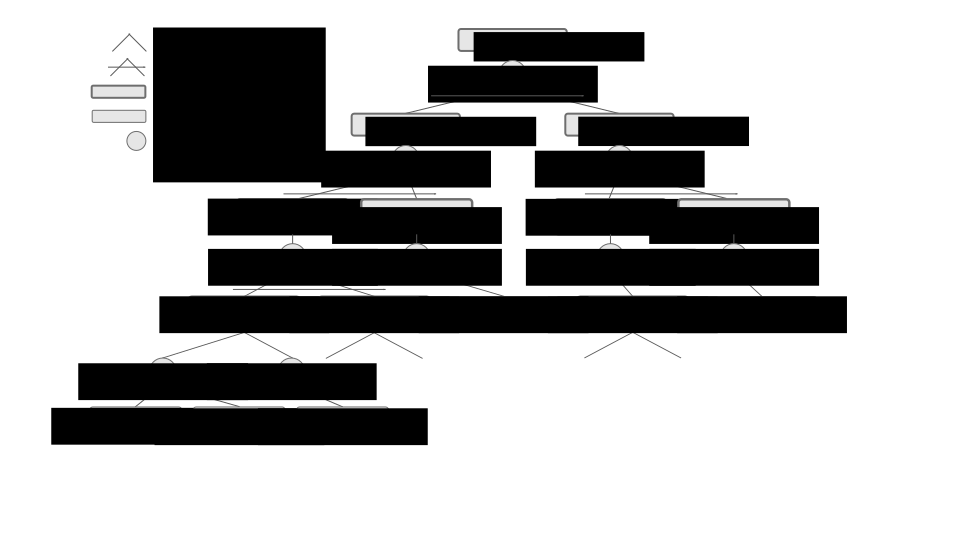
\includegraphics[width=\textwidth]{figures/chapter6/domain.png}
\caption{\label{fig:chap6_domain} The  domain of the high-level task \textit{PrepareMeal}. It is used by the planner (HATP) to elaborate a Human-Robot shared plan through a context-based decomposition and parameter instantiation process (which vegetable V, which knife K, ...) including the selection of which agent A (Tony the human, or PR2 the robot) abstract tasks and/or primitive tasks will be allocated.}
\end{figure}

Given an initial world state and an initial task to decompose, a planner such as HATP elaborates a plan through successive decompositions from the initial task and respecting the constraints issued by the initial world state. A resulting plan is a sequence of primitive tasks. The planner thus tries to recursively select a decomposition for each abstract task encountered until it reaches primitive tasks. Besides, the planner has to ground every argument of the tasks into entities of $\Abox$ (the Abox of the knowledge base $\kbs$) while respecting constraints regarding their types.

\subsubsection{The semantic and episodic knowledge bases}

The semantic knowledge base $\kbs$ is still an ontology as described earlier. The episodic knowledge base $\kbe$ is a timeline also called datebase~\cite{allen_1983_maintaining}. It maintains temporal reference for every fact that varies in time. Representing only the changes, we can assume that a fact holds between two changes.

We defined it as a pair $\kbe = ( \{ \langle \relation, \tau \rangle \}, \{ \langle \taction, \tinterval \rangle \} )$. The first element is a set of time-stamped relations like a classical datebase. The second element aims at representing the performed tasks. It is a set of pairs with $\taction$ an instance of a task and $\tinterval$ a temporal interval composed of two numerical values. The tasks defined in $\kbe$ are also represented as entities of $\kbs$ ($\taction \in \indivset$). Since they are semantically represented in $\kbs$ we can, inter alia, retrieve their types or arguments.

\begin{figure}[h!]
\centering
\includegraphics[scale=0.55]{figures/chapter6/ke.png}
\caption{\label{fig:chap6_ke} An example of timeline. In blue the performed tasks with their intervales and in red the relations changes.}
\end{figure}

Since we address HRI applications, in the same way, it has been done previously with the semantic knowledge base, we consider that the robot maintains a semantic and episodic knowledge base per human it is interacting with ($\kbs^{Hi}$ and $\kbe^{Hi}$ ) in addition to its own ($\kbs^{R}$ and $\kbe^{R}$). While the robot's own knowledge base is its personal truth, the agents' knowledge bases represent its estimation of the knowledge of its human partners.

\subsection{The knowledge gathering scheme}

We give now an overview of how the three knowledge bases are interconnected and how the semantic and episodic ones are updated. A minimal robotic architecture allowing the gathering of the necessary information is represented in Figure~\ref{fig:chap6_architecture}.

First of all, the task decomposition description stored as an HTN is parsed offline. We aim at extracting from it a semantic description of the tasks composing it (abstracts and primitives), their parameters, and their hierarchical links through the decompositions. All these descriptions are then stored into the ontology as classes and properties (dotted arrow on Fig.~\ref{fig:chap6_architecture}) in order to ground future executions traces.

Once the ontology initialized with a common ground of which the description of the planning domain is part, we can start the interaction. During the interaction, the situation assessment updates the semantic knowledge base of each agent with relations to the entities of the environment. Upon receipt of these facts, the semantic knowledge base temporally stamps them and stores them in the episodic knowledge base. Because it can also infer new facts thanks to the reasoning mechanisms, these inferred facts are also temporally stamped and stored in the episodic knowledge base\footnote{For now only the performed tasks will be used to generate the REs but we still wanted to have a more general scheme to understand the context in which we want to use it.}.

On request of the supervision module, the HTN planner takes its initial world state from the ontologies of the involved agents (1A) and generates a shared plan (1B). During the execution of the shared plan, the supervision describes the performed tasks semantically (detailed in the following subsection) (2A) and stamps them in the timeline (2B) with their respective begin and end times. While it knows the tasks performed by the robot, it needs to gather data from the episodic knowledge base of the human partner (2C), to monitor their tasks. The descriptions of the tasks are not stored in the episodic knowledge bases as not having any temporal mean. It would be nonsense to say that a task has a given parameter at a given time. We first describe it as having parameters on one side (2A) and then we describe when the task has been performed on the other side (2B). 

Upon a REG request from the supervision, the REG component explores the listener's both sematic and episodic knowledge bases (3) and returns the generated RE (4).

\begin{figure}[h!]
\centering
\includegraphics[scale=0.35]{figures/chapter6/architecture.png}
\caption{\label{fig:chap6_architecture} A "minimal" robotic architecture (on the base of the one of figure~\ref{fig:chap5_archi}) allowing to acquire and store the knowledge necessary to perform a REG using the past human-robot activities. The dotted arrow represents an offline acquisition. The other arrows are online interactions between the components. The numbering represents the execution order during the execution of a task.
The robot knowledge bases ($\kbs^{R}$ and $\kbe^{R}$) and the estimated mental states of its human partners ($\kbs^{Hi}$ and $\kbe^{Hi}$) are updated permanently by the Situation Assessment component which tracks changes in the environment and by the robot supervisor which controls robot planning and execution activities and monitors humans actions.}
\end{figure}

When the supervision component inserts the executed tasks in the semantic knowledge base, it thus creates a hierarchical execution trace (HET). The execution trace can differ from the initial plan since it can be the result of plan repair or re-planning steps within the same global task achievement. The HET thus contains the actions which have been performed and their link to the higher level of abstraction. No forgetting mechanism is concidered since we focus on "short" interactions (few hours) but adding one would avoid the knowledge bases to grow indefinitely and also represent the human forgetting mechanism. This could be for future work.

\subsection{Building the ontology}

The aim of the following representation is not for planning per se (since this is done by the human-aware task planner) but rather to allow to store and manipulate a description of the execution of the human-robot shared plans together with their hierarchical structure and the information provided by the situation assessment component.
What is provided is the hierarchical task decomposition together with a semantic description of the entities used as tasks parameters, their properties, and relations to other entities in the environment. Moreover, the descriptions presented below are automatically generated from a HATP domain and plan description~\cite{lallement_2014_hatp}.

\subsubsection{HTN in ontology}

An HTN represents the general knowledge about how to decompose high-level abstract tasks into executable primitive tasks. Since it is a piece of general knowledge, we represent it in the TBox and the RBox of the ontology. It allows instantiating the executed plan as individuals of the ontology.

\begin{figure}[h!]
\centering
\includegraphics[scale=0.4]{figures/chapter6/tbox_base.png}
\caption{\label{fig:chap6_tbox_base} The upper classes used to decribe an HTN.}
\end{figure}

We first define the classes and properties common to any HTN representation.
As illustrated on Figure~\ref{fig:chap6_tbox_base}, the upper class in the TBox to describe an HTN is \textbf{HtnConcept} from which inherit the classes \textbf{HtnDecomposition} and \textbf{HtnTask}. The HtnTask class is then refined into \textbf{HtnAbstractTask} and \textbf{HtnPrimitiveTask}.
The RBox is composed without hierarchy of the properties \textbf{hasDecomposition}, \textbf{hasSubtask}, \textbf{hasParameter}, and their inverse (e.g. $(hasParameter, isParameterOf) \in \invset$). The property $hasDecomposition$ links an abstract task to its decompositions. The property $hasSubtask$ links a decomposition to the tasks (primitive or abstract) composing it. The property $hasParameter$ links a task to any other entity.

To represent an HTN $\HTN$ we thus create in the ontology a new class $\class$ for each :
\begin{enumerate}
	\item primitive task $\task$ such as 
$\task \in \primtaskset \Leftrightarrow \class \in \classset \wedge (\class,\ HtnPrimitiveTask) \in H$.
	\item abstract task $\abstracttask$ such as $\abstracttask \in \abstaskset \Leftrightarrow \class \in \classset \wedge (\class,\ HtnAbstractTask) \in H$.
	\item decomposition $\decompo$ such as $\decompo \in \decomposet \Leftrightarrow \class \in \classset \wedge (\class,\ HtnDecomposition) \in H$.
\end{enumerate}

For each decomposition $\decompo$ we describe the following relations using annotation properties:
\begin{enumerate}
	\item A decomposition come from an abstract task such as $\abstracttask \in \tasknetwork \Leftrightarrow (\abstracttask,\ hasDecomposition,\ \decompo) \in \annotationset$
	\item A decompositions has sub-tasks such as $\decompo \in \decomposet \Leftrightarrow (\decompo,\ hasSubtask,\ \task) \in \annotationset$.
\end{enumerate}

To put it into practice , let us consider the abstract task \textit{PrepareVegetable} of the domain illustrated in Figure~\ref{fig:chap6_domain}. The generated OWL representation of the listing~\ref{lst:chap6_owl_domain} is first composed of the \textit{PrepareVegetable} class inheriting from the \textit{HtnAbstractTask} concept. Through the use of the property \textit{hasDecomposition}, we state that the task has two decompositions being \textit{PVDecomp\_A} and \textit{PVDecomp\_B}. To refine these decomposition, we than create the \textit{PrepareVegetableDecomp} class inheriting from the \textit{HtnDecomposition} concept. It will be use to group all the decomposition of the \textit{PrepareVegetable} abstract task. Considering the fisrt decomposition (\textit{d8} on Figure~\ref{fig:chap6_domain}), we create a new class for it. The class \textit{PVDecomp\_A} thus inherite of \textit{PrepareVegetableDecomp}. This decomposition is composed of two sub-tasks \textit{Cut} and \textit{Peel}.  However, to keep track of the fact that thay have to be executed in the context of the said decomposition we refine them. We define \textit{Cut\_PVDecomp\_A} and \textit{Peel\_PVDecomp\_A} respectively inheriting of the primitives tasks \textit{Cut} and \textit{Peel}. With the property \textit{hasSubtask} we then describe that \textit{PVDecomp\_A} has two sub-tasks \textit{Cut\_PVDecomp\_A} and \textit{Peel\_PVDecomp\_A}.

Even if a task is used several times in the same HTN, it will be described only once.

\begin{lstlisting}[frame=single, basicstyle=\scriptsize\ttfamily, label={lst:chap6_owl_domain}, caption={Description of the abstract task PrepareVegetable and one of its decomposition in the OWL language using the Turle syntax.},captionpos=b, style=OwlTurtle]
:PrepareVegetable rdf:type owl:Class ;
                  rdfs:subClassOf :HtnAbstractTask ;
                  :hasDecomposition :PVDecomp_A ;
                  :hasDecomposition :PVDecomp_B .

:PrepareVegetableDecomp rdf:type owl:Class ;
                        rdfs:subClassOf :HtnDecomposition .

:PVDecomp_A rdf:type owl:Class ;
            rdfs:subClassOf :PrepareVegetableDecomp ;
            :hasSubtask :Cut_PvDecomp_A ;
            :hasSubtask :Peel_PvDecomp_A .

:Cut_PvDecomp_A rdf:type owl:Class ;
                rdfs:subClassOf :Cut .
\end{lstlisting}

In the latter description we have only represented the hierarchy of the tasks. We now need to specify the parameters of each task. They are represented using the upper property \textit{hasParameter}. At the difference to se ones used to describe the hierarchy, these aim to be used to instantiate executed tasks. Indeed, this property is first refined into several ones, being \textit{hasParameter.i} with $i \in \mathbb{N}$. This refinement level describes the position of each parameter in the tasks arguments list. We thus have hasParameter.0 the property for the first parameter of an argument list, hasParameter.1 the property for the second one, etc. These refinements are independent of the translated HTN.

\begin{figure}[h!]
\centering
\includegraphics[scale=0.4]{figures/chapter6/rbox_params.png}
\caption{\label{fig:chap6_rbox_params} The properties hierarchy for the parameters of the \textit{Cut} task.}
\end{figure}

Each of these properties is then refined and specified for every task of the HTN to describe. This second specification aims at representing the parameters with their name in the task parameters list, their position isn the parameter list, and the type of entities they can be bounded to. Taking the example of the primitive task \textit{Cut} of Figure~\ref{fig:chap6_domain}, the generated description is presented in listing~\ref{lst:chap6_owl_params}. The parameter \textit{A} of the \textit{Cut} task is at position 0 of the parameter list. We thus define the property \textit{Cut\_hasParameter.A} as a refinement of the property \textit{hasParameter.0}. The resulting hierarchy is illustrated on Figure~\ref{fig:chap6_rbox_params} pour the parameters of the \textit{Cut} task. The parameter \textit{Cut\_hasParameter.A} aims at representing the agent performing the task. Consequently, the property has to link an \textit{Cut} task to an agent. We represent it respectively with the domain and the range of the property. The same process is performed for every parameter of each task.

\begin{lstlisting}[frame=single, basicstyle=\scriptsize\ttfamily, label={lst:chap6_owl_params}, caption={Description of the \textit{hasParameter} property specifications for the parameters (resp. the agent performing the task, the cut vegetable, and the used knife) of the \textit{Cut} primitive task in the OWL language using the Turle syntax.},captionpos=b, style=OwlTurtle]
:Cut_hasParameter.A rdf:type owl:ObjectProperty ;
                    rdfs:subPropertyOf :hasParameter.0 ;
                    rdfs:domain :Cut ;
                    rdfs:range :Agent .

:Cut_hasParameter.V rdf:type owl:ObjectProperty ;
                    rdfs:subPropertyOf :hasParameter.1 ;
                    rdfs:domain :Cut ;
                    rdfs:range :Vegetable .

:Cut_hasParameter.K rdf:type owl:ObjectProperty ;
                    rdfs:subPropertyOf :hasParameter.2 ;
                    rdfs:domain :Cut ;
                    rdfs:range :Knife .
\end{lstlisting}


\subsubsection{HET in ontology}

\section[REG algorithm modifications]{Modifying the REG algorithm to support the past experiences}

\section{Results}

\subsection{One execution trace for five reffering expressions}

\subsection{The impact of the extention on the performances}

\section{Adapting the verbalization algorithm}
\ifdefined\included
\else
\setcounter{chapter}{7} %% Numéro du chapitre précédent ;)
\dominitoc
\faketableofcontents
\fi

\chapter{Moving forward binary relations in the REG}
\minitoc

The contribution presented in this chapter is a preliminary work aiming to consider the limitations encountered by the contribution of the previous chapter. The presented method has been implemented but not tested with an integration of other components. This section deviates a little from the field of HRI to be more anchored in artificial intelligence. However, the ability to generate entity referencing in a more generic way is paramount for a robot to interact with humans. 

\section{Introduction}

Representing the whole complexity of the knowledge composing our world into a machine-readable language is a central issue in artificial intelligence. Coming from the Semantic Web, we saw that the use of an ontology through RDF-based languages succeeded in establishing itself in the field of artificial intelligence and therefore robotics. Although, what is often viewed as a limitation of ontology is its capability to only represent unary and binary relations. Binary relations such as \textit{"Sean Connery has the British nationality"} are described through the form of triples \textit{(sean\_connery, hasNationality, british)}. Unary relation such as \textit{"Sean Connery is an actor"} can them be transformed into binary relation through the addition of dedicated predicates \textit{(sean\_connery, isA, Actor)}. However, the description of more complex relations involving more than two entities is must more challenging using such representation.

Taking the example of Sean Connery\footnote{In the case you do not know who is Sean Connery feel free to take another actor that you like but you will have to adapt the entire example. Good luck.}, f we want to refer to him\footnote{Obviously we want to refer to him without his name since we consider a person having recognized himself in the previous note.}, we could state that he is the actor playing the role of James Bond. However, other actor played this role. We could also say that he is the actor playing in the film Gold finger but once again others do. We could finally explain that he is the actor playing the role of James Bond and playing in the film Gold Finger. However, limiting us to the use of binary relations modify the exact information. A more accurate description would be that he is the actor playing the role of James Bond in the film Gold Finger. Here we see the necessity of relations involving more than two entities. In our example, we need to link the three entities that are the actor "Sean Connery", the role "James Bond", and the film "Gold Finger". Together, they describe a performance. Without being explicitly linked all three theses information would not represent the performance. Moreover, without these links, we could give an explanation such as the actor playing the role of James Bond and playing in the film Rising Sun. Both information is true but does not make sense together.

To refer to an entity, being an object or an agent, such complex relations could be useful but have to be managed carefully to keep the link between each binary relation composing it. In the light of this consideration, we can observe that the description of past agent tasks used in the previous chapter is based on the same principle. Where we refer to Sean Connery through his role and the film he plays in, we have described the knife through the vegetable it has been to cut and the agent having used it. However, depending on the context of the conversation, is it not always necessary to use all the binary relations of such a complex one. We may need only one. Trying to list the actors having the honorific title of "Sir", the referring expression \textit{"The man having played James Bond"} could be sufficient. In the same way, to designate the knife, the sentence \textit{"The knife you cut with"} could also be sufficient in some context.

In this chapter, we will try to generalise the REG algorithm to deal with non-binary relations and pass over the limitations of the previous chapter. The algorithm has to be more generic should no more have any apriori of concepts and properties of the used ontology.
First, we review the literature concerning the representation of non-binary relation in the ontology. Then, we define what we will call a Compound Relation and how we can represent it. The modified algorithm is then detailed before ending with an efficiency comparison regarding the original version and the extended one.

\section[Related work]{Related work: A richer knowledge representation with n-ary relations}

A fundamental feature of relations is their \textbf{arity}. It is the number of individuals they involved~\cite{giunti_2019_representing}. In this sense, unary relations involved only one entity while binary relation involves two entities\footnote{The entities involved in a relation do not have to be distinct. If the same entity is used twice in the same relation the relation is still a binary relation}. What interest us here is n-ary relations with arity $n > 2$.

Well before being treated for ontology used that it is in RDF or OWL, several approaches have been proposed in the field of Artificial Intelligence through the use of semantic network\footnote{Here we close the loop with the hypothesis by Collins and Quillian of the structure of the semantic memory to be like a semantic network.}~\cite{brachman_1979_epistemological, sowa_2014_principles}. Deliyanni and Kowalski~\cite{deliyanni_1979_logic} were the first to explicitly treat the representation of n-ary relations with arity $n > 2$. They propose a semantic network composed of an element representing the relation itself. In this way, they have represented the assertion "\textit{John gives the book to Mary}" with five node and four arrows as illustrated in figure~\ref{fig:chap7_sem_net}. The central node \textit{el} allow linking the four elements of the assertion using only binary relations. The approach is tody know as \textbf{relation reification} and has been used in many applications~\cite{gangemi_2008_norms, welty_2006_reusable}.

\begin{figure}[ht!]
\centering

\includegraphics[scale=0.4]{figures/chapter7/semantic_net.png}
\caption{\label{fig:chap7_sem_net} The semantic network used to represent the assertion "\textit{John gives the book to Mary}". The element \textit{el} is used to represent the global event.}
\end{figure}

The general idea used in all the proposed approaches since Deliyanni is thus the creation of a \textbf{relation-class} that is instantiated to represent the n-ary relation. Then $n$ binary relations are created to link the $n$ entity to the relation-class instance. For a more global view of the different proposed patterns, you can refer to the survey~\cite{gangemi_2013_multi}.

For the use in ontology, no standard pattern has been approved by the W3C for the moment. However, a Working Group Note has been proposed for the standardisation of such relations in RDF and OWL~\cite{w3c_2006_defining}. In the note, two patterns are introduced with two variants for the first one.

The first pattern is based on the introduction of a new class for relation and works in the exact same way of the relation reification as illustrated in Figure~\ref{fig:chap7_w3c_p2}. The class \textit{Purchase} is a relation-class and its instance \textit{purchase\_1} is link the entities of the relation. Such pattern is said to be \textbf{without subject} as all the relation are oriented from the relation-class instance to the other entities.

\begin{figure}[ht!]
\centering
\includegraphics[scale=0.4]{figures/chapter7/w3c_p2.png}
\caption{\label{fig:chap7_w3c_p2} Ontological pattern 1 without subject proposed by the W3C Working Group. The describe assertion is "John buys a "I, robot" from books.com for \$15".}
\end{figure}

A variation of the first pattern is illustrated in Figure~\ref{fig:chap7_w3c_p1}. This variation is said to be \textbf{with subject}. The assertion described here is "Christine has a tumor with high probability". Here the subject of the relation is Christine. It is represented in the pattern by a relation oriented from Christine to the instance of the relation-class while the others are in the usual orientation. Such variation can be reproduced with the previous one by defining inverse relations. Defining the relation \textit{isBuyer} and \textit{isObject}, either John or the book can be the subject of the relation represented by \textit{purchase\_1}.

\begin{figure}[ht!]
\centering
\includegraphics[scale=0.4]{figures/chapter7/w3c_p1.png}
\caption{\label{fig:chap7_w3c_p1} Ontological pattern 1 with subject proposed by the W3C Working Group. The describe assertion is "Christine has tumor with high probability".}
\end{figure}

The second pattern aims at representing lists. With the previous pattern, it is assumed that the properties involved in the binary relation are only used once to identify uniquely each element of the relation. Wanting to represent the assertion "United Airlines flight 3177 visits the following airports: LAX, DFW, and JFK" the first pattern would be not adapted. With this other pattern, we create several instances of the relation-class each linked to the next and to an entity of the n-ary relation as illustrated in Figure~\ref{fig:chap7_w3c_p3}. Because one of the binary relations go from an entity of the relation to an instance of the relation-class, it is said to be with subject. This second pattern is dedicated to the description of lists.

\begin{figure}[ht!]
\centering
\includegraphics[scale=0.4]{figures/chapter7/w3c_p3.png}
\caption{\label{fig:chap7_w3c_p3} Ontological pattern 2 with subject proposed by the W3C Working Group. The describe assertion is "United Airlines flight 1377 visits the following airports: LAX, DFW, and JFK".}
\end{figure}

\section{Through the use of coumpound relations}

In the rest of the chapter, we consider the n-ary relations with arity $n > 2$ under the name \textbf{Compound Relations} (CR) because of the composition of binary relations to represent them on the principle of reification. The term relation will be used to speak about binary relations. We first define what is a CR in link with the ontology definition and on the base of the first pattern without subject, proposed by the Working Group Note. Then, we present an algorithm to pre-process them with the objective to facilitate their use in the REG algorithm.

\subsection{Defining a compound relation}

To define the structure of a Compound Relation we take the example of the purchase made by John on the website book.com to buy the book "I, Robot" at 15\$. This statement is graphically represented in Fig.~\ref{fig:chap7_cr}a and the underlying pattern in Fig.~\ref{fig:chap7_cr}b. To represent the compound relation, we start by creating a virtual entity (the instance of the relation-class) that will be the common link for all the relations involved in the compound relation. We call this instance entity the \textbf{Compound Entity} (CE). It is the dotted entity on Figure~\ref{fig:chap7_cr}, respectively $purchase\_1$ and $\indiv_c$. We consider as being part of the CR all the relations for which the CE is the subject: $(purchase\_1, has\_buyer, john)$. 

\begin{theorem} [Compound Relation]
\label{the:compound_relation}
For any $\indiv_c$ being a Coumpound Entity, a Coumpound Relation is defined by $R_c = \{ \relation_i\ |\  \relation_i = (\indiv_c, \property_i, \indiv_i), \forall \indiv_i \in \indivset\}$ meaning the set of relation composing it.
\end{theorem}

\begin{figure}[ht!]
\centering
\includegraphics[width=\textwidth]{figures/chapter7/CR.png}
\caption{\label{fig:chap7_cr} The graphical representation of compound relations. The dotted entity at the center of each representation is the so-called compound entity. The outgoing edges are the properties involved in the compound relation. The entering and faded edges are the corresponding inverse properties if any. The compound relation a) describe the purchase made by \underline{John} on the website \underline{book.com} of the book \underline{"I, Robot"} at \underline{15\$}. The compound relation b) is the underlying pattern of the previous example.}
\end{figure}

Regarding the previous definition, because any entity of an ontology could be considered as a CE, many set of relations without a real link could be considered as a CR. To solve it, we could define an upper class common the all the CE, meaning the upper \textit{RelationClass}. However, what better defines a CR is that to speak about one of its involved entities through it, we have to use other relation of the CR. In other words, to speak about Sean Connery using the role of James Bond, we have to speak about "Gold Finger" rather than "Murder on the Orient Express" because even if he played in both films, he played the said role only in the first-mentioned film. At the difference, the relation representing his nationality can be used independently to other relations. To represent this verbal link, Giunti et .al \cite{giunti_2019_representing} introduce an \textit{parametric pattern} on top of n-ary relations (Compound Relations). Their parametric pattern for the purchase example is the following : \textit{"() bought a () from () for ()"}. While as humans we easily identify the place of each entity in the pattern, it is a more complex task for machines. This choice of pattern is explained by their complex representation where they assign a position to each involved relation. Regardless of the representation complexity, this kind of pattern raises two issues. First, the pattern describes the entire CR and not aims to describe one of the involved entity through the CR (e.g. "\textit{() who bought a () from () for ()}"). Second, the pattern necessary involved all the relations composing the CR, while in the context of the REG, we could only need a part of them (e.g. \textit{"() who bought a ()}" if John is the only one who bought this book in the present context).

\subsection{A light way of representing the verbal link}

To represent the verbal link, we also choose to use parametric patterns, patterns for short. The patterns are defined as labels in the ontology. A CR can have multiple labels (i.e. patterns) depending on the subject of the pattern and the involved relations in the verbal link. The labels are not directly applied to the CE but to a class, it's inheriting. This means that all the entities inheriting from a class having its labels respecting the pattern are CE. In a way, we define here a relation-class but one the only base of labels.

\begin{theorem} [Compound Entity]
\label{the:compound_entity}
Given $\omega$ being a pattern, an entity $\indiv_c$ is a Compound Entity iif $\exists \class \in \classset | (\indiv_c, \class) \in \inheritset \land \omega \in \tlabel{(\class)}$
\end{theorem}

An advantage of this solution is that we do not define any new specific concepts or properties in the ontology meaning that any pre-existing ontology can be updated to be used in the REG process with CR only by adding labels. Our patterns have the following form : $\{?\property_4\}\ bought\ on\ \{\property_3\}\ by\ \{\property_1\}$. This pattern directly integrates the properties which can be used to form the relations composing the CR.

Given a compound entity $a_c$ with the previous label, to generate a referring expression using it, the place-holder $\{\property_3\}$ should be replaced by a referring expression of an entity $\indiv_i$ where $\indiv_i$ is the object of a triple $(\indiv_c,\ \property3,\ \indiv_i)$. Because we assume that a property can only appear once in a CR, we know that there is only one such object $\indiv_i$. In our example, we have $\indiv_i = \indiv_3$ for the $a_c$ CE.
In this way, without predefined order, an algorithm can easily replace the place-holders by the RE of the entities $\indiv_i$ of the relations $(\indiv_c, \property_i, \indiv_i)$ of the CR.

Since we are in the context of REG, the CR will be used as a reference to one of the entities involved in the CR. This specific entity is called the \textbf{subject entity} of the CR. 
For a subject entity to exist, an inverse property $\overline{\rm \property_i}$ must exists in the way that $(\property_i, \overline{\property_i}) \in \invset$ and $\relation_i = (\indiv_i, \overline{\property_i}, \indiv_c) \in \relationset$. If $\indiv_i$ is the subject entity, $\property_i$ is thus the \textbf{subject property} of the CR and is prefixed with a question mark in the pattern. In the example of Figure~\ref{fig:chap7_cr}, only $\indiv_1$ and $\indiv_4$ (resp. John and the book) can be subject of the CR. In other words, only these entities can be referred through the use of this CR. Among all the labels available to speak about the CR, the usable ones to speak about an entity are the ones for which the corresponding property is the subject property (i.e. prefixed by a question mark in the patterns). This choice to not consider the first in the pattern has been made to be adapted to any language. Among the possible labels of List.\ref{lst:chap7_john_labels}, the patterns L1 to L5 could thus be used as a reference for $\indiv_4$ (the book in our example) while the patterns L6 and L7 could be used as a reference for $\indiv_1$ (John in our example).

\begin{lstlisting}[frame=single, caption={ A part of the label set of the purchase compound relation.}, label={lst:chap7_john_labels}, captionpos=b, style=Labels, mathescape=true]
L1 - {?$p_4$} bought on {$p_3$} at {$p_2$}
L2 - {?$p_4$} bought by {$p_1$}
L3 - {?$p_4$} bought on {$p_3$} by {$p_1$}
L4 - {$?p_4$} bought at {$p_2$} on {$p_3$} by {$p_1$}
L5 - {$?p_4$} bought at {$p_2$} by {$p_1$}
L6 - {$?p_1$} who bought {$p_4$}
L7 - {$?p_1$} who bought {$p_4$} on {$p_3$}
\end{lstlisting}

\subsection{A strategy to explore compund relations}

In a graph exploration, an important parameter to avoid a combinatorial explosion is the branching factor. For the REG problem, an advantage of CR is that once we introduce a CR in the search algorithm we can directly know the relations involved in it. In this sub-section, our goal is thus to analyze the labels in the way to define the order in which the relations of the CR will be explored by the upper algorithm. By doing so, we will reduce its branching factor and thus avoid any combinatorial explosion of the REG algorithm.

\subsubsection{A naive strategy to explore compound relations}

Suppose we want to refer to the entity $\indiv_4$ using the compound relation embodied by the compound entity $\indiv_c$ of Figure~\ref{fig:chap7_cr}. This is made possible by the triplet $(\indiv_c,\property_4,\indiv_4)$ in the knowledge-base and its inverse $(\indiv_4, \overline{\property_4}, \indiv_c)$. The listing~\ref{lst:chap7_john_labels} presents some alternative ways in which we can verbalise entities through the CR. In order to refer $\indiv_4$, we can only use the ones where $\property_4$ is the subject property. Thus the labels L1 to L5 are the only ones that we can use. The parts of the compound relation used by labels L1 and L3 are illustrated in Figure~\ref{fig:chap7_cr_part}.

\begin{figure}[ht!]
\centering
\includegraphics[scale=0.4]{figures/chapter7/CR_part.png}
\caption{\label{fig:chap7_cr_part} The parts of the compound relation used in the label patterns L1 (a) and L3 (b).}
\end{figure}

What interest us in these labels are the properties because it is they that will form the relations to explore. From the patterns in listing~\ref{lst:chap7_john_labels}, we know that we can use label L1 to verbalize the triple set \textit{\{($\indiv_c$,$\property_4$,$\indiv_4$) ($\indiv_c$,$\property_3$,$\indiv_3$) ($\indiv_c$,$\property_2$,$\indiv_2$)\}} and label L2 to verbalise the triple set \textit{\{($\indiv_c$,$\property_4$,$\indiv_4$) ($\indiv_c$,$\property_1$,$\indiv_1$)\}}. On the other hand, other combinations of triples involving $a_c$ cannot be used to refer to $\indiv_4$. Therefore, we can see each label usable to refer $\indiv_4$ as a set of properties and the collection of usable labels as a family of sets. In our example, the family of sets over S is the collection:

\begin{align*}
 F\ =\ \{\{p_2\ p_3\ p_4\},
\{p_1\ p_4\},
\{p_1\ p_3\ p_4\},
\{p_1\ p_2\ p_3\ p_4\},
\{p_1\ p_2\ p_4\}\}
\end{align*}

From there, our goal is to create a search-tree that will conduct the exploration of the different labels of a CR through the exploration of the properties composing them. This search-tree has few constraints:
\begin{enumerate}
	\item The tree must be composed of a single root.
	\item All the descendants of a node have a common prefix of the property associated with that node. In this way, the search-tree is more precisely a trie, also called prefix tree.
	\item Walking through the tree from its root, we recompose all the subsets of the family $F$.
	\item The width of the tree must be as small as possible.
\end{enumerate}

A naive solution not minimizing the width of the tree is represented in Figure~\ref{fig:chap7_naive}a) for the purchase example. We consider the root $\property_4$ and create a branch per label. The resulting width is five. On the Figure~\ref{fig:chap7_naive}b) we merge the node representing the same property at an equivalent level. It reduces the branching factor for the beginning of the exploration by the global width is the same. Switching the elements $p_2$ and $p_3$ for L4 and keeping the merging principle, we can see in Figure~\ref{fig:chap7_naive}c) that the width of the trie can be reduced to four. An advanced algorithm to build the graph could thus reduce the width of the trie.

\begin{figure}[ht!]
\centering
\includegraphics[width=\textwidth]{figures/chapter7/naive.png}
\caption{\label{fig:chap7_naive} Two naive trie representations of the family of subsets extracted from properties involved in the label patterns. The trie a) considers the subject property as the root of the tree and creates a branch for each label pattern respecting the order of apparition of the properties. The trie b) takes the same construction rule as the a) but merges the common children of each node. The trie c) is the same principle of b) but the elements $p_2$ and $p_3$ have been switched for L4. While the two first tries have a width of five, the last has a width of four.}
\end{figure}

\subsubsection{Advanced strategy to explore compound relations}

To find a strategy to create a trie minimizing the width, we first have to study the characteristics of the family of sets.
The first axiom that we can do on the subsets of our family is that they are neither totally ordered, as we can explore their element in any order, or partially ordered, as we can not compare their members. Therefore, we cannot use the tools of the order theory such as the Hasse diagram. Taking a look at mathematical approaches of tree-representation of set families~\cite{bui_2008_tree}, we face the problem that our set family does not respect some essential properties. For each pair $(A, B)$ of sets of $S$, we can not ensure that one of the following rules is true : $A \cap B \neq \emptyset$, $A \cap B \neq A$, or $A \cap B \neq B$. This means that we cannot ensure that each pair of sets are either disjoint or related by containment. Wherefore, our family $F$ is not a laminar set family.
Moreover, for each pair $(A, B)$ of sets of $S$, we can not ensure that their intersection is non-empty ($A \cap B \neq \emptyset$), neither that their difference are non-empty ($A \setminus B \neq \emptyset$ and $B \setminus A \neq \emptyset$). Wherefore, our family $F$ is not a cross-free or an overlap-free family but it does not mean that it is an intersecting and crossing family.

To limit our problem, we do a first assumption. Because the subject property $\property_s$ is the one having introduced the CR, we can assume that this property has already been selected among the others. Moreover, it will always be the common element of all the sets of the family. We thus consider it as the root node of the exploration tree and remove it from every set of the family $S$ giving a new family:

\begin{align*}
S' = \{A\ |\ A = X \setminus \property_s,\ \forall X \subseteq S\}
\end{align*}

From there, we need to find the child nodes of the root in a way to minimize their number and that every subset of $S'$ has at least one of their element attached to one of the child nodes. This sub-problem is a specification of the Hitting Set problem. It is defined as follows. Giving $F = \{S_1,S_2,...,S_m\}$ the collection of subsets of $S$ (i.e. $S_i \subseteq S, \forall i$) and a natural number $k \in \field{N}$, we want to know if exists $S' \subset S$ where $|S'| < k$ such that $S_i \cap S' \neq \emptyset, i = 1,2,...,m$. In our case, we are searching $k$ as to be as small as possible. In some way, the Hitting Set problem can be seen as a Set Covering problem, shown to be NP-complete~\cite{karp_1972_reducibility}. To avoid any combinatorial explosions, we thus propose a greedy algorithm.

Giving a node $n_i$ of the tree and it related family of set $S$, the quantity $|\{S_j \in S ~|~ x_i \in S_j \}|$ is the frequency of the element $x_i$ in $S$. Among the elements of the universe of the current node $n$, we select $x_{max}$, the element with the highest frequency and create a child node with it. The family related to this new node is computed with the equation~\eqref{eq:chap7_child_family} and the family related to the current node is updated with the equation~\eqref{eq:chap7_node_family_update}. These steps are repeated while $S$ is non-empty to create all the children of the current node and all this process is repeated for each created child nodes until it is possible.

\begin{equation}
S' = \{S_j \setminus x_{max}, S_j \cap \{x_{max}\} \neq \emptyset, \forall S_j \in S\}
\label{eq:chap7_child_family}
\end{equation}

\begin{equation}
S \leftarrow \{S_j, S_j \cap \{x_{max}\} = \emptyset, \forall S_j \in S\}
\label{eq:chap7_node_family_update}
\end{equation}

The tree resulting from this process is represented in Figure~\ref{fig:chap7_advanced} for the purchase example. In the root node with the property $p_4$, the element with the highest frequency is $p_1$. We thus create a child node with this property and create its family. Updating the family of the root node, the family only contains the set $\{p_2, p_3\}$. Both having the same frequency, one is chosen over the other, here $p_3$, and we create a new child node. After an update of the family of the root, it will be empty and all the children of the root have been created. The process is repeated for the two created nodes.

\begin{figure}[ht!]
\centering
\includegraphics[scale=0.45]{figures/chapter7/advanced.png}
\caption{\label{fig:chap7_advanced} The trie with reduced width, representing all the labels of a compound entity in terms of involved properties. Each node is a property to explore. Attached to each node is the family of subsets that has to be decomposed. An empty set in a family related to a node (in red) signified that one of the initial subsets is fully represented in the trie meaning that all the properties of a pattern will be explored by reaching this node. The width of the trie is three against five for the naive version.}
\end{figure}

In the following, such search-tree will be referred to as a Compound Tree (CT). Taking a part of it (i.e. taking one of its nodes as a local root) gives a sub-CT.

\section{REG with compound relations}

Thanks to the CE labels analyse, we have created a search-tree to lead the exploration of CR in the REG algorithm. In this section, we present the modification we made to use CR in the REG algorithm. The core of the algorithm based on the Uniform Cost Search algorithm is unchanged and is recalled in algorithm~\ref{alg:chap7_ucs}.

\begin{algorithm}[!ht]
\caption{Uniform-Cost Search algorithm for Referring Expression Generation}
\label{alg:chap7_ucs}
\begin{algorithmic}
\Function{UCS\_REG}{$problem$} 
    \State $node\leftarrow$ a node with RE = \textsc{create-initial-re}(\textit{problem}.context), \textit{cost} = 0
    \State $frontier\leftarrow$ a priority queue of nodes ordered by their \textit{cost}
    \State $frontier\leftarrow$ \textsc{INSERT}($node$, $frontier$)
    \State $explored\leftarrow$ an empty set
    \Loop
        \If{\textsc{empty}($frontier$)} 
        	\State \Return failure
        \EndIf
        \State $node\leftarrow$ \textsc{pop}($frontier$)
        \If{\goaltest($problem$, \toquery($node$))} 
        	\State \Return \textsc{SOLUTION}($node$)
        \EndIf
        \State add $node.RE$ to $explored$
        \ForAll{$addition$ in \additions($node$)}
            \State $child \leftarrow \createchild(node, addition)$
            \If{$child.RE$ is not in $explored$ or $frontier$}
            	\State $frontier\leftarrow$ \textsc{INSERT}($child$, $frontier$)
            \EndIf
        \EndFor
    \EndLoop
\EndFunction
\end{algorithmic}
\end{algorithm}

\subsection{Exploring the compound relations}

At the difference of the tasks descriptions of the previous chapter, the current algorithm can not have any prior knowledge about the relations leading to the use of CR. A CR can only be discovered if a relation introduces a CE. However, an entity can be said to be a CE only thanks to the labels of one of its upper class. With regard to this information, we cannot have any function dedicated to the addition of CR and each newly introduced entity in a candidate RE has to be tested to assess if it is a CE or not.

The analyse of the entities' labels and their usable classes, meaning their upper classes having labels, is an already existing process in the REG algorithm. It is performed by the function $\typingadditions$ of algorithm~\ref{alg:typing_action}. It initially aims at satisfying the parlance need constraint. With some modifications, the $\typingadditions$ will be used to detect any newly introduced CE by testing if the labels of the usable classes are in the form of a pattern. If they are it returns the detected CE. To do so, the \textit{additions} are now composed of a relation to be added and a CE in one has been found.

Once CEs have been detected, we have to create a Compound Tree (CT) for each in order to lead the REG search process. To each node of the REG algorithm, in addition to the candidate RE and its associated cost, we introduce a map of CTs. This map link a CE involves in the candidate RE related to the node to its CT or one of its sub-CT. The management of these trees is done by the $\createchild$ that has been modified (see algorithm~\ref{alg:chap7_child}. If the addition introduces a new CE, we create it related CT\footnote{For performance gain, all created CT can be stored in a collection of CT in order to compute them only once even if the same CE is introduced in two disting branches of the UCS.}. Otherwise, with the function $\getsubtrees$ we test is the new relation corresponds to one of the branches of one of the CTs of the parent node. If it is, we take the sub-CT corresponding to the relation. Taking the entity $\indiv_c$ as introduced CE through the relation $(\indiv_4, \overline{\property_4}, \indiv_c)$, the CT of figure~\ref{fig:chap7_advanced} is first created. If in a second time the relation $(\indiv_c, \property_1, \indiv_1)$ is inserted, $\createchild$ would take the sub-CT having $\property_1$ as root.

\begin{algorithm}[H]
\caption{\label{alg:chap7_child} Child node function modified to use compound relations.}
\begin{algorithmic}
\Function{\createchild}{$addition$, $parent$} 
    \State \Return a node with
    \State RE = $parent$.RE $\cup$ $addition$.relation
    \State cost = $parent$.cost + $\costfunc(addition$.relation$)$
    \If{$addition$.CE}
    	\State CTs $\leftarrow$ INSERT($\createtree(addition$.CE$)$, $parent$.CTs)
    \Else
    	\State CTs $\leftarrow$ $\getsubtrees$($addition$.relation, $parent$.CTs)
    \EndIf
\EndFunction
\end{algorithmic}
\end{algorithm}

At this stage, we detect the introduction of CR and manage the CTs. The $\additions$ can now use the CTs to propose new additions. As describe with the algorithm~\ref{alg:chap7_additions}, we keep the two functions $typingadditions$ and $\differenceadditions$. We introduce a new function $\compoundadditions$ aiming to complete the CR having been started. For each CT of the node it propose the relation of the form $(\indiv_c, \property_i, \indiv_i) \in \relationset$ such that the properties $\property_i$ are the branches of the root of the CT related to $\indiv_c$. With the  CT of figure~\ref{fig:chap7_advanced}, the $\compoundadditions$ function would generate two addtions being $(\indiv_c, \property_3, \indiv_3)$ and $(\indiv_c, \property_1, \indiv_1)$.

\begin{algorithm}[htb!]
\caption{\label{alg:chap7_additions} The modified $\additions$ function modified to use compound relations. }

\begin{algorithmic}

    \Function{\additions}{$node$} 
        \State $sucess, additions\leftarrow$ \typingadditions($node$)
        \If{$sucess = True\ and\ additions \neq \emptyset$}
            \Return $additions$
        \EndIf
        
        \State $additions\leftarrow$ \compoundadditions($node$) \Comment{new introduced function}
        \State $additions\leftarrow additions\ \cup$ \differenceadditions($node$) 
        
        \Return $additions$
    \EndFunction
    
\end{algorithmic}
\end{algorithm}


\subsection{Determining a referring expression validity}

Going back to the original definition of the REG problem, a RE is valid if the parlance need is satisfied (theorem~\ref{the:parlance_need}), all the introduced variables can be intantiated (theorem~\ref{the:correct_intance}), and the variable representing the target entity can only be bound to the target entity (theorem~\ref{the:re_mini_validity}) for a minimal validity.

For the compound relations, their validity criteria is that we can use onr of their labels to speak about them. In other words, taking all the relations involving a given CE, we must be able to rebuild one of his family's sets. Each of its CR thus has to be complet (see theorem~\ref{the:cd_completion}).

\begin{theorem} [The CR completion]
\label{the:cd_completion}
A CR of family $S$ is said to be complet iif given its CE $\indiv_c$ we can create, from the set of relation $\mathcal{T}$ representing a candidate RE, a set $v = \{\property_i\ |\ (\indiv_c, \property_i, \indiv_i) \in \mathcal{T} \lor (\indiv_i, \overline{\property_i}, \indiv_c) \in \mathcal{T} \}$ such that $v \subset S$.
\end{theorem}

From a technical point of view, such constraint can be hard to compute for each node to be tested. However, during the creation of a CT, this information can already already known. During the CT creation, each time a child node is created with an empty set its family of sets, this means that a label of the CR is represented in its entirety at this node. On the figure~\ref{fig:chap7_advanced} the completed labels are represented by the red arrows. We can thus store this information in the CT nodes. Because during the REG search process we cut down these trees taking each time a sub-CT, we just have to test if each current root of the CTs of the node to test can represent a label or not. If all can, the candidate RE of the current node is valid regaring the CR completion.

\subsection{From tree to radix tree}

A limitation identified from the previous chapter was the addition of a single relation at each step while we can know that the candidate RE will not be valid because of the completion constraint. With the present method using multiple labels not involving all the relations, the limitation has been partially solved. In addition, thanks to the CT, the branching factor is limited and even if an addition does not lead to a valid RE, it will be used for several labels. However, in some cases, this limitation still appears. Considering the Compound Tree of figure~\ref{fig:chap7_advanced}. Starting from the root node $\property_4$, we can go to the nodes $\property_3$ and $\property_1$. While the node $\property_1$ create a complete CR and make a step toward another complete CR, the node $\property_3$ does not. It makes a step toward the single label $L1$ but does not complete it.

To solve this issue, we can use the radix tree structure, also called compact prefix tree. It consists of merging each node that is the only child with its parent if the parent node does not represent a valid label. In the example of figure~\ref{fig:chap7_advanced}, the node with the property $\property_2$ could thus be merged with its parent $\property_3$.

The major consequence of such modification is that the additions have to no more represent a single relation but a set of relations. Even if it makes the additions comparison harder to compute it reduce the overall branching factor. Keeping our example, if we add at once the relation involving $\property_2$ and $\property_3$ and that both introduce an anonymous entity, this means that at the next step the $\typingadditions$ function could type both at once. Where previously these additions would require four steps, and thus branching at each, with this solution it only required two.

\section{Results}

In this section, we present some result of the REG with compound relations. We start with the introduction example of Sean Connery's performance. Then we give performance measures using the setup of the previous chapter in order to assess the impact of the proposed modifications. 

\subsection{The actor playing James Bond}

For this simple test, we describe actor performance using the pattern of figure~\ref{fig:chap7_perf}. Both the actor and the film can be used as a subject of the CR thanks to the presence of inverse properties. The set of labels attached to the \textit{Performance} class is listed in listing~\ref{lst:chap7_perf_labels}. Three are available to describe the actor and two (equivalent) for the film.

\begin{figure}[ht!]
\centering
\includegraphics[scale=0.4]{figures/chapter7/perf.png}
\caption{\label{fig:chap7_perf} The compound relation patten used to discribe a performance of an actor with a role and a film.}
\end{figure}

\begin{lstlisting}[frame=single, caption={ The set of labels usable to discribe the performance compound relation.}, label={lst:chap7_perf_labels}, captionpos=b, style=Labels, mathescape=true]
L1 - {?perfHasActor} who played {perfHasRole} in {perfHasFilm}
L2 - {?perfHasActor} who played {perfHasRole}
L3 - {?perfHasActor} who played in {perfHasFilm}
L4 - {?perfHasFilm} in which {perfHasActor} play {perfHasRole}
L5 - {?perfHasFilm} in which {perfHasRole} is played by {perfHasActor}
\end{lstlisting}

We first create an ontology describing two performances. The performance \textit{perf\_sean} link the actor \textit{sean\_connery} with the role of \textit{james\_bond} and the film \textit{gold\_finger}. The second is \textit{perf\_craig} with \textit{daniel\_craig} in the role of \textit{james\_bond} and in the film \textit{casino\_royale}. The individuals representing the films and the roles have labels while the others do not. Running our algorithm on this ontology we get the result:

\begin{gather*}
(?0,\ isA,\ Actor),\\
(?0,\ isActorOfPerf,\ ?1),\\
(?1,\ isA,\ Performance),\\
(?1,\ perfHasFilm,\ gold\_finger)
\end{gather*}

Matching it the the ontology, the variable \textit{?0} matchs \textit{sean\_connery} and the variable \textit{?1} matchs the performance \textit{perf\_sean}. Adding the performance \textit{perf\_gert} linking the actor \textit{gert\_frobe} with the role of \textit{auric\_finger} and the film \textit{gold\_finger} the previous solution is no more valid. Running the algorithm on the new ontology, we get the result:

\begin{gather*}
(?0,\ isA,\ Actor),\\
(?0,\ isActorOfPerf,\ ?1),\\
(?1,\ isA,\ Performance),\\
(?1,\ perfHasFilm,\ gold\_finger),\\
(?1,\ perfHasRole,\ james\_bond)
\end{gather*}

With this simple example we see that with a single compound relation, the algorithm is able to find a solution by selecting the necessary information in it depending on the situation while keeping the link between each of them.

\subsection{The desciption of past activities as compound relations}

Since the presented algorithm is able to manage the past tasks description, we present a comparison in terms of execution time with both the original algorithm and the one using past tasks. To do so, take the knowledge base of the previous chapter containing two task description per entity inheriting from the \textit{Object} class. To be used with compound relations, we add a label to each class representing a task. The label involves the three parameters of the task. In this way, we reproduce the constraint to use all the parameters and at the same time take advantage of the radix-tree optimisations. The knowledge base is still managed using the Ontologenius system and not passing by the ROS services to not be impacted by the communication time in our measures.

The original algorithm has been run without the possibility to use relations toward task since it is not designed for this use. Its performance is our comparison point as we expect all algorithms to find the same solutions. For recall, the described tasks are designed in such a way to not help in the RE generation and but ourselves in the worst case. The measures of the percentage of entities referred over time for all three algorithms are represented in Figure~\ref{fig:chap7_compare} and reported on table~\ref{tab:reg_compare}.

\begin{figure}[h!]
\centering
\includegraphics[scale=0.5]{figures/chapter7/comparison.png}
\caption{\label{fig:chap7_compare} Comparison of the three algorithms regarding the percentage of successfully referenced entities over time using a logarithmic timescale. }
\end{figure}

With this setup, the current version performs slightly better than the previous one with an average resolution time of 4.17ms versus 5.53. It is however over the original version having an average resolution time of 1.08ms. This difference must be qualified by the exploration of CRs that the original one does not do. While the majority of the entities are referred in a comparable time with the previous version, we can still note that the more complex entity requiring six relations is now solved in 45.71ms versus 70.57ms previously.

An advantage of the current algorithm is that in the case no CRs are described the performance are the same as the original algorithm. At the difference, the previous version had an impact even if negligible. 

% chap 4
%count    77.000000
%mean      1.080750
%std       1.355236
%min       0.013237
%25%       0.193782
%50%       0.516371
%75%       1.322064
%max       6.405807

% chap 6
%count    77.000000
%mean      5.531283
%std       9.780631
%min       0.012952
%25%       0.509738
%50%       1.538461
%75%       5.968753
%max      70.577606

% chap 7
%count    77.000000
%mean      4.178141
%std       6.855033
%min       0.016902
%25%       0.438766
%50%       1.323878
%75%       5.447168
%max      45.716713
\ifdefined\included
\else
\setcounter{chapter}{8} %% Numéro du chapitre précédent ;)
\dominitoc
\faketableofcontents
\fi

\chapter{A robot in the mall: The MuMMER project}
\minitoc

This chapter is a sum-up of an article submitted to the  User Modeling and User-Adapted Interaction (UMUAI) Journal. This work has been achieved in collaboration with Amandine Mayima, Guilhem Buisan, Phani-Teja Singamaneni, Yoan Sallami, Kathleen Belhassein, and Jules Waldhart. In this chapter, we first give an overview of the European H2020 Project \acrfull{mummer}\footnote{\url{http://mummer-project.eu/}}, in the context of which the contribution of chapter~\ref{chap:3} was made. We then present the components developed by the LAAS-RIS team with a focus on the component in which I participated as well as their integration in a robotic architecture.

\section{Introduction}

In large scale, indoor environments, like museums, shopping malls, or airports, the presence of large interactive screens, maps, or signs underline the importance of providing information on itineraries. However, reading such maps can be challenging and some information can be missing like the location of the shops selling a given product. To bring such new information and help people to find their itinerary in large indoor environments such as shopping malls, robots can be used.

To study this challenge and the underlined Human-Robot Interaction requirement, in the context of the European H2020 Project \acrshort{mummer}~\cite{foster_2016_mummer}, we have developed and deployed a social service robot in one of the largest malls of Finland, Ideapark in the city of Lemp\"a\"al\"a. The resulting robot is able to chat with customers and guide them. The chatting has been brought by a partner of the project. The contribution of the LAAS-RIS team, and thus the focus of this chapter, was on the direction-giving task.

With a mall having approximately 1.2 kilometers of pedestrian streets and more than 150 shops, having a robot accompanying customers would be time-consuming. Taking inspiration from the mall employees, we chose to verbally describe the route while grounding it with pointing gestures. The robot can however move a few meters if needed. %Such a movement can be useful to improve the perspective sharing of landmark to better ground the route description.
The output of this project is a complete robot architecture that integrates a number of components. Each of them makes use of various models and decisional algorithms, all integrating explicitly human models.

First, we provide background information about robot guides and discuss how the human partner has been considered. Then, we present the human-human exploratory studies used to identify the required abilities for a guide robot. We then present the developed architecture and its components. We end this chapter with integration on a real robotic system with some detail on its deployment "into the wild".

\section{Related work}

A number of contributions have proposed robot guides, from the first museum guides \cite{burgard_1999_museum, siegwart_2003_robox, clodic_2006_rackham} to more recent robot guides in large areas \cite{bauer_2009_autonomous, triebel_2016_spencer}. A recent example is presented in \cite{chen_2017_robots}. The developed robot is able to accompany the customer to its destination, then to point at it. Another robot presented in \cite{gross_2009_toomas} can help the customer to find specific product among all the shops of a mall. Most of these works are focused on the navigation aspect of the task. It requires environment mapping, localisation, and social navigation due to the presence of many humans.

Where previous contributions were mostly focused on navigation, others have investigated the direction-giving task, meaning the fact to not accompany the customer but to describe the route to the goal. For example, \cite{cassell_2007_trading} describes an embodied conversational agent giving route directions using deictic gestures. Within the Robovie project, the ATR-IRC laboratories have developed a robot providing route description through the use of utterances and gestures, and have highlighted the importance of their timing~\cite{okuno_2009_providing}. Kanda et al. in \cite{kanda_2009_affective} and \cite{kanda_2010_communication} have divided the direction giving into two steps. First the robot point toward the direction to take, then it explains the full route. In addition, the robot can give recommendations for restaurants and shops. Finally, \cite{satake_2015_should} showed a complete architecture of an information-providing robot able to move around a square in a mall. It embedded a map, an ontology, a speech recognition system, a dialog manager, a localization module, and a people tracker. As in their previous works, the robot verbalized utterances and used deictic gestures to give route directions. Numerous other contributions can be found but, only a few of them propose full architectures for an autonomous direction-providing robot, the most complete one being the Robovie robot presented above. 

To the best of our knowledge, no system tackles the guiding-task by reasoning about the shared perspective. If the robot has to point a landmark not visible by the human at its current position, we want the robot to pro-actively propose to the human a pertinent placement. This is one of the basic bricks of our system and it is strongly linked to the key principles of Joint Action which involve the ability to establish and monitor joint attention~\cite{pacherie_2012_phenomenology}.

\section{Learning from exploratory studies}

To lead to robot abilities design and implementation, two human-human exploratory studies were conducted in collaboration with VTT Technical Research Centre of Finland. In addition to the current literature, it allows us to enrich our knowledge with effective route descriptions in the robot deployment environment.

The first pilot study consisted of a human guide providing route information. It consisted of one participant asking for shop directions to a guide working at the mall information booth. The analysis focused on gestures used to give guidance, the positions of the two protagonists in relation to the target shop and their interlocutor, and the gazes alternation. \cite{belhassein_2017_human} gave the first indications to consider resulting from this pilot study. Among these results, we can note a preference over the ipsilateral hand to the visual field of the target. This study also provides numbers of dialogue transcription use to study how guides effectively provide route description and give examples of descriptions.

\begin{figure}[ht!]
\centering
\includegraphics[scale=0.35]{figures/chapter8/human_guide.png}
\caption{\label{fig:chap8_human_guide} Picture from the second Human-Human study \cite{belhassein_2017_human}. Here, the guide is giving the route description to reach a given shop by pointing at it. The formation formed by the guide, teh customer, and the target were analyzed. }
\end{figure}

A second exploratory study was then carried out to focus on more complex situations. Among them, we can note situations with two customers requesting directions simultaneously, a customer requesting for two shops at the time, or someone interrupting an ongoing interaction. Once again the formations were analyzed. An example of such a formation seen during the study can be seen in figure~\ref{fig:chap8_human_guide}. The full results can be found in~\cite{Heikkilae_2018_where} and~\cite{heikkilae_2019_should}. Among these results, the study has shown that the guide usually points to the general location of the target first and in a second step explain and point the different stages of the route.

\section{The deliberative architecture}

\begin{figure}[ht!]
\centering
\includegraphics[width=\textwidth]{figures/chapter8/architecture.png}
\caption{\label{fig:chap8_architecture} todo. }
\end{figure}

\subsection{Environment representation}

\subsubsection{Geometric representation}

\begin{figure}[ht!]
\centering
\includegraphics[scale=0.15]{figures/chapter8/adream_base_m.png}
\caption{\label{fig:chap8_adream_base} todo. }
\end{figure}

\begin{figure}[ht!]
\centering
\includegraphics[scale=0.15]{figures/chapter8/ideapark_base_m.png}
\caption{\label{fig:chap8_ideapark_base} todo. }
\end{figure}

\subsubsection{Semantic representation}

\begin{figure}[ht!]
\centering
\includegraphics[scale=0.45]{figures/chapter8/zizzi.png}
\caption{\label{fig:chap8_zizzi} todo. }
\end{figure}

\subsection{Perceiving the partner}

\subsection{Generating route description}

\subsection{Planning a shared visual perspective}

\begin{figure}[ht!]
\centering
\includegraphics[scale=0.25]{figures/chapter8/grid_map.png}
\caption{\label{fig:chap8_svp_grid} todo. }
\end{figure}

\begin{figure}[ht!]
\centering
\includegraphics[scale=0.45]{figures/chapter8/svp.png}
\caption{\label{fig:chap8_svp} todo. }
\end{figure}

\subsection{Navigate close to the human}

\subsection{Executing and controling the task}

\section{Embody architecture in a physical robot}

\subsection{Pepper in Ideapark}

\begin{figure}[ht!]
\centering
\includegraphics[scale=0.15]{figures/chapter8/pepper_mall.png}
\caption{\label{fig:chap8_pepper_mall} todo. }
\end{figure}

\subsection{Pepper "in the wild"}
\ifdefined\included
\else
\setcounter{chapter}{9} %% Numéro du chapitre précédent ;)
\dominitoc
\faketableofcontents
\fi

\chapter{The Director Task: Assessing cognitive architectures}
\chaptermark{The director task}
\minitoc
\label{chap:9}

In this chapter, we propose a new psychology-inspired task, gathering perspective-taking, planning, knowledge representation with theory of mind, object manipulation, and Human-Robot communication. Along with a precise description of the task allowing its replication, we present a cognitive robot architecture able to perform it in its nominal cases. In addition, we suggest some challenges and evaluations for the Human-Robot Interaction research community, all derived from this easy-to-replicate task.

The contribution presented in this chapter is excerpted from our work, published in the proceedings of the RO-MAN 2021 conference~\cite{sarthou_2021_director}. This contribution closes this thesis and has been achieved in collaboration with other PhD students of the \acrshort{hri} team. Guilhem Buisan was concerned about the task planning part. Amandine Mayima worked on the supervision component. Kathleen Belhassein has designed the presented task with us giving her psychologist point of view to create a task on which user studies could be performed. The engineer Yannick Riou worked on the motion planning component allowing us to develop a task where the robot acts on its environment. My responsibility for this task has been the integration of my previous contributions about Ontology and the \acrshort{reg}. It has also been the opportunity to create an entire architecture extending the ones presented all along with this thesis and linked with the contributions of the team. Finally, I have contributed to the Situation Assessment component and on the Language understanding part.

The components related to my teammates will be briefly described to give an overview of the architecture. The newly introduced capabilities on which I work will be more detailed to explain the links I make between all my contributions, centred on the knowledge representation.

\section{Introduction}

Developing robotic architectures adapted to Human-Robot Interaction and thus able to carry out interactions in an acceptable way is still today a real challenge. The complexity comes, among other things, from the number of capabilities that the robot must be endowed with and therefore from the number of software components which must be integrated in a consistent manner. Such architectures should provide the robot with the capability to perceive its environment and its partners, to merge and interpret this perceptual information, to communicate about it, to plan tasks with its partner, to estimate the others' perspective and mental state, etc. Once developed, the evaluation of these architectures can be difficult because all these components are grouped into a single system. The tasks we usually want the robot to handle must highlight a maximum of abilities, while still being simple enough to be reproduced by the community. Moreover, we should be able to conduct user studies with it to validate choices regarding naive users.

Since a long term goal of the robotic field is to see robots acting in our daily life, many tasks and scenarios have been inspired by everyday activities. Even if these tasks offer a large variety of situations to be handle, since the human partner is not limited in his actions, they have the disadvantage of not highlighting some subtle abilities which are nevertheless necessary for good interaction.
The robot guide task \cite{satake_2015_should} in mall, museum, or airport, requires high communication skills to understand free queries (possibly involving chatting) and respond to them, whether to indicate a direction or to give advice. However, the perception needs can be limited due to the vast environments, as well as the perspective-taking needs due to the same perception of the environment by the robot and the human\footnote{For sure we can find some tricky cases where it could help but they do not reflect common situations.}. Finally, even if the human should contribute to the problem, with such a task the human partner is not necessarily an actor of the task and can just listen to the robot once their question is asked. Even if being in more constrained environments, bartender-like tasks~\cite{petrick_2012_social} have the same disadvantages. Indeed, the human is considered as a customer, and as such, the interaction with the robot is limited. The robot will never ask the human to help it for performing a task and its actions do not require coordination either full collaboration.

To involve the human partner in the task and requiring him to act with the robot, assembly-like tasks~\cite{tellex_2014_asking}\footnote{This task is not explicitly intended to be replicated by the community.} can be used. Nevertheless, in most cases, the human acts as an assistant rather than as a partner as full collaboration can be challenging to perform. The robot thus elaborates a plan and performs the assemble, then asks for help when detecting errors during the execution (e.g., when it cannot reach some pieces). Here the task leads to unidirectional communication. Moreover, because in such a task both the robot and the human have equivalent knowledge about the environment, it can be hard to design situations where belief divergence appears and thus perspective-taking would be required.

Scaling down an everyday task to transform it into a toy task around a table can reduce the task complexity and allow easy reproducibility. Moreover, it allows the robot and the human to work in the vicinity of each other, with smaller robots for example. With the toy version of the assembly task presented in~\cite{brawer_2018_situated}, the human is more involved in the task. They ask the robot to take pieces and to hold them to help them assemble a chair. Even if the communication is unidirectional, we could imagine inverting the roles to test different abilities. Moreover, communication implies objects referring with the use of various visual features about the entities. Even if both agents have the same knowledge about the environment, the communication is grounded according to the current state of the world. In this task, no decision has to be made by the robot but once again, inverting the roles could open other challenges.

To focus studies around perspective-taking and belief management, the Sally and Anne scenario, coming from a psychology test, has been studied in robotic~\cite{milliez_2014_framework}. In this scenario, the robot is an observer of a situation where two humans come and go from a room, and move an object from a box to another. Since a human is in the room when the other is acting, a belief divergence appears between the two humans and the robot has to understand it. While the task highlights the belief management, it is first limited regarding the perspective-taking since the human presence or not could be sufficient to estimate the humans beliefs\footnote{When both humans are in the room they have the same perception of the scene but have different beliefs about hidden objects. Perspective-taking would be required if the humans could lean over the boxes to check what is inside.}. Moreover, the humans do not act with the robot since it is just an observer of the scene. In addition, no goal is formulated and the human neither interacts with one another. Finally, no communication is needed in the task. The scenario is thus focussed on the analysis of a situation.

In this chapter, we first propose a new psychology-inspired task that we think to be challenging for the Human-Robot Interaction community and rich enough to be extended: the Director Task. Inter alia, it requires perspective-taking, planning, knowledge representation with theory of mind, manipulation, communication, and decision-making. Then, we present the robotic cognitive architecture that we develop to perform the task in its nominal cases. Finally, on the basis of the presented task and what has been developed, we present a discussion about the possible future challenges and evaluations for the research community, with possible extensions of the task.

\section[From psychology to Human-Robot Interaction]{The Director Task: From psychology to Human-Robot Interaction}

In this section, we present the origins of the Director Task and the needs it aims to respond to regarding other tasks from the psychology. We then detail the setup we have designed in terms of objects characteristics and organisation in the environment. We end this section with our adaptation and the required abilities we have identified.

\subsection{The original task}

The Director Task has been mainly used in psychology as a test of the Theory-of-Mind usage in referential communication. This task originates from a referential communication game from~\cite{krauss_1977_social}. In this game, two participants are one in front of the other with an opaque panel between them. A speaker has to describe odd designs to a listener, either to number them for the adults or create a stack of cubes for the children. To refer to the odd figures, participants have to use images (e.g. ``it looks like a plane'').

This game was then adapted by Keysar et al.~\cite{keysar_2000_taking} and became the Director Task. It has been used to study the influence of mutual knowledge in language comprehension. In this task, two people are placed one in front of the other but instead of an opaque panel between them, they place a vertical grid composed of different cells and objects in some of them. The \textbf{director}, a participant or in most cases an accomplice, instructs the \textbf{receiver}, a participant, about objects to move in the grid. The receiver thus follows the director's instructions about objects to move. The particularity of the task is that some cells are hidden from the director, meaning that the receiver, being on the other side of this grid, does not have the same perspective as the director. He thus knows the content of more cells than the director and consequently sees more objects. When the director instructs the receiver to move an object, for a successful performance, participants must take the shared perspective of the director to move the right one. Because the configuration varies all along with the task, he has to update this estimated perspective all along with the interaction.

\begin{figure}[ht!]
\centering
\includegraphics[scale=0.25]{figures/chapter9/dt_apple.png}
\caption{\label{fig:chap9_dt_apple} Sample display from the director's and the receiver's perspectives. The asterisk indicates the target object. Giving the sentence ``the smallest apple'' the receiver should find the good one even if he can see a smaller one in its perspective. }
\end{figure}

Taking the example of Figure~\ref{fig:chap9_dt_apple}, if the director instructs the receiver to take the smallest apple, the target object in its perspective is the one marked with the symbol *. However, for the receiver, in its perspective, the target object is not the smallest apple since the smallest one (called the distractor) is only visible by the participant and not by the director. The participant then must understand the director's perspective to take the target apple and not the distractor. Some studies showed that for their first attempt, participants took the smallest apple from their own point of view and only after, the target one. These results were interpreted in~\cite{keysar_1994_illusory, keysar_1998_egocentric, keysar_2002_self, keysar_2003_limits} as the participants understanding language in an egocentric way. Some social cognition studies used a computer-version of the Director Task~\cite{dumontheil_2010_online} whose results are consistent with the ones mentioned previously, namely that participants do not use Theory-of-Mind inferences in language interpretation.

Although Theory-of-Mind and perspective-taking both require the attribution of mental states to others, some authors trend at distinguishing Theory-of-Mind tasks and perspective-taking tasks as involving distinct although related mechanisms. In~\cite{santiesteban_2012_training}, they consider that perspective-taking abilities were measured by the Director Task whereas Theory-of-Mind usage was investigated through another task called ``strange stories''~\cite{happe_1994_advanced}. This Theory-of-Mind task requires the attribution of mental states to a story protagonist, meaning to maintain an estimation of others' mental states. At the difference, the Director Task requires the adoption of the perspective of the director in order to follow the instructions, meaning to use this knowledge in order to execute the task properly. 
In this way, the authors estimated that the Director Task requires a higher degree of self-other distinction by continuously isolating our own perspective from the director one, in order to use it to act. In addition to perspective-taking abilities, the Director Task makes use of executive functions~\cite{rubio_2017_director} (i.e. vary the processing of information according to current goals in an adaptive manner) and attentional resources~\cite{lin_2010_reflexively}.

\newpage

To summarize, the Director Task has been used to study referential communication, language comprehension, and perspective-taking abilities. However, to our knowledge, it has never been exploited in the context of a \acrshort{hri} although this task presents interesting challenges for this field. More than technical challenges, it provides a way to investigate the different cognitive and behavioral processes involved in such a cooperative Human-Robot task.

\subsection{The Director Task setup}

The material used in this task has been chosen to be easily acquired and can be hand-built. It is composed of blocks, compartments, and a storage area. Each element is equipped with AR-tags allowing the robot to perceive them without advanced perception algorithms.

\begin{figure}[ht!]
\centering
\includegraphics[width=\textwidth]{figures/chapter9/material.png}
\caption{\label{fig:chap9_material} Part of the material used for the Director Task. Each element is equipped with AR-tags allowing their detection by the robot. Each block has four visual characteristics: a main color, a border color, a geometric figure  and a figure color. }
\end{figure}

Three types of compartments exist and are illustrated on the right part of Figure~\ref{fig:chap9_material}. The basic ones are open on two of their opposite sides (d). They allow both the receiver and director to see the content and to reach it for manipulation. Others are open only on one of their sides (e). With such a compartment, only one of the participants can see and take what is inside. The other participant can neither know if a block is inside or not. The last compartment type (not used in the implemented version) has an open side and the opposite one equipped with a wired mesh (c). Thanks to the wire mesh, both participants can see what is inside but only one of them can take it. Thanks to these three types, we will be able to vary the awareness of the blocks (e.g., a block is known to be present but not necessarily visible), the visibility of the blocks, and their reachability (e.g., a block can be visible but not reachable). While the original Director Task uses a vertical grid, we prefer here to use several compartments to create the grid. Compartments can be stacked one on top of the other, allowing more modularity to create different situations.

While the tasks used in psychology use everyday objects, we rather choose blocks that can easily be manipulated by robots and on which we can fix tags for their localisation and identification (a-b on Figure~\ref{fig:chap9_material}). The blocks have a primary color covering them all. On two opposite faces, additional visual features are drawn. The top part of these faces is dedicated to the robot's perception with a unique AR-tag on each face\footnote{Since the tags are different on each side, the director cannot refer to them as the receiver does not see the same ones}. The bottom part is the same on both faces and is dedicated to human perception. In addition to the primary color, three visual features are available for the human to distinguish them: a colored border, a colored geometric figure (both the color and the figure can change making two features). Every visual feature (the colors and the forms) has exactly two variants. The colors are either blue or green and the figures are either a triangle or a circle. We can thus have 16 unique blocks.

The agents can use the four visual features to refer to a specific block and the complexity of the description depends on the used features. While the main color is directly related to a block, the other colors are respectively related to the border and the figure. In this way, for two blocks for which the only difference is the color of one of these elements, the said element has to be referred to in order to refer to the divergent color. A description of a block involving all its four features would be ``the [color] block with the [color] border and the [color] [figure]''.

The figures and colors have been chosen in such a way to allow the emergence of ``coded words'' between the participant to identify a block. With a bit of imagination, some could refer to the left-most block (a) through the sentence ``the mountain in the sea'' or the other (b) by ``the puddle''\footnote{This is not generated or understood by the robot in the current version.}.

\begin{figure}[ht!]
\centering
\includegraphics[scale=0.15]{figures/chapter9/positions.png}
\caption{\label{fig:chap9_positions} The Director Task setup with the robot and the human partner one in front of the other and a piece of furniture between them. Compartments are placed on top of the furniture and blocks are placed in the compartments. Next to the agent having the receiver role, here the human, a storage area is placed to drop the removed blocks. }
\end{figure}

Regarding the configuration, the compartments are stacked on a piece of furniture to create a kind of grid. The blocks can be put inside a compartment. As illustrated in Figure~\ref{fig:chap9_positions}, the two agents are placed one in front of the other with the furniture and thus the compartments between them. Finally, one storage area, corresponding to the place where the receiver has to store the blocks, is delimited by a rectangle on a shelf next to the receiver. In Figure, the human would be the receiver since he has the storage area on his right.

\subsection{The adapted task}

Now we explained the Director Task setup and the available material, we present the rules we have adapted for \acrshort{hri} applications. First, the high-level goal of the task is known by both agents: to put a set of blocks away. The precise goal is given by the experimenter to the director, either the robot or the human. It corresponds to a subset of the blocks presents in the compartment that the receiver should remove from and put in the storage area. This choice, to remove the objects instead of moving them in the grid, induces changes in the situation over time. It thus requires a constant adaptation during the interaction. The goal can be given on a sheet of paper, a screen behind the receiver, or marks on the blocks on the director side. No block order is required in the formulation of the goal. The director is thus allowed to elaborate a strategy if needed.

As mentioned previously, the Director Task characteristics bring a number of interesting challenges for a collaborative robot to solve. Because this is a task with roles, one of the first challenges is to build a robotic architecture that gives the robot the ability to play both roles. Then, each role brings some specific problems to solve from a robotic point of view.

In order to enrich the task with perspective-taking, we adapted the task so that both the director and the receiver have to use perspective-taking. Since in the original task, the director knows he has a subset of the receiver's perspective, he can consider all the objects when communicating. Thus, only the receiver has to reason about the other's perspective, taking into account that some objects are not visible by the director. For \acrshort{hri} applications, we use the one side hidden compartments in a way to also have objects hidden from the receiver and visible by the director. Therefore, both roles have to perform perspective-taking, whether to give instructions or to understand them. On the illustration of Figure~\ref{fig:chap9_setup}, the director (left image) can instruct the receiver to take the blue blocks as the other blue blocks in his perspective is hidden from the receiver. From the receiver point of view (right image), he can find the instructed block as the other blue block is hidden from the director.

\begin{figure}[ht!]
\centering
\includegraphics[width=\textwidth]{figures/chapter9/setup.png}
\caption{\label{fig:chap9_setup} A director task setup adapted to the \acrshort{hri} with the director's and receiver's perspectives. For the material, each element (blocks and compartment) is equipped with AR-tags allowing their detection by the robot. Each block has four visual characteristics: a main color, a border color, a geometric figure, and a figure color. Compartments can be hidden for the director or the receiver. For the director to designate the block marked with a red circle, estimating the receiver's perspective, he can refer to it by its main color (blue) because he estimates the other blue block is not visible by the receiver. For the receiver, by taking into account the director's perspective, he can understand the referred block as he estimates the other blue block to not be visible by the director.}
\end{figure}

\subsection{Additional rules for the first implementation}

To be able to study precise skills, such as verbal communication, perspective-taking, and adaptation, we defined a set of rules for both roles. First, the agents are not allowed to point to objects, either with their hands or gaze. They thus have to verbally describe the objects, focusing the task on verbal communication. However, to avoid too easy description of the kind ``the fully green block'', we remove the four uni-color variants\footnote{When we said too easy it is from the human point of view, generating and understanding such description can be challenging for a robot.}. In addition, to not fall into a simple referential communication task, participants are not allowed to use spatial relations in their verbal communications. They cannot, for example, say ``the leftmost block'' or ``the block to the right of the green one''. In this way, they are limited to few visual features, with high ambiguity. Since a description of a block using its four visual features can be hard for the human to process, we first expect the participants to minimize the complexity of their communication by referring to the blocks only using the features distinguishing them from other blocks. Moreover, we also expect the participant to take into account the other perspective allowing once again to minimize the complexity of the communication.

Over these elements, we can see that the task can easily be replicated and offer a controlled setup, making it a good task for human-robot user studies. Moreover, due to the number of involved processes and the number of situations that can be made, there are a lot of elements that can be analyzed and explored. Also, with the same setup, it is possible to perform human-human studies or human-robot studies which can be interesting to compare.

\subsection{Additional abilities}

More than being an easily reproducible scenario to perform user studies on human-robot interactions in a controlled environment, the Director Task allows to demonstrate the abilities of a robotic system. We discuss here some additional abilities for which the task has been designed.

\paragraph{Planning} When a large number of blocks have to be considered to achieve the goal, it quickly becomes complicated to communicate about some of them as the director would have to add a lot of adjectives to be able to refer to one block. Therefore when the robot is the director, it becomes interesting to integrate the communication and the task planning. Indeed, depending on the order in which the blocks are designated, the complexity of instructions, and thus their ambiguity, can decrease or increase over time. Then, the planner can provide an optimal order in which the robot has to give the instructions to the human.

\paragraph{Contingencies handling} While performing the Director Task, errors can easily happen. Either because the director gives a wrong instruction or the receiver misinterprets the instruction and takes the wrong block. In both cases, it can be because of a wrong consideration of the other agent's perspective or simply inattention. Moreover, because some instructions might be right but hard to interpret by the receiver leading also to an error from them. Finally, errors can happen because of failures of the robotic system, as a failed action execution leading to a block to fall on the floor. A robot with a robust decision-making system will be able to analyze, try to determine their origin, and handle a number of these contingencies. For example, if the human takes the wrong block, the robot can react in different ways, either by asking the human to put it back if this block is not part of the goal, or saying nothing and re-planning if this block was among the ones to take. If errors happen repeatedly, the robot can also react differently than for a punctual error and maybe try to modify its behavior.

\paragraph{Communication} We saw that the task requires to put a focus on communications. Communication about an object can be more or less efficient, depending on the number of characteristics given about the object or the pertinence of these characteristics. Instructing for the blue block with a circle in Figure~\ref{fig:chap9_setup}, the geometrical figure information is not mandatory. Thus, the robot needs to be able to give proper instructions but also to understand the human ones. Moreover, in complementarity with the error management, the robot can communicate to help to solve the detected contingency. Taking a situation (with the configuration of Figure~\ref{fig:chap9_setup}) where the human as director instructs the robot to remove the green block with a circle. This instruction matching two blocks, the robot could say that it does not find the instructed block. A preferable reaction would be to help the human to refine the instruction and say ``the one with a blue circle or a green circle ?''.

\section{The cognitive architecture}
\label{sec:9_3}

In this section, we present the architecture developed to handle the Director Task in its nominal case for both roles. The architecture aims at being extending but already endows the robot with the abilities listed previously even if there are not mandatory to achieve the task. This architecture is the final version of the ones presented all along this thesis. It can also be seen as a whole new instantiation of the deliberative architecture for Human-Robot Interaction presented in \cite{lemaignan_2017_artificial}. The seven identified modules are represented in Figure~\ref{fig:chap9_architecture} with their respective communication links. In the rest of this section, we detail each module and how we have refined them in terms of functionality and links to others. The modules already presented in this thesis will be briefly recalled but not detailed in-depth.

\begin{figure}[ht!]
\centering
\includegraphics[width=\textwidth]{figures/chapter9/architecture.png}
\caption{\label{fig:chap9_architecture} An overview of the cognitive architecture developed to handle the Director Task. Each block does not necessarily represent one software component but rather an architectural module (in terms of the features it implements). The arrows represent the type of information exchanged between the modules. This architecture extends the ones presented all along with this thesis.}
\end{figure}

\subsection{Storing and reasoning on symbolic statements}

The knowledge representation is always a core component of cognitive architectures as organising the knowledge allowing the robot to better understand the environment it evolves in. Moreover, it is on the basis of this knowledge that a robot can communicate with its human partner about the current state of the world and ground the partner's utterance regarding this world state.

Some architectures propagate knowledge all along their components~\cite{hawes_2007_balt}, each of them enriching knowledge at each stage before providing it to the next ones. Others consider their knowledge base as an active server, activating perception processes when needed, depending on the information we are looking for~\cite{beetz_2018_know}. For our architecture, we remain on the principle of a central, server-based knowledge base. It is refined into two distinct sub-modules, the semantic knowledge base and the episodic one. The semantic part is in charge of representing the environment elements: the objects' and agents' types, their applicable properties, the descriptions and parameters of the actions, a part of the language model with verbs or pronouns, and their names in natural language. This part is common to the robot's \acrlong{kb} and the human's estimated one. We consider it as the common ground, known a priori. Besides, we also use it to represent the current symbolic world-state (the computed facts) and thus the instantiation of the concepts in terms of physical (e.g. this particular block) or abstract (e.g. this particular action instance) entities. This part can be acquired during the interaction, through perception or communications. Among these instantiations, we have a part used for the interaction in itself, like the blocks' visual features, and others for the robot programming, like the objects' computer-aided design (CAD) models or tags ids. The episodic knowledge base aims at keeping a trace of the symbolic transitions of the world over time. It is strongly linked to the semantic knowledge base as it allows to semantically interpret these transitions. 

The semantic knowledge base is still an ontology managed by the software Ontologenius. The episodic one is in the form of a timeline, managed by the software Mementar\footnote{\url{https://github.com/sarthou/mementar}}.

\subsection{Assessing the world: from geometry to symbolic}

The role of the geometrical Situation Assessment module is first to gather different perceptual information and build an internal geometric representation of the world, composed of objects and agents. From this world representation, the module runs reasoning processes to interpret it in terms of symbolic statements between the objects themselves and between the involved agents and the objects. Doing so, the module only builds the robot's representation. However, it does not necessarily reflect what the human partner believes about the world. This is the case with the occluded compartments of the task. If a block is present in a compartment occluded from the human perspective, this block is not visible and thus unknown to the human. Consequently, it should not exist in the human representation of the world. Here is the second role of the Situation Assessment module, estimate the human's perspective and build an estimation of their world representation. It is the first step allowing to implement the theory of mind principles \cite{baron_1985_does}.

To implement this module, we have chosen the Underworld framework~\cite{lemaignan_2018_underworlds}. Its advantage is to not be monolithic\footnote{It can however be a disadvantage in terms of performance but for research purposes, it allows more flexibility.}. It works on the principle of a set of worlds, each working at a different granularity and providing specific features, links to create a so-called cascading structure. In the idea, it can be compared to a perception pipeline like~\cite{beetz_2015_robosherlock}. It allows easy reuse of existing modules and makes the core reasoning capabilities independent of the used perception modalities. Even if we choose to use tags for objects detection in this implementation, we could easily switch to machine learning approaches. In the same way, we could use the module with simulations or Virtual Reality systems.

The four worlds we create for the Director Task and their connexions are represented in Figure~\ref{fig:chap9_uwds}. At the top (a), we have the perception modalities. For the objects we use AR-tags~\cite{fiala_2005_artag}. For humans, we use a motion capture (mocap) system with helmets equipped with reflectors. For now, only the head is tracked. From each perception input, we create a dedicated world. In these worlds, we can filter the perception data depending on the used system. For the mocap, the data is clean enough. For the AR-tags we apply first a motion filter to discard data acquired when the robot moves. In addition, we apply a field of view (FOV) filter to discard data from the border of the camera because of distortions giving wrong positions even with camera calibration. To know to which object correspond a given tag unique identifiers (UID), the worlds have access to the ontology and can query it to get the UID related to. In the same principle, they can get the objects CAD model. As the output of these worlds, we ensure to have stable data with UID related to the knowledge base.

\begin{figure}[ht!]
\centering
\includegraphics[width=\textwidth]{figures/chapter9/uwds/uwds.png}
\caption{\label{fig:chap9_uwds} The world cascading structure of the geometrical situation assessment system. The two worlds at the top (a) are build from the perception systems and filtered. The world of the middle (b) merges the different perception information and computes symbolic facts on it. The world at the bottom (c) is the estimation of the human world representation and is computed from perspective-taking in the robot's world. Like for the world of the middle, symbolic facts are computed and sent to the semantic knowledge base.}
\end{figure}

The world of the middle (b) is the robot's world representation. Information from the perception worlds is merged along with the static elements, like the building walls, and the robot model. From this world, additional perception reasoning processes are applied for the objects that are no more visible in the way of~\cite{milliez_2014_framework}. If an entity is no more perceived in one of the previous worlds, we first test if it should be in the robot's FOV. If so, the robot should see it. To get an explanation of this absence, we test if another entity could hide it. If not, the object is removed from the world representation. Otherwise, we keep it as we have found an explanation.
Once the entities are stabilised, geometric reasoners are applied to them to extract symbolic facts. In the current version of the system, the computed facts are \textit{isOnTopOf}, for an object on top of another with a direct contact, \textit{isInside}, for a block in a compartment, \textit{isVisibleBy}, assessing if an agent could see the object or not from his position, and \textit{isReachableBy}, assessing if an object can be taken by an agent. All these facts are sent to the robot's semantic knowledge base, where reasoners will deduce further facts. For example, if a block is in a compartment, thanks to inverse property \textit{hasInside} the fact that the compartment has the block inside is computed. In the same way, if this compartment is on top of the table, the block inside is computed to be above the table (\textit{isAbove)} thanks to chain axiom.

While the previous world corresponds to the robot's representation, the human partner cannot have the same because of the occluded compartments. The world c) thus aims at estimating the representation of the world from the partner's perspective. From the robot's world, we compute a segmentation image from the human point of view and use it as a filtered perception world. This allows us to instantiate the same world management process we used for the robot but this time for the human. In this way, we emulate their perception capability and geometric reasoning process. Symbolic facts are thus computed and sent to the human's semantic knowledge base. In the world of the bottom (c) on Figure~\ref{fig:chap9_uwds}, we can see that the two blocks in the occluded compartments are not present in the human world. Here we make explicit the difference between an object that is unknown and an object that is known but not visible. We could have an interaction where the human goes to see the robot side and the robot would consequently estimate the blocks in the occluded compartments as known to the human but not visible.

\subsection{Planning with symbolic facts}

The symbolic planners are divided into two categories: the domain-independent one, planning high-level tasks, and the domain-dependant one, specialized in solving precise problems. For the Director Task, the only domain-specific planner used is the Referring Expression Generator presented all along with this thesis. More precisely, we integrate the algorithm presented in Chapter~\ref{chap:7}.

Where we previously used \acrshort{hatp}~\cite{lallement_2014_hatp} as task planner, for this task we used its next-generation presented in~\cite{buisan_2021_human}. In the same way, as \acrshort{hatp}, the new planner aims at taking into account the human's contribution to planning how to perform a high-level task. To do so, it can generate a shared plan in which parts of the task are assigned to the human partner and others to the robot itself, depending on some criteria. However, the robot's partner is not an agent that the planner can directly control. Indeed, it must sometimes communicate about the plan to inform the human about their next actions. The new planner rather trends at emulating the human decision, action, and reaction processes to generate a shared plan. For the Director Task, emulating the human reaction to a given instruction enables the comparison between multiple blocks order, the communication of higher-level instructions to the human and the balance between multiple communication modalities.

The \acrshort{reg} planner has been successfully integrated with the new planner allowing it to estimate the cost and the feasibility of referring communication at the task planning level. The initial world state is fetched from the ontology leading to a uniformity of the knowledge among the architecture.

\subsection{Managing the interaction}

The supervision component aims at managing the overall interaction. In this architecture, we use JAHRVIS (Joint Action-based Human-aware supeRVISor) which constitutes the decisional kernel of this cognitive architecture. Like its predecessors, SHARY~\cite{clodic_2009_shary} and its extensions~\cite{fiore_2016_planning, devin_2016_implemented}, it is designed for a human-aware robot. It has to not only handle the robot's action execution but also to estimate the human mental state, monitoring his actions, and communicate with him. To handle these features, several processes are needed:

\paragraph{Interaction sessions management:} It manages an interaction session that is first refined into tasks, themselves refine into action coming from the task planner. Moreover, it is in charge of the greetings happening at the beginning of an interaction, the goodbyes at the end, and all events and exchanges happening outside tasks (e.g., conversation, goal negotiation) or during a task but not related to it like a human doing a parallel task on its own.

\paragraph{Communication management:} Communications are categorized in JAHRVIS either to: give information updating the receiver beliefs; ask a question to update the emitter belief; ask the other agent to perform an action; discuss with dialogue not related to a task or a goal/plan negotiation. 

\paragraph{Human management:} As the supervision system manages shared plans, it has to make sure the human follows them. Moreover, even if some communications are planned, it also has to make sure that the human has all the knowledge he needs for what he has to perform and if not, it hence acts or communicates through the other processes. To do so, it monitors the human beliefs about the ongoing task and plan.

\paragraph{Task management} Even if the human has also the necessary information about the plan, contingencies can happen. The supervision can react and perform a repair thanks to action or communication.

\paragraph{Quality of Interaction management} Even if a task is achieved, it could be done more or less efficiently and smoothly. All along an interaction session and a task, the supervision system thus estimates in real-time the Quality of Interaction (QoI)~\cite{mayima_2020_toward}. It measures the human engagement and the effectiveness of collaborative task performance. This information can then be used by the decision-making process to tune dynamically others processes such as the cost of properties for the \acrshort{reg}.

\subsection{Speaking and understanding}

The Natural Language Generation is made of two parts, a static one for action verbs and communications to signify a lack of understanding and a dynamic part for the referring expressions. The content is determined by the \acrshort{reg} and the linguistic realisation is done on the basis of concepts' labels in the ontology and a simple grammar model to know in which order the adjectives have to be sorted depending on the language.

Natural Language Understanding is more difficult due to the variety of ways the same information can be communicated. Moreover, in a given communication, we have different information. In the Director Task, we have the action to perform and the object on which the action has to be performed. First, we use the Google Speech To Text (STT) API to pass from an audio stream to a string of characters. Even if such technology is now well mastered, mistakes still appear in the transcription\footnote{And this, even more, depending on our English accent and the quality of the microphone used}. On the string, we perform a first analysis trying to match words and groups of words with labels of the ontology. We used sliding windows limited on the length and the fuzzy match technique available with Ontologenius. To cover a maximum of possibilities, several action verbs are described as well as synonyms for the concepts. We also tried to have a good hierarchy in the ontology types for the robot to better catch the concepts depending on the abstraction level used by the human. To refer to the blocks, some only use the terms ``object'' as they are the only ones involved in the task. At the end of this analysis, we have a list of concepts. Depending on the number of uncaught words (the words unknown in the ontology), we can already know if the understanding is poor or not. On the concept list, we first extract the action verb to know the instructed action (e.g. take, place, remove). The rest of the sentence is analysed thanks to the inverse grammar model for one part but also thanks to the properties ranges and domains. When we said ``the red apple'', we do not have any word representing the used property\footnote{It is often the case of the attributes where relations between entities are more explicit.}. With the analysis of the usable properties linking color to an apple (and thus to a vegetable and so on), we are able to find the corresponding property. The result of this analysis is a \sparql{} query in the same way such query is used for the NLU. Depending on the number of concepts successfully linked we can estimate the comprehension quality. The \sparql{} query describing the entity to act upon is then merged with the context of the task and sent to the ontology to find the target entity. In our case, the context would be the same as for the generation meaning that we are speaking about an object being above the table of interaction.

In the case the human gives an accurate description, we should have only one match for the target entity. However, we cannot consider that the human will never do a mistake or that the robot will fully understand the instruction. In this case, we run a \acrshort{reg} on all the ambiguous entities. The context of these generations is the \sparql{} query coming from the understanding process. If we know that we are already speaking of a green block, we do not have to recall it. We fall back into Natural Language Generation and generate sentences like ``do you mean the block with a circle or a triangle ?''. When the human responds, we use again the \sparql{} query coming from the first utterance and merge it with the newly understood.

For the Natural Language Understanding part, we could use machine learning approaches based on sequence-to-sequence (seq2seq) models like~\cite{panchbhai_2020_exploring}. However, by doing so we duplicate the knowledge already existing in the ontology to put it in a neural network. Unless creating a standard of concept identifier, such model should be trained for each used knowledge base in order to be compatible with it and use the same symbols. Having different symbols would lead to failure, having more symbols in the trained model would lead to failure (queries that could not match), and having fewer symbols in the trained model would lead to a lack of understanding. Moreover, in addition, to create the ontology, we would have to create the corresponding training dataset that is a huge amount of work even if artificially augmented dataset creation techniques exist.

Even if our method can be seen as being ha-doc, we ensure uniformity of the knowledge among the architecture. Moreover, it can be easily extended and even dynamically extended during an interaction.

\section{Experiments}

The architecture has been successfully implemented on a Pr2 robotic platform. The robot is thus able to play both roles, the director and the receiver. In this section, we comment and analyse a video\footnote{\url{https://youtu.be/jtSyZeqBkp0}} of two experiments. For both experiments, the initial state is the same and are represented in Figure~\ref{fig:chap9_expe_config}. The only emulated element is the human action recognition to trigger the next actions of the robot when it holds the director role.

\begin{figure}[ht!]
\centering
\includegraphics[width=\textwidth]{figures/chapter9/expe/config.png}
\caption{\label{fig:chap9_expe_config} Initial configuration for both case studies. The top-right block is not visible, and thus unknown, by the human partner. The robot can not know if there is a block in the bottom-left compartment. All others blocks are known by both the robot and the human.}
\end{figure}

\subsection{Pr2 as the director}

We start this section with a Pr2 in the role of the director (0:21 in the video). The setup is composed of six compartments including two compartments with a hidden face. One of these compartments is hidden from the human (the receiver) and one from the robot (the director). One block has been placed in each compartment. Consequently, only four blocks are known by both the human and the robot. Figure~\ref{fig:chap9_robot_view} is a visualization of the estimated geometric world of the human, maintained by the situation assessment component. Even if a block is present in each compartment, the leftmost one is not present in the estimation of the human's world. This absence comes from the fact that the human can not see what is in the compartment and thus can not know this block.

\begin{figure}[ht!]
\centering
\includegraphics[scale=0.5]{figures/chapter9/robot_view.png}
\caption{\label{fig:chap9_robot_view} A visualization of the human's estimated geometric world from a third-person view. Even if a block is present in each compartment, the right most one is not present in this worls since the human can not see this block. }
\end{figure}

Figure~\ref{fig:chap9_director} represents the entire interaction when the robot is the director. At the initial state, four blocks are visible from both agents. Describing them with all their visual features, they are:

\begin{itemize}
  \item A blue block with a blue border and a green triangle
  \item A blue block with a blue border and a green circle
  \item A blue block with a green border and a blue triangle
  \item A green block with a green border and a blue circle
\end{itemize}

Thanks to the estimation of the communication cost at task planning using the results of the REG, the robot is able to find the optimal sequence of blocks to instruct. The overall communication is thus minimized and the RE is unambiguous in each situation. In the initial state (a to b), the robot asks for the green block as only one of the visible blocks is green. Since the green block has a circle on it, removing it, only one of the remaining blocks has a circle on it. The robot can thus use this feature to refer to the next block (b to c). Without communication cost estimation during the task planning, such a simple situation would not necessarily appear.

\begin{figure}[ht!]
\centering
\includegraphics[width=\textwidth]{figures/chapter9/director.png}
\caption{\label{fig:chap9_director} The director task handled by an autonomous PR2 robot in the role of the director. Each picture represents a step toward the achievement of the task. The estimated human perspective is displayed in the top left-hand corner of each picture. On top of the arrows leading to a new state are the sentences said by the robot to the human. The block outlined in red are the blocks referred to at each step. }
\end{figure}

\subsection{Pr2 as the receiver}

While in its previous role the robot just had to instruct the human, when the robot is the receiver (1:33 in the video) more reasoning is needed. A retranscription of part of the interaction is represented in Figure~\ref{fig:chap9_receiver}. In the initial state, the same four blocks as previously are visible by both the agents. The robot is able to understand three actions: take, drop, and remove. The latter action is a combination of the two others.

\begin{figure}[ht!]
\centering
\includegraphics[width=\textwidth]{figures/chapter9/receiver.png}
\caption{\label{fig:chap9_receiver} The director task is handled by an autonomous PR2 robot in the role of the receiver. Each picture represents a step toward the achievement of the task. The estimated human perspective is displayed in the top left-hand corner of each picture. On top of the arrows leading to a new state are the sentences said by the human to the robot and for the last situation the refinement query from the robot to the human, followed by the answer of the human. }
\end{figure}

For the first block (a to b on the figure), the human instructs the robot for the green block. The natural language understanding module returns the \sparql{} query:

\begin{quote} 
\centering 
(?0, isA, Block), (?0, hasColor, green)
\end{quote}

Since the robot assumes the human to speak about objects on the table, the understood query is merged with another one representing the context of the task: (?0, isAbove, table\_1). Querying the human estimated ontology with the merged query, only one entity match. There is no ambiguity in human instruction. The robot takes the instructed block then drop it. If the query was applied to the robot ontology, two blocks would have matched since the block unknown by the human is also green. It goes the same for, the second instruction. There is no ambiguity. The \sparql{} query related to this second block is:

\begin{quote} 
\centering 
(?0, isA, Block), (?0, hasFigure, ?1), (?1, isA, Circle)
\end{quote}

The third instruction given by the human as the director is the most interesting for us. The human asks for \textit{``The block with a triangle''}. However, the speech to text returns \textit{``take is about to whip a triangle''}. With this sentence, the NLU module can only extract two known concepts being ``take'' and ``triangle''. Due to the limited amount of words understood, it does not try to generate a \sparql{} query. The robot thus informs the human about its incapacity and repeat the heard sentence as a back loop for the human. At the second try, the sentence is understood and gives the query:

\begin{quote} 
\centering 
(?0, isA, Block), (?0, hasFigure, ?1), (?1, isA, Triangle)
\end{quote}

However, matching this query to the human's estimated ontology, we get two results. Once again, matching it to the robot's ontology would give three results but the third one is not visible from the human. Since all the concepts of the sentence have been understood and linked together to create the query, the human should have made a mistake, providing an ambiguous referring expression.

To be proactive, we want the robot to ask precision about the block to take by proposing visual features to distinguish them. To do so, we use the \acrshort{reg} algorithm on each ambiguous block. As a context for the \acrshort{reg}, we pass the previously merged \sparql{} query. It represents what has already been understood by the robot. In the current situation, the robot thus performs two \acrshort{reg} and their results are used to generate the disambiguation sentence:

\begin{quote} 
\centering 
\textit{``Do you mean the block with a green triangle or the block with a blue triangle?''}
\end{quote}

When the human responds, for sure it does not generate a complete description f the block to be taken. It rather answers the question. The query extracted from his answer is thus combined with the previously understood one in case some information is missing. Matching this last query to the human's estimated ontology, the robot finally get the block to remove.

With this latter case, we saw how the robot can react to a human's mistake and use the \acrshort{reg} to help the progress of the task, even if it is the receiver.

\section{Open challenges for the community}

So far, we have described the main abilities a robot has to be endowed with to perform the Director Task. Then, we have proposed a cognitive robot architecture handling the Director Task in its simplest form, both for the director and receiver roles. However, we have only tackled the regular cases that the task offers. In this section, we now present some open challenges that we have identified around the task. In addition, since we see that the environment of the task can be controlled, we also propose some user studies to investigate the ways of sharing information.

\subsection{Challenges to take up}

The components or abilities related to each challenge are reported in the following table. The list of challenges is not exhaustive. Moreover, even if some challenges have already been mentioned among the presentation of the components, they are here reported as requiring finer and more generic management.

\begin{center}
 \begin{tabular}{||l | l ||} 
 \hline
 Challenged abilities / components & Challenges \\ [0.5ex]
 \hline\hline
 Perspective-taking & \ref{chal:cont_analysis}  \\ 
 \hline
 Communication & \ref{chal:change}, \ref{chal:understand}, \ref{chal:words}\\
 \hline
 Task planning & \ref{chal:cont_errors}, \ref{chal:cont_not_errors}, \ref{chal:change} \\
 \hline
 Reference generation & \ref{chal:change}, \ref{chal:spatial_ref}, \ref{chal:multi} \\
 \hline
 Contingencies handling & \ref{chal:cont_analysis}, \ref{chal:cont_errors}, \ref{chal:cont_not_errors}, \ref{chal:change} \\ [1ex]
 \hline
\end{tabular}
\end{center}

\begin{enumerate}

\item \textbf{Finer contingency analysis:} In this task, failures can easily arise due to the high ambiguity between the blocks and the difference of perspective. Such failures have to be handled by the robot and to do so their origin has to be understood to react to them in an appropriate way. In the case the human, as the receiver, does not take the instructed block, the failure can have different origins. First, it could come from a perspective not taken into account. However, this lack of perspective-taking can be assigned either to the director or the receiver. Another origin can be a description not clear enough or correct but too complex. Finally, it can just be an error of inattention. Each of these origins has to be handled in a different way. \label{chal:cont_analysis}

\item \textbf{Handling contingencies as errors:} When the receiver takes another block than the one instructed, has to fix the error through communication and negotiation. First, the wrong block has to be put back in its original compartment. Then, the robot has to adapt its original instruction to make it clearer and improve the chances to have the receiver taking the right one.\label{chal:cont_errors}

\item \textbf{Not handling contingencies as errors:} When the receiver takes the wrong block, even if it is the instructed one, it can however be part of the goal. In this case, the robot not necessarily has to repair the plan, asking the human to put it back as no order is required for the task. It can thus re-plan or re-instruct the human for the same block without further information. It may also mention to the receiver for the mistake and explain that it does not matter because this one is also part of the goal. Rather than re-planning, the robot could use a conditional plan, anticipating possible confusions, and adapt according to the human's actions.\label{chal:cont_not_errors}

\item \textbf{Adapting to recurrent failures:} In case of recurrent failures by the partner or degradation of the Quality of interaction with a number of latencies, the robot could try to analyse the origin of the problems and determine if a common point exists. If so, it can adapt itself to increase the QoI and reduce the failures. For example, if the partner is found to have difficulties with certain visual features, the robot can react through properties' cost adaptation. If the partner still consider the removed blocks, it can react through communication context adaptation.\label{chal:change}

\item \textbf{Allowing spatial references:} As explained in section in the origins of the task, the Director Task is originally a task to test referential communication. Even if the present version asks the participants to not use spatial reference, this rule could be relaxed to study perspective-corrected spatial Referring Expression Generation.\label{chal:spatial_ref}

\item \textbf{Understanding the human instructions:} In the current implemented version, the robot can only understand a limited vocabulary that is restricted to the context of the task. In this way, the robot only understands descriptions of blocks. In a more natural interaction, humans could use a richer vocabulary, give a single instruction in multiple steps, or have communications not directly linked to the task. During tests for designing the task, it was common to have instructions like ``take the block with a ... triangle. No, rather the one with a green border''. Such complex communications where the director corrects his explanations should have to be managed by the robot.\label{chal:understand}

\item \textbf{Introducing code words:} As presented through the design of the used material, the visual features on the blocks have been chosen in a way to allow the visualisation of landscapes on them, with a little imagination. Considering multiple tasks with the same robot and human, alternating the roles if needed, the introduction of coded words could be interesting to reduce the communication complexity and thus the overall efficiency. The robot could thus try to negotiate some coded words. Once introduced, it would also have to remember them and understand them as being part of a description. \label{chal:words}

\item \textbf{Communicating about multiple blocks:} With the currently implemented system, the director only instructs one block at a time. It can either be through a reference matching all of them, like ``Take all the blocks with a triangle on them'', or multiple descriptions in a raw. The latter method could bring different kinds of communications such as ``I do not remember the instruction for the last block'' when the human is the receiver. For the first method, when the robot is the receiver, it would also be a different kind of instructions to interpret.\label{chal:multi}
\end{enumerate}

\subsection{User studies to perform}

Some robot behaviours, mainly about the referring expression generation, have been designed with regard to the current literature. However, the Director Task could be used to refine them thanks to user studies. More than providing a controlled task and environment, this task has the advantage to hide the real goal of the study. From the participant point of view, the goal is to remove blocks from compartments. The goal of the study can be focused on other aspects and could help the community in the design of architectures applied to more realistic scenarios.

Currently, the references to the blocks are made in such a way as to minimize the number of visual features used while staying discriminative. Such implementation fit Grice's Maxim of Quantity \cite{grice_1975_logic}. However, due to all the cognitive mechanisms to use in this task (e.g., perspective-taking) and the high ambiguity among the blocks, evaluating such behaviour compared to a full explanation could be interesting. Indeed, giving a reference with more information than needed would ensure to not match blocks being only visible by the receiver, which could help them to select the right block. In a way, it could allow to not use perspective-taking at the cost of complex communications.

During the material presentation, we have introduced a special compartment equipped with a wire mesh. Because a block in such a compartment is visible from the receiver but not accessible, referring to a block matching also this one could disturb the receiver. We could expect such a situation to require a higher cognitive load to determine the right block to take. Such behavior could also be interesting to evaluate as even if the human receiver is able to take the right block it could also decrease the Quality of Interaction. In the same way, a block previously visible by the receiver and that the director moves in a hidden compartment could disturb the receiver to interpret a description.
\chapter*{Conclusion: represent, store, explore, communicate}
\addstarredchapter{Conclusion: represent, store, explore, communicate} %Sinon cela n'apparait pas dans la table des matières
\markboth{Conclusion}{}

%\ifdefined\included
%\else
%\bibliographystyle{acm}
%\bibliography{These-refs}
%\end{document}
%\fi

In this thesis, we presented several contributions around the use of ontology as a way to represent knowledge for the robot as well as to represent an estimation of the robot's partners knowledge. An ontology is a knowledge graph with on top a formal and explicit specification of the shared meaning of the concepts used in it. In robotic, the use of such a formal and explicit representation provides a unification of the knowledge among an entire architecture. The knowledge is no more ubiquitous among the components, each owning the part it needs without a global consensus about who owned the truth (if any). Instead, the knowledge becomes a shared resource taking advantage of each component's inputs. This notion of shared knowledge is also important in multi-robot systems. Using an ontology allows all the robots to communicate using the same vocabulary. Consequently, it can facilitate their interaction, even if they do not rely on the same architecture.

Extending multi-robot applications, we reach multi-agent applications and consequently \acrfull{hri}. The knowledge an ontology represents is the knowledge of how we, as humans, perceive our environment and how we interpret it. For sure an ontology is machine-understandable but especially, at the base, human understandable, at the difference of neural networks for example. Thanks to all these characteristics and because it comes from the human, ontology can be suitable for a to represent an estimation of the human knowledge. In addition, trying to align it with the human knowledge, as robots can use the vocabulary it maintains to communicate, a robot could use it to communicate with a human, that it is to interpret a communication act or to produce one.

In Chapter~\ref{chap:2}, we presented Ontologenius, an open-source and lightweight software to maintain knowledge graphs using ontology. It aims to be the semantic memory of the robot. This software had been developed for \acrshort{hri} application with the ability to maintain several \acrlong{kb} at the time, one representing the robot's knowledge and the others being the estimation of the robot's partners knowledge. In addition, regarding the management of several instances at the time, Ontologenious comes with a deep-copy feature to catch the state of a \acrshort{kb} at a given moment, then to modify it freely. To represent several knowledge states of the same agent and to avoid the creation of too many instances that could slow down the CPU, with Ontologenius we propose a kind of versioning system, keeping a trace of the changes. Regarding knowledge retrieval, with Ontologenius we choose to provide a set of precise queries working at the semantic level but allowing the exploration of the structure of the knowledge rather than simply the relations between entities.

On the basis of Ontologenius, we have presented several contributions. In Chapter \ref{chap:3}, we proposed a way to describe the topology of indoor environments using an ontology. The resulting representation was called the \acrfull{ssr}. In the context of a route description task and using the \acrshort{ssr}, we presented a combination of two algorithms able to find several routes leading to a destination. Using the same representation, we presented a third algorithm to generate the route explanation, in the form of a sentence, by respecting the three good practices identified by Allen in~\cite{allen_2000_principles}. The way the explanation is generated allows the guided human to perform an imaginary tour of the environment, increasing the chances to reach the requested destination.

Continuing on the knowledge exploitation and more precisely on spatial communication, from Chapter \ref{chap:4} to Chapter \ref{chap:7}, we presented contributions around the \acrfull{reg} task. As explained in~\cite{reiter_2000_building}, it is the concern of ``how we produce a description of an entity that enables the hearer to identify that entity in a given context''. While this task has been studied for decades, none of the existing methods has attempted to use an ontology as \acrshort{kb}, working most of the time on \acrshort{kb} dedicated to the task. In addition, because their \acrshort{kb} are dedicated to the task, it is only composed of relations usable to communicate with a human. However, considering a shared \acrshort{kb} among the architecture, some knowledge can have a purely technical use for the robot. More importantly, none of the existing works really considered the notion of context. Their only goal was to designate an entity in a given state of an environment. However, in \acrshort{hri} use, the \acrshort{reg} is just an action of a wider task in which a context exists. It could be already known information about the entity to refer to or implicit restriction about the entities in concern. In Chapter \ref{chap:4}, we thus presented a new algorithm managing all the previously evoked issues and using an ontology as \acrshort{kb}. In addition, through comparisons with other algorithms, we showed that our contribution is, to the date, the most efficient, solving most of the problems in less than a millisecond. Finally, for usability proof, the algorithm has been integrated into a robotic architecture with a \acrshort{kb} continuously update through perception.

Taking advantage of the high performance of our \acrshort{reg} algorithm, in Chapter~\ref{chap:5}, we proposed a method integrating it with a task planner. The goal of this method was to endow the task planner with the ability to estimate the feasibility and the cost of communication. Such estimations thus allow to avoid deadlock at execution and to find plans minimizing the overall communication complexity. In this contribution, the communication was limited to the reference of entities but could be extended to others. The used task planner was \acrshort{hatp}, a human-aware task planner. This means that the planner is able to plan for the robot and its partner, estimating their future mental state and their abilities in order to assigned tasks to one or another. To estimate the future mental states, \acrshort{hatp} has a dedicated internal representation, limited to the entities used in the task to plan. However, to work, our \acrshort{reg} algorithm needs an ontology as \acrshort{kb} and need to take into account all the entities of the environment. To make it work, we have thus presented a scheme allowing the planner to update an ontology, representing the future estimated knowledge of the human partner, in order to be able to run the algorithm. This contribution fully takes advantage of the features brought by ontologenius, that is was the ability to maintain an instance per agent, and to copy an instance at a given moment to freely modify it. The resulting method was implemented into a robotic architecture as a proof of concept.

With the integration of the \acrshort{reg} algorithm with a task planner, we highlight the fact that the act to refer to an entity, appears most of the time in the context of a task. During this task, agents act with and manipulate the entities of the environment. On this basis, in Chapter \ref{chap:6}, we proposed to use this additional knowledge about the activities of the agents with the entities of the environment as a new piece of information, usable to refer to them. Continuing to use \acrshort{hatp} for task planner, we had first proposed a way to represent the task planning domain into an ontology, as well as the execution of this plan, that we called the \acrfull{het}. We had then presented modifications to our original \acrshort{reg} algorithm, allowing it to use the past activities representation to generate a new kind of \acrfull{re}.

Even if the adaptation of the \acrshort{reg} algorithm of Chapter \ref{chap:6} brings new possibilities, in Chapter \ref{chap:7} we shown that it had some limitations. The major one is the apriori knowledge it needs about the representation. It is thus restricted to a unique representation of past activities. However, we saw in the literature that many representations of activities exist, each created for particular applications. In Chapter \ref{chap:7}, we thus explored common ontology patterns used to represent such complex relations being in the form of n-ary relations. Adding to them a set of simple parametric patterns as labels, we created what we called \acrfull{cr}. With this new type of relation, we had adapted our original \acrshort{reg} algorithm to provide a more generic way to generate \acrshort{re}. The resulting algorithm had been shown to still work with a description of past activities but also any representation using n-ary relation. In addition, we have shown that the performances of the new algorithm are better than the algorithm of Chapter \ref{chap:6} and equal to the ones of the original algorithm when no \acrshort{cr} is used in the representation.

Through the chapters \ref{chap:8} to \ref{chap:9}, we presented two robotic architectures involving the contributions presented all along this thesis. In Chapter \ref{chap:8}, we presented the \acrfull{mummer} project and the resulting architecture. The goal of the \acrshort{mummer} project was to develop a robotic architecture allowing a robot to guide a customer in a mall and to chat with them. By guiding, we do not mean accompanying the customer but rather to explain the route to follow to the customer. To be able to find the route to explain and generate the explanation sentence, we used the contribution of Chapter \ref{chap:3}. To maintain the representation of the environment and share it with other components, we used Ontologenius, presented in Chapter \ref{chap:2}. The resulting architecture, embodied in a pepper, has run for 14 weeks in a mall in Finland.

Finally, in Chapter \ref{chap:9}, we presented an integration of the \acrshort{reg} algorithm into a complete robotic architecture dedicated to \acrshort{hri} applications. In addition, with this new architecture, we showed how we had put the knowledge at the center of the architecture, used by all the components. Moreover, in this chapter we introduced a new task, inspired by psychology experiments, to assess cognitive architecture for \acrshort{hri}. Taking this task as a basis and with regard to the implemented architecture, we ended this chapter with a set of challenges we think to be interesting for the community.

\section*{Future work}

To end this thesis, we introduce some potential future work, focussing on two main topics studies during these three years: the knowledge need for \acrshort{hri} and the \acrshort{reg}.

\subsection*{Knowledge need for HRI}

In the introduction of this thesis, we saw the main memory system that we estimate a human to own. In this thesis we focus on semantic memory, to endow the robot about with the mean of its environment. Where the procedural memory could be assimilated as the task planning domain, we do not go into the episodic memory, representing the past experiences. Even if we start drawing some of its aspects through the description of past activities, we did not study it in depth. The ability of remembering is however a key aspect for the \acrshort{hri}. It allows a robot to speak about it as story-telling, as we saw to refer to entities, to learn acting policies, or to learn others preferences. One of the actual more advanced systems managing such knowledge is today the openEASE system~\cite{beetz_2015_open}. However, how could it be extended to \acrshort{hri} application? How could we represent the estimate the other's experiences? How should we make the difference between a real experience and a past situations others tell us they have experienced?

Finally, for me, the more complex and still open question, would be how to make a clear distinction between the semantic system and the episodic one? However, asking this question, leads to another being: do we need a clear distinction? On one hand, they are two different types of knowledge but on the other hand, one is nothing without the other. We need meaning to understand the memories (in the sense of past experiences) meaning that we need a link between them. Wanting to create two distinct systems, in my opinion, we arrive at two solutions, not seeming to be suitable to me. First, we could keep in the semantic system a trace of the experiences with their meaning (e.g. \textit{cut\_7} is a cutting action) while the episodic system would only temporally order them (e.g. \textit{cut\_7} holds between t1 and t2). The second solution would be to do not keep any trace of the experience in the semantic system but would require to keep a part of the meaning in the episodic one (e.g. \textit{cut\_7}, being a cutting action, holds between t1 and t2).

\subsection*{Referring Expression Generation}

In the last year of this thesis, we gain an interest toward the \acrfull{reg} problem. This problem is interesting as it requires a rich representation of an environment, a fine exploration of it, the verbal communication of the inherent knowledge, the consideration of the problem into a task, and the consideration of the partner. Even if we proposed four contributions around this topic, we think that number of challenges could be investigated. In the continuation of our works, we could first use the \acrshort{reg} algorithm based on past activities at task planning as we did for the original version. In this way, the robot could plan communication-based on future past activities.

A second study track will be about spatial relations like left and right. During this thesis, we tried to void such relations, even if our algorithm could manage them. The reason is that such relations depends on the perspective and thus on the reference frame, meaning the frame in which the relations are computed. For example, we could say ``the pen at your left'' where the reference frame is the hearer. We could also say ``my car is the one at the left of the red car'' where the reference frame is the red car. However, saying ``look the squirrel at the right of the tree'' is more tricky. At the difference of a car, a tree does not have any orientation. You and the hearer being at the same place and having the same perspective, this sentence does not lead to any ambiguity as you and the hearer could be the reference frame. However, if you are one on each side of the tree, the used reference frame is unclear, and the resulting \acrshort{re} is ambiguous. With these examples, we see that both the perspective and the characteristics of the involved entities have to be used. Some works start to study it~\cite{kelleher_2006_incremental, dos_2015_generating}. However, they are mainly based on \acrlong{ia} which is not adapted and the used of an ontology could help at generalizing the process.

Finally, another interesting study track would be the reference to sets. An approach supporting this feature would support two new kinds of \acrshort{re}. First, we could say ``give me the nails that are in the red bin'' or ``give me the red pens'' where we ask for a set of entities. Nevertheless, we saw that the \acrshort{reg} is a kind of recursive process in the way that to refer to a given entity we can need to generate a \acrshort{re} to another entity. With \acrshort{re} supporting references to sets, we could thus generate sentences like ``give me the bottle which is next to the sheets of paper''. Here the target entity is not a set but it owns relation toward a set. Where the few existing methods own the set representation into the \acrlong{kb} in a static way~\cite{fang_2013_towards}, it would be more interesting to compute them dynamically depending on the current situation and the target entity. An algorithm and the underlying knowledge representation to support such a feature could be highly challenging, and even more if we managed to consider spatial references at the same time.

\newpage
\listoftodos[Notes]


\appendix

\chapter{Route description supplementary material}
\label{app:route}

\LTcapwidth=\textwidth

% define lightgray
\definecolor{lightgray}{gray}{0.9}

% alternate rowcolors for all long-tables
\let\oldlongtable\longtable
\let\endoldlongtable\endlongtable

\def\zza{\global\let\zz\zzb
\fullwidthcolor{lightgray}}%

\def\zzb{\global\let\zz\zza}

\def\fullwidthcolor#1{\color{#1}\leaders\vrule\hskip\textwidth\hskip-\textwidth\kern0pt}
\def\resetLTcolor{\global\let\zz\zza}

\LTleft0pt
\LTright0pt

\section{Routes verbalization patterns}
\label{app:patterns}

\begin{lstlisting}[language=C, basicstyle = \footnotesize, showstringspaces=false, stringstyle=\color{purple}]
void Sentences::createEnd()
{
  end_.push_back({end_side,
    {{",and ", ",then ", ". ", ". After that ", ". Finally, "}, 
    {"you will "}, {"see ", "find "},
    {"/X "}, {"on "}, {"your ", "the "}, {"/D "},
    {"side ", "when you walk ", ""}, 
    {", straight after /Y ", ""}} });

  end_.push_back({end_side,
    {{",and /X is ", ",then ", ",/X is then ", ". After that, "}, 
    {"on "}, {"the ", "your "},
    {"/D "}, {"side ", "when you walk"}, 
    {", straight after /Y ", ""}} });

  end_.push_back({end_side,
    {{",then ", ". After that, ", ". ", ",and ", ". Finally, ", 
    ". From there on, "}, 
    {"/X will be on your /D "}, 
    {"side ", "when you walk", ""}, 
    {", straight after /Y ", ""}} });

  end_.push_back({end_side,
    {{",then ", ". After that, ", ",and ", ". Finally, ", 
    ". From there on, "}, 
    {"/X is on the /D there "}, 
    {", straight after /Y ", ""}} });

  end_.push_back({end_side,
    {{",then ", ". After that, ", ",and ", ". Finally, "}, 
    {"it is on the /D, you will see /X "}, 
    {", straight after /Y ", ""}} });

  end_.push_back({end_here,
    {{",then ", ". After that, ", ",and ", ". Finally, "}, 
    {"you see there /X "}, 
    {", straight after /Y ", ""}} });

  end_.push_back({end_here,
    {{",then ", ". After that, ", ",and ", ". Finally, "}, 
    {"you will find /X there "}} });

  end_.push_back({end_here,
    {{",then ", ". After that, ", ",and ", ". Finally, ", 
    ". From there on, "}, 
    {"/X is "}, {"there ", ""}, 
    {"on the /DY side of /Y "}} });

  end_.push_back({end_in_front,
    {{",then ", ". After that, ", ",and ", ". Finally, ", 
    ". From there on, "}, 
    {"you will "}, {"find ", "see "}, 
    {"/X right away "}} });
}

void Sentences::createEndBegin()
{
  end_begin_.push_back({end_side,
    {{"you will "}, {"see ", "find "},
    {"it ", "/X "}, {"on "}, {"your ", "the "}, {"/D "},
    {"side ", "when you walk ", ""}, 
    {", straight after /Y, ", ""}} });

  end_begin_.push_back({end_side,
    {{"it will be on your /D "}, 
    {"side ", "when you walk", ""}, 
    {", straight after /Y, ", ""}} });

  end_begin_.push_back({end_side,
    {{"it's on the /D there "}, 
    {", straight after /Y, ", ""}} });

  end_begin_.push_back({end_side,
    {{"on the /D you will see /X "}, 
    {", straight after /Y, ", ""}} });

  end_begin_.push_back({end_here,
    {{"you see there /X "}} });

  end_begin_.push_back({end_here,
    {{"you will find it there "}} });

  end_begin_.push_back({end_here,
    {{"it's "}, {"there ", ""}, 
    {"on the /DY side of /Y "}} });

  end_begin_.push_back({end_in_front,
    {{"you will "}, {"find ", "see "}, 
    {"it ", "/X "}, {"right away "}} });
}

void Sentences::createBegin()
{
  begin_.push_back({start_corridor,
    {{"just ", ""}, 
    {"go ", "walk ", "go straight "},
    {"across ", "through ", "on ", "down "}, 
    {"that ", "this "}, {"corridor "}} });

  begin_.push_back({start_corridor,
    {{"go to this "}, {"corridor "}} });

  begin_.push_back({start_end_of_corridor,
    {{"/X "}, {"is "}, {"just straight ", ""}, 
    {"down "}, 
    {"this ", "that "}, {"corridor "}} });

  begin_.push_back({start_end_of_corridor,
    {{"just ", ""}, {"walk ", "go almost "}, 
    {"until the end of "}, {"this ", "that "}, 
    {"corridor "}} });

  begin_.push_back({start_end_of_corridor,
    {{"/X is at the end of "}, 
    {"this ", "that "}, {"corridor "}} });

  begin_.push_back({start_interface,
    {{"/I "}} });
}

void Sentences::createDuring()
{
  during_.push_back({during_end_of_corridor,
    {{"walk to ", "go almost at ", "walk until "}, 
    {"the "}, {"very ", ""}, {"end of the corridor "}} });

  during_.push_back({during_turn_continu_corridor,
    {{"turn /D "}, {"at ", "straight after "}, 
    {"/Y "}} });

  during_.push_back({during_turn_continu_corridor,
    {{"turn /D "}} });

  during_.push_back({during_turn,
    {{"turn /D "}} });

  during_.push_back({during_turn,
    {{"turn /D "}, {"at ", "straight after "}, 
    {"/Y "}} });

  during_.push_back({during_reference,
    {{"you will "}, {"see ", "find "}, {"/Y "}} });

  during_.push_back({during_interface_font,
    {{"/I "}, {"just in front ", "right away "}} });

  during_.push_back({during_interface_side,
    {{"/I "}, {"at "}, {"the ", "your "}, {"/D "}, 
    {"side ", ""}} });
}
\end{lstlisting}

\section{Routes search solutions}
\label{app:solutions}

\resetLTcolor
\begin{longtable}{@{\zz\extracolsep{\fill}} l|llllll}
\caption{Performance analysis and solutions characteristics for the route search algorithm based on the Semantic Spatial Description. The algorithm has been run on 26 places being on distinct paths and each being on a unique path. The table presents the resolution time, the number of regions used, the number of routes found, the number of paths explored, and the length of the longest route. Resolution times include the ROS communications to query the ontology.}
\label{tab:chap3_times}\\
\hline
\multicolumn{1}{c|}{\textbf{}} &
  \multicolumn{1}{c|}{\textbf{Place name}} &
  \multicolumn{1}{c|}{\textbf{\begin{tabular}[c]{@{}c@{}}Resolution\\ time(ms)\end{tabular}}} &
  \multicolumn{1}{c|}{\textbf{\begin{tabular}[c]{@{}c@{}}Used\\ regions\end{tabular}}} &
  \multicolumn{1}{c|}{\textbf{\begin{tabular}[c]{@{}c@{}}Found\\ routes\end{tabular}}} &
  \multicolumn{1}{c|}{\textbf{\begin{tabular}[c]{@{}c@{}}Expl.\\ paths\end{tabular}}} &
  \multicolumn{1}{c|}{\textbf{\begin{tabular}[c]{@{}c@{}}Max.\\ length\end{tabular}}} \\
\hline
\endfirsthead
%
\multicolumn{7}{c}%
{{\bfseries Table \thetable\ continued from previous page}} \\
\hline
\multicolumn{1}{c|}{\textbf{}} &
  \multicolumn{1}{c|}{\textbf{Place name}} &
  \multicolumn{1}{c|}{\textbf{\begin{tabular}[c]{@{}c@{}}Resolution\\ time(ms)\end{tabular}}} &
  \multicolumn{1}{c|}{\textbf{\begin{tabular}[c]{@{}c@{}}Used\\ regions\end{tabular}}} &
  \multicolumn{1}{c|}{\textbf{\begin{tabular}[c]{@{}c@{}}Found\\ routes\end{tabular}}} &
  \multicolumn{1}{c|}{\textbf{\begin{tabular}[c]{@{}c@{}}Expl.\\ paths\end{tabular}}} &
  \multicolumn{1}{c|}{\textbf{\begin{tabular}[c]{@{}c@{}}Max. \\ length\end{tabular}}} \\
\hline
\endhead
%
1  & Espresso\_House   & 0.434841  & 1 & 1  & 1  & 1  \\
2  & Brother\_Clothing & 1.289182  & 1 & 1  & 2  & 2  \\
3  & only\_2           & 1.251221  & 1 & 1  & 2  & 2  \\
4  & Gant              & 1.369534  & 1 & 1  & 2  & 2  \\
5  & Donna\_Rosa       & 2.751091  & 1 & 1  & 3  & 3  \\
6  & River\_and\_Co    & 2.940316  & 1 & 1  & 3  & 3  \\
7  & Jesper\_Junior    & 2.674137  & 1 & 2  & 6  & 3  \\
8  & Guess             & 2.984623  & 1 & 1  & 3  & 3  \\
9  & gf\_atm\_east     & 2.953073  & 1 & 1  & 3  & 3  \\
10 & Kauneus           & 3.344798  & 1 & 1  & 3  & 3  \\
11 & HairStore         & 3.110017  & 1 & 1  & 3  & 3  \\
12 & gf\_toilet\_west  & 2.640851  & 1 & 1  & 3  & 3  \\
13 & Kalastus\_Suomi   & 3.622685  & 1 & 1  & 4  & 4  \\
14 & Juvesport         & 3.021612  & 1 & 1  & 4  & 4  \\
15 & Cafe\_de\_Lisa    & 12.298473 & 2 & 3  & 11 & 4  \\
16 & Ballot            & 13.682847 & 2 & 3  & 12 & 5  \\
17 & Hairlekiini       & 13.668867 & 2 & 3  & 12 & 5  \\
18 & Pancho\_Villa     & 46.16124  & 2 & 11 & 32 & 5  \\
19 & LahiTapiola\_desk & 33.773911 & 2 & 16 & 94 & 8  \\
20 & Ti\_Ti\_Nallen    & 33.954918 & 2 & 11 & 63 & 8  \\
21 & Masku             & 42.927055 & 2 & 11 & 70 & 9  \\
22 & Beefking          & 30.531876 & 2 & 14 & 68 & 9  \\
23 & ff\_toilet\_west  & 31.247139 & 2 & 12 & 65 & 9  \\
24 & ff\_toilet\_east  & 37.755016 & 2 & 11 & 71 & 9  \\
25 & Sticky\_Wingers   & 35.685139 & 2 & 11 & 57 & 10 \\
26 & Coyote\_Grill     & 33.838421 & 2 & 11 & 63 & 11
\end{longtable}


\include{Annexe_reg}

\bibliographystyle{StyleThese}
%\bibliographystyle{plain}
\bibliography{These-refs}

\cleardoublepage
\begin{vcenterpage}
\noindent\rule[2pt]{\textwidth}{0.5pt}
\\
\iftoggle{ThesisInEnglish}{%
{\large\textbf{Abstract:}}
}{%
{\large\textbf{Résumé :}}
}
resume
\iftoggle{ThesisInEnglish}{%
{\large\textbf{Keywords:}}
}{%
{\large\textbf{Mots clés :}}
}
mots, clefs
\\
\noindent\rule[2pt]{\textwidth}{0.5pt}
\end{vcenterpage}

\end{document}
